% Author = yash2002109
% Date = 11/04/21

% Preamble
\documentclass[12pt]{article}

% Packages
\usepackage{amsmath}
\usepackage{helvet}
\usepackage{fontspec}
\usepackage{hyperref}
\usepackage{enumitem}
\usepackage{amsfonts}
\usepackage{unicode-math}
\usepackage{iftex}
\usepackage{fancyvrb}
\usepackage{longtable}
\usepackage{booktabs}
\usepackage{graphicx}
\usepackage{hyperref}
\usepackage{xcolor}
\usepackage{ulem}
\usepackage{geometry}
\usepackage{setspace}
\usepackage{babel}
\usepackage{package}
\usepackage{polyglossia}
\usepackage{csquotes}
\usepackage{microtype}
\usepackage{xurl}
\usepackage{bookmark}


\setmainfont{Arial}
\setsansfont{Arial}

\hypersetup{
  pdftitle={Sample Report},
  pdfauthor={yash2002109},
  pdfsubject={pypandoc},
  pdfkeywords={pypandoc,pdf,xelatex}
}
% set bullets
\setlist[itemize,1]{label=$\bullet$}
\setlist[itemize,2]{label=$\circ$}
\setlist[itemize,3]{label=$\star$}

%Begin each new file from new page
\usepackage{sectsty}
\sectionfont{\clearpage}

% Document
\begin{document}


\section{Common Metrics WG}
\clearpage

\hypertarget{technical-fork}{%
\subsubsection{Technical Fork}\label{technical-fork}}

Question: What are a number of technical forks of an open source project
on code development platforms?

\hypertarget{description}{%
\paragraph{Description}\label{description}}

A technical fork is a distributed version control copy of a project. The
number of technical forks indicates the number of copies of a project on
the same code development platform.

\hypertarget{objectives}{%
\paragraph{Objectives}\label{objectives}}

The objective of the Technical Fork metric is to ascertain how many
copies of a project exist on a code development platform. Analysis of
technical forks may provide insight into forking intentions (different
types of forks such as contributing, and non-contributing forks).

\hypertarget{implementation}{%
\paragraph{Implementation}\label{implementation}}

\hypertarget{filters}{%
\subparagraph{Filters}\label{filters}}

\begin{itemize}
\tightlist
\item
  Time Period (e.g., Weekly, Monthly, Annually)
\item
  Ratio of contributing fork to total forks (A contributing fork is a
  fork that has opened a change request against the original
  repository.)
\item
  Ratio of non-contributing fork to total forks (A non-contributing fork
  is a fork that has never opened a change request against the original
  repository.)
\end{itemize}

\hypertarget{visualizations}{%
\subparagraph{Visualizations}\label{visualizations}}

\textbf{Augur Implementation}\\
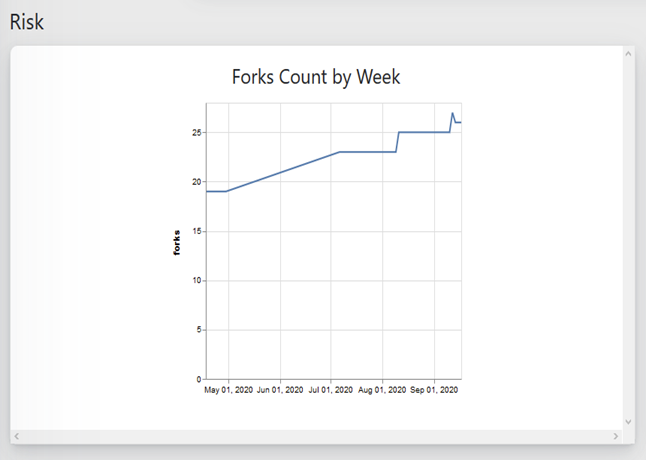
\includegraphics{images/technical-fork_augur-fork.png}

\textbf{GrimoireLab Implementation}\\
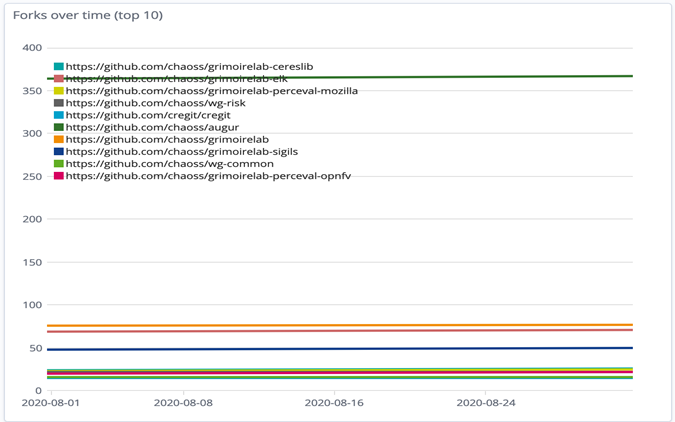
\includegraphics{images/technical-fork_grimoirelab-fork.png}

\hypertarget{tools-providing-the-metric}{%
\subparagraph{Tools Providing the
Metric}\label{tools-providing-the-metric}}

\begin{itemize}
\tightlist
\item
  Augur
\item
  GrimoireLab
\end{itemize}

\hypertarget{data-collection-strategies}{%
\subparagraph{Data Collection
Strategies}\label{data-collection-strategies}}

\textbf{Github API}\\
\url{https://developer.github.com/v3/repos/forks/\#list-forks}

\textbf{GitLab API}\\
\url{https://docs.gitlab.com/ee/api/projects.html\#list-forks-of-a-project}

\textbf{Bitbucket API}\\
\url{https://developer.atlassian.com/bitbucket/api/2/reference/resource/repositories/\%7Bworkspace\%7D/\%7Brepo_slug\%7D/forks}

\hypertarget{references}{%
\paragraph{References}\label{references}}

\url{https://help.github.com/en/enterprise/2.13/user/articles/fork-a-repo}
\url{https://opensource.com/article/17/12/fork-clone-difference}
 
\hypertarget{ux8d21ux732eux7c7bux578b}{%
\subsubsection{贡献类型}\label{ux8d21ux732eux7c7bux578b}}

问题:正在进行哪些类型的贡献?

\hypertarget{ux63cfux8ff0}{%
\paragraph{描述}\label{ux63cfux8ff0}}

多元化的贡献能够使开源项目健康发展。在很多项目中,有些社区成员并不编写代码,但他们同样做出了有价值的贡献,比如管理社区、区分错误、宣传项目、支持用户或以其他方式提供帮助。

\hypertarget{ux76eeux6807}{%
\paragraph{目标}\label{ux76eeux6807}}

多样的贡献类型表明项目是成熟全面的,包含足够的活动来支持项目的所有方面,并且提供多种贡献类型的晋升渠道,让拥有编码之外的不同专长的人员也能够发展到领导层。

\hypertarget{ux5b9eux73b0}{%
\paragraph{实现}\label{ux5b9eux73b0}}

如何对贡献进行定义、量化、跟踪和公布是一个具有挑战性的问题。
每个项目的答案可能都是独一无二的,以下建议仅作为抛砖引玉。作为一个通用指南,很难将不同的贡献类型相互比较,应单独考量。

\begin{itemize}
\tightlist
\item
  以下列表可以帮助确定贡献类型:

  \begin{itemize}
  \tightlist
  \item
    编写代码
  \item
    审查代码
  \item
    错误分类
  \item
    质量保证和测试
  \item
    安全相关活动
  \item
    本地化和翻译
  \item
    事件组织
  \item
    文档编写
  \item
    社区建设和管理
  \item
    教学和教程构建
  \item
    故障排除和支持
  \item
    创意作品和设计
  \item
    用户界面、用户体验和易用性
  \item
    社交媒体管理
  \item
    用户支持和问题解答
  \item
    撰写文章
  \item
    公共关系 - 技术媒体采访
  \item
    事件发言
  \item
    营销与活动宣传
  \item
    网站开发
  \item
    法律委员会
  \item
    财务管理
  \end{itemize}
\end{itemize}

\hypertarget{ux6570ux636eux6536ux96c6ux7b56ux7565}{%
\subparagraph{数据收集策略}\label{ux6570ux636eux6536ux96c6ux7b56ux7565}}

\begin{itemize}
\item
  **采访或调查:**让社区成员认可他人的贡献,找出过去没有考虑到的贡献类型。

  \begin{itemize}
  \tightlist
  \item
    您想表彰谁在项目中的贡献? 他们贡献了什么?
  \end{itemize}
\item
  **观察项目:**找出和认可项目不同部分的负责人。

  \begin{itemize}
  \tightlist
  \item
    在项目网站或代码仓库中列出了哪些负责人?
  \end{itemize}
\item
  **捕获非代码贡献:**通过问题跟踪器等专用系统跟踪贡献。

  \begin{itemize}
  \tightlist
  \item
    日志记录可以包含项目要了解的关于非代码贡献的定制化信息,用以识别工作量。
  \item
    通过沟通渠道活动的代理贡献。 例如,如果质量保证成员 (QA)
    拥有自己的邮件列表,就可以通过邮件列表活动来代理衡量围绕 QA
    贡献的活动。
  \end{itemize}
\item
  **收集跟踪数据:**通过协作工具日志数据衡量贡献。

  \begin{itemize}
  \tightlist
  \item
    例如,可以从源代码仓库计算代码贡献,可以从维基编辑历史记录计算维基贡献,可以从电子邮件归档计算电子邮件消息
  \end{itemize}
\item
  **自动分类:**训练人工智能 (AI) 机器人来检测贡献并对其分类。

  \begin{itemize}
  \tightlist
  \item
    AI
    机器人可以协助对贡献进行分类,例如,帮助请求与提供的支持,或功能请求与错误报告,尤其是以上均在同一个问题跟踪器中完成的情况。
  \end{itemize}
\end{itemize}

\emph{其他考量:}

\begin{itemize}
\tightlist
\item
  特别是对于自动报告,允许社区成员选择退出并不出现在贡献报告上。
\item
  承认对贡献类型的捕捉不完善,并明确说明收集了哪些类型的贡献。
\item
  随着项目发展,贡献类型的收集方法需要作出调整。
  例如,交换国际化库时,围绕本地化的项目活动可能会在变化前后产生不同的指标。
\item
  大规模挖掘贡献类型时,要考虑机器人的活动。
\end{itemize}

\hypertarget{ux53c2ux8003ux8d44ux6599}{%
\paragraph{参考资料}\label{ux53c2ux8003ux8d44ux6599}}

\begin{itemize}
\tightlist
\item
  \href{https://medium.com/@sunnydeveloper/revisiting-the-word-recognition-in-foss-and-the-dream-of-open-credentials-d15385d49447}{https://medium.com/@sunnydeveloper/revisiting-the-word-recognition-in-foss-and-the-dream-of-open-credentials-d15385d49447}
\item
  \href{https://24pullrequests.com/contributing}{https://24pullrequests.com/contributing}
\item
  \href{https://smartbear.com/blog/test-and-monitor/14-ways-to-contribute-to-open-source-without-being/}{https://smartbear.com/blog/test-and-monitor/14-ways-to-contribute-to-open-source-without-being/}
\item
  \href{https://wiki.openstack.org/wiki/AUCRecognition}{https://wiki.openstack.org/wiki/AUCRecognition}
\item
  \href{https://www.drupal.org/drupalorg/blog/a-guide-to-issue-credits-and-the-drupal.org-marketplace}{https://www.drupal.org/drupalorg/blog/a-guide-to-issue-credits-and-the-drupal.org-marketplace}
\end{itemize}
 
 

\subsection{Focus Area - When}
\textbf{Goal:} Understand when contributions from organizations and people are happening.
\begin{table}[ht!]
    \centering
    \begin{tabular}{|p{0.35\linewidth} | p{0.6\linewidth}|}
        \hline
        \hfil \textbf{Metric}  & \hfil \textbf{Question} \\
        \hline
		Activity Dates and Times & What are the dates and timestamps of when contributor activities occur? \\ 
		\hline
		Burstiness & How are short timeframes of intense activity, followed by a corresponding return to a typical pattern of activity, observed in a project? \\ 
		\hline
		Review Cycle Duration within a Change Request & What is the duration of a review cycle within a single change request? \\ 
		\hline
		Time to Close & How much time passes between creating and closing an operation such as an issue, change request, or support ticket? \\ 
		\hline
		Time to First Response & How much time passes between when an activity requiring attention is created and the first response? \\ 
		\hline
    \end{tabular}
\end{table}

\hypertarget{activity-dates-and-times}{%
\section{Activity Dates and Times}\label{activity-dates-and-times}}

Question: What are the dates and timestamps of when contributor
activities occur?

\hypertarget{description}{%
\subsection{Description}\label{description}}

Individuals engage in activities in open source projects at various
times of the day. This metric is aimed at determining the dates and
times of when individual activities were completed. The data can be used
to probabilistically estimate where on earth contributions come from in
cases where the time zone is not UTC.

\hypertarget{objectives}{%
\subsection{Objectives}\label{objectives}}

\begin{itemize}
\tightlist
\item
  Improve transparency for employers about when organizational employees
  are engaging with open source projects
\item
  Improve transparency for open source project and community managers as
  to when activity is occurring
\end{itemize}

\hypertarget{implementation}{%
\subsection{Implementation}\label{implementation}}

\hypertarget{filters}{%
\subsubsection{Filters}\label{filters}}

\begin{itemize}
\tightlist
\item
  Individual by Organization
\item
  Aggregation of time by UTC time

  \begin{itemize}
  \tightlist
  \item
    Can show what times across the globe contributions are made; when
    the project is most active.
  \end{itemize}
\item
  Aggregation of time by local time

  \begin{itemize}
  \tightlist
  \item
    Can show what times of day in their local times they contribute.
    Conclusions about the If contributions are more during working
    hours, or if contributions are more during evening hours.
  \end{itemize}
\item
  Repository ID
\item
  Segment of a community, (e.g., GrimoireLab has more EU time zones
  activity and Augur more US time zones activity)
\end{itemize}

\hypertarget{visualizations}{%
\subsubsection{Visualizations}\label{visualizations}}

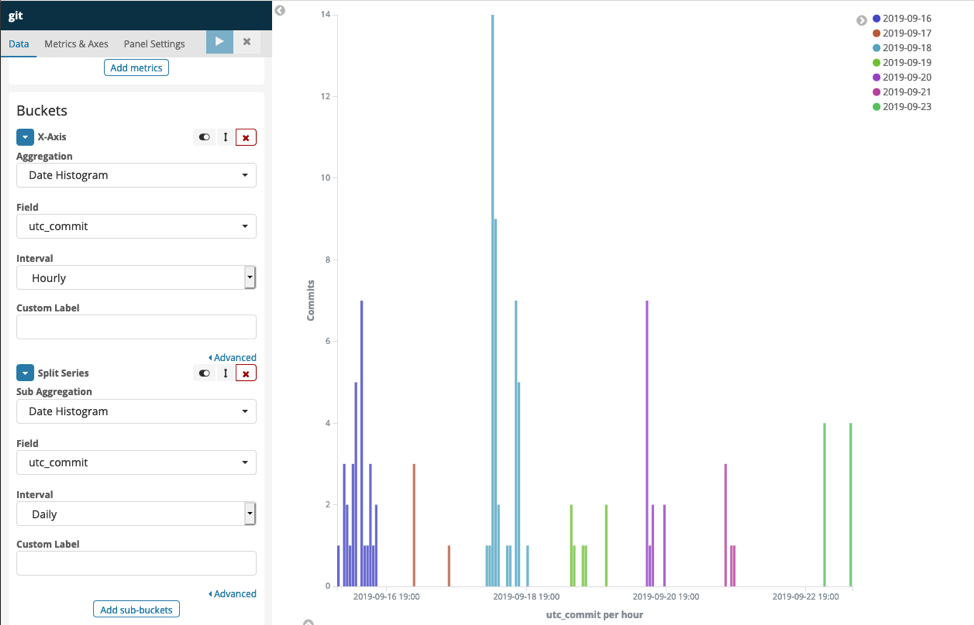
\includegraphics{images/activity-dates-and-times_1.png}
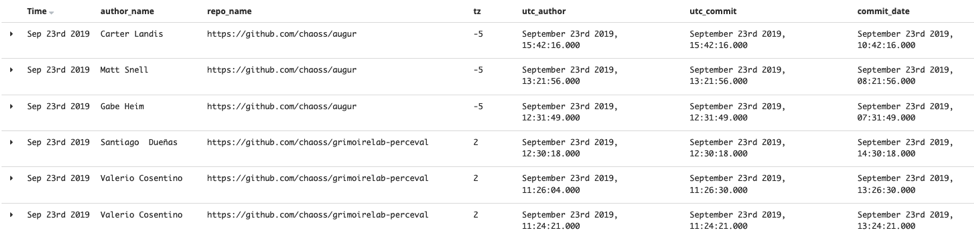
\includegraphics{images/activity-dates-and-times_2.png}
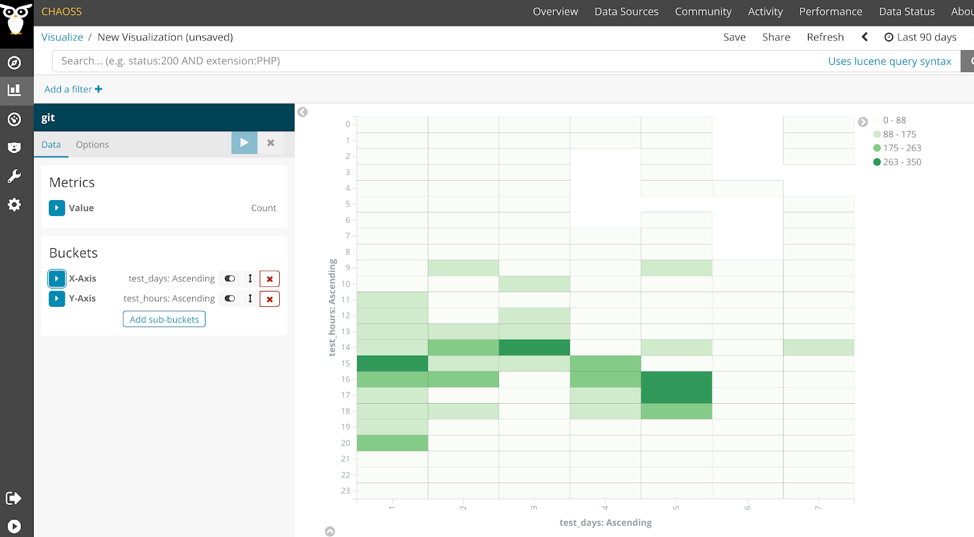
\includegraphics{images/activity-dates-and-times_3.png}
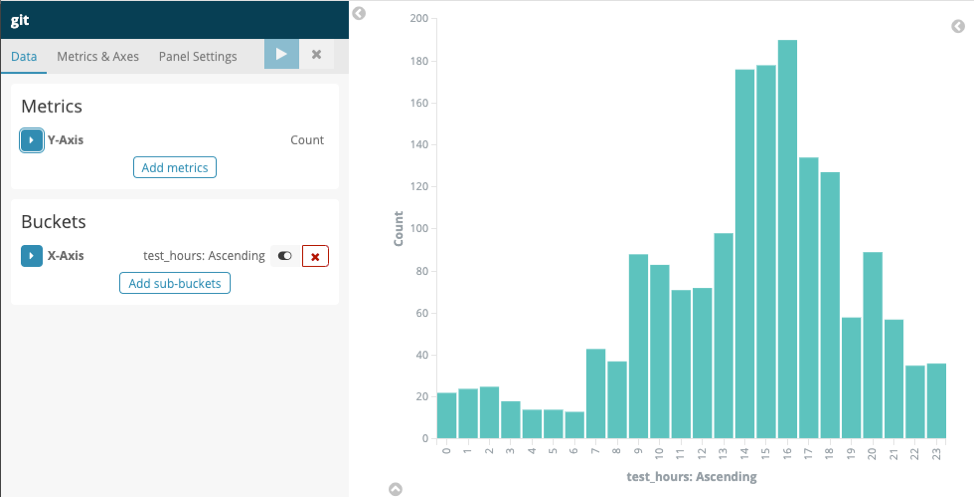
\includegraphics{images/activity-dates-and-times_4.png}

\hypertarget{tools-providing-metric}{%
\subsubsection{Tools Providing Metric}\label{tools-providing-metric}}

\href{https://chaoss.github.io/grimoirelab/}{GrimoireLab}

\href{https://docs.augur.net/\#dates-timestamps}{Augur Date/Timestamps}

\hypertarget{references}{%
\subsection{References}\label{references}}

\href{https://en.wikipedia.org/wiki/Coordinated_Universal_Time}{Coordinated
Universal Time}
 
\hypertarget{burstiness}{%
\section{Burstiness}\label{burstiness}}

Question: How are short timeframes of intense activity, followed by a
corresponding return to a typical pattern of activity, observed in a
project?

\hypertarget{description}{%
\subsection{Description}\label{description}}

There are a number of reasons that may prompt a sudden increase or
decrease in the amount of activity within a repository. These increases
and decreases appear both as a sudden change in activity against the
average amount of activity. Burstiness is a way of understanding the
cycle of activity in existing metrics, like issues, merge requests,
mailing lists, commits, or comments. Examples of root causes for bursts
in activity include:

\begin{itemize}
\tightlist
\item
  Release cycles
\item
  Global pandemics
\item
  Hackathon activities
\item
  Mentorship programs
\item
  Conferences, meetups, and other events where tools are presented
\item
  Conventional and social media announcements and mentions
\item
  Critical bugs as raising awareness and getting people's attention
\item
  Community design meetings or brainstorming meetings to address a
  particular issue
\item
  Community members show up from another community that is relying on
  your project (e.g., dependencies)
\end{itemize}

\hypertarget{objectives}{%
\subsection{Objectives}\label{objectives}}

\begin{itemize}
\tightlist
\item
  To identify impacts of root causes of a burst in activity
\item
  To provide awareness when project activity unknowingly goes up
\item
  To help capture the meaningfulness of increases or decreases in
  project activity
\item
  To help the community and maintainers prepare for future bursts that
  follow a pattern
\item
  To help measure the impact of influential external activities
\item
  To differentiate skewed activity versus normal activity
\end{itemize}

\hypertarget{implementation}{%
\subsection{Implementation}\label{implementation}}

\hypertarget{filters}{%
\subsubsection{Filters}\label{filters}}

\begin{itemize}
\tightlist
\item
  Stars
\item
  Forks
\item
  Issues or bug reports
\item
  Labels
\item
  Downloads
\item
  Release Tags
\item
  Change Requests
\item
  Mail List Traffic
\item
  Documentation additions or revisions
\item
  New Repositories
\item
  Feature Requests
\item
  Messaging Conversations
\item
  Conventional and Social Media Activity
\item
  Conference Attendance and Submissions
\end{itemize}

\hypertarget{visualizations}{%
\subsubsection{Visualizations}\label{visualizations}}

Augur:

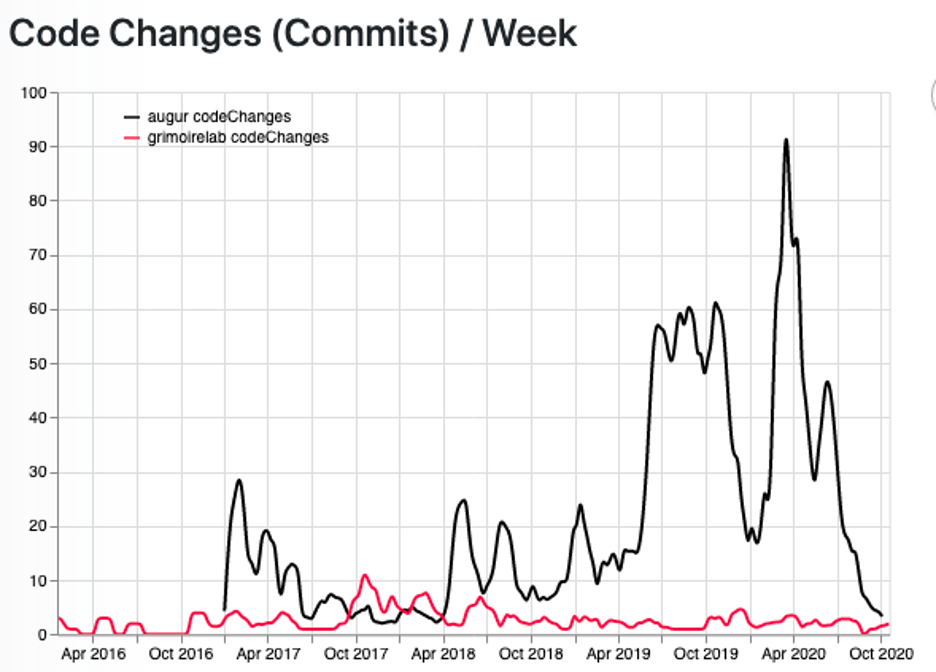
\includegraphics{images/burstiness_augur.png}

GrimoireLab:

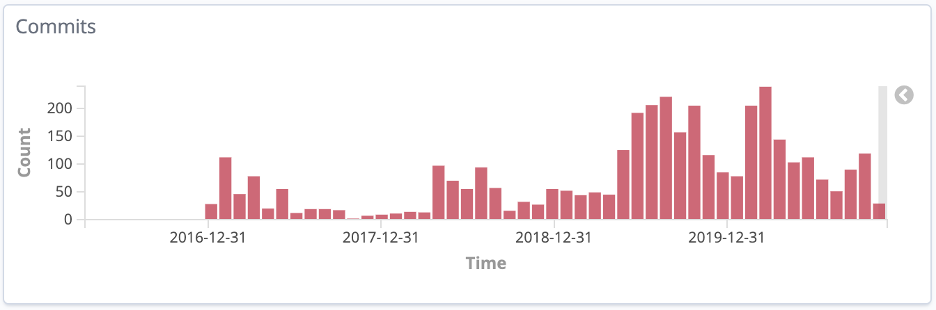
\includegraphics{images/burstiness_gl.png}

\hypertarget{tools-providing-the-metric}{%
\subsubsection{Tools Providing the
Metric}\label{tools-providing-the-metric}}

\begin{itemize}
\tightlist
\item
  Grimoire Lab
\item
  Augur
\end{itemize}

\hypertarget{data-collection-strategies}{%
\subsubsection{Data Collection
Strategies}\label{data-collection-strategies}}

\begin{itemize}
\item
  Quantitative

  \begin{itemize}
  \tightlist
  \item
    Time box activities identifying deviations away from some norm
  \item
    Outliers for certain thresholds, using statistics like Bollinger
    Bands to measure stability or volatility:
    \url{https://en.wikipedia.org/wiki/Bollinger_Bands}
  \end{itemize}
\item
  Qualitative Interview Questions

  \begin{itemize}
  \tightlist
  \item
    Why do you contribute more during a period of time?
  \item
    What do you believe to be the root cause for particular bursts?
  \item
    What impact do different events (e.g., hackathons, mentorship
    program, or conferences) have on project activity?
  \end{itemize}
\end{itemize}

\hypertarget{references}{%
\subsection{References}\label{references}}

This metric was inspired by the work of Goh and Barabasi (2008):
\url{https://arxiv.org/pdf/physics/0610233.pdf}
 
\hypertarget{review-cycle-duration-within-a-change-request}{%
\subsubsection{Review Cycle Duration within a Change
Request}\label{review-cycle-duration-within-a-change-request}}

Question: What is the duration of a review cycle within a single change
request?

\hypertarget{description}{%
\paragraph{Description}\label{description}}

A change request is based on one or more review cycles. Within a review
cycle, one or more reviewers can provide feedback on a proposed
contribution. The duration of a review cycle, or the time between each
new iteration of the contribution, is the basis of this metric.

\hypertarget{objectives}{%
\paragraph{Objectives}\label{objectives}}

This metric provides maintainers with insight on: Code review process
decay, as there are more iterations and review cycle durations increase.
Process bottlenecks resulting in long code review iterations. Abandoned
or semi-abandoned processes in the review cycles, where either the
maintainer or the submitter is slow in responding. Characteristics of
reviews that have different cyclic pattern lengths.

\hypertarget{implementation}{%
\paragraph{Implementation}\label{implementation}}

Review Cycle Duration is measured as the time length of one review cycle
within a single change request. The duration can be calculated between:
The moment when each review cycle begins, defined as the point in time
when a change request is submitted or updated. The moment when each
review cycle ends, either because the change request was updated and
needs a new review or because it was accepted or rejected.

\hypertarget{filter}{%
\subparagraph{Filter}\label{filter}}

Average or Median Duration, optionally filtered or grouped by: Number of
people involved in review Number of comments in review Edits made to a
change request Project or program Organization making the change request
Time the change request was submitted Developers who contributed to a
change request Change request Number of review cycle on a change request
(e.g., filter by first, second, \ldots{} round)

\hypertarget{visualizations}{%
\subparagraph{Visualizations}\label{visualizations}}

\hypertarget{tools-providing-the-metric}{%
\subparagraph{Tools Providing the
Metric}\label{tools-providing-the-metric}}

\hypertarget{references}{%
\paragraph{References}\label{references}}

Example of data that could be used to develop the metric:
\url{https://gerrit.wikimedia.org/r/c/mediawiki/core/+/194071}
 
\hypertarget{ux5173ux95edux65f6ux957f}{%
\subsubsection{关闭时长}\label{ux5173ux95edux65f6ux957f}}

问题:创建和关闭操作(如议题、更改请求或需要支持的问题单)之间需要多少时间?

\hypertarget{ux63cfux8ff0}{%
\paragraph{描述}\label{ux63cfux8ff0}}

关闭时长是指从创建到关闭操作(如议题、更改请求或需要支持的问题单)的总时长。
操作需要具有打开和关闭的状态,比如代码审查进程、问答论坛、问题跟踪系统中经常出现的情况。

相关指标:\href{https://chaoss.community/metric-issue-resolution-duration/}{问题解决时长}

\hypertarget{ux76eeux6807}{%
\paragraph{目标}\label{ux76eeux6807}}

\begin{enumerate}
\def\labelenumi{\arabic{enumi}.}
\tightlist
\item
  确定社区的响应程度,帮助增加包容性,吸引新贡献者并保留现有贡献者。
\item
  找出导致快速或缓慢关闭的操作特征(如寻找最佳实践、改进领域、评估效率)。
\item
  识别对不同社区成员及时响应的偏差。
\item
  检测社区活动的变化(例如,显示潜在的维护者倦怠、贡献多元化的减少)
\item
  了解关闭议题或更改请求的时间与合并成功或失败的关系
\end{enumerate}

\hypertarget{ux5b9eux73b0}{%
\paragraph{实现}\label{ux5b9eux73b0}}

\hypertarget{ux7b5bux9009ux6761ux4ef6}{%
\subparagraph{筛选条件}\label{ux7b5bux9009ux6761ux4ef6}}

\begin{itemize}
\tightlist
\item
  操作的创建者(例如,新贡献者相对于维护者)
\item
  最初关闭,最后关闭
\item
  标签(例如错误与新功能)
\item
  更改请求合并状态(例如,合并时间或没有合并的关闭时间)
\end{itemize}

\hypertarget{ux53efux89c6ux5316ux6548ux679c}{%
\subparagraph{可视化效果}\label{ux53efux89c6ux5316ux6548ux679c}}

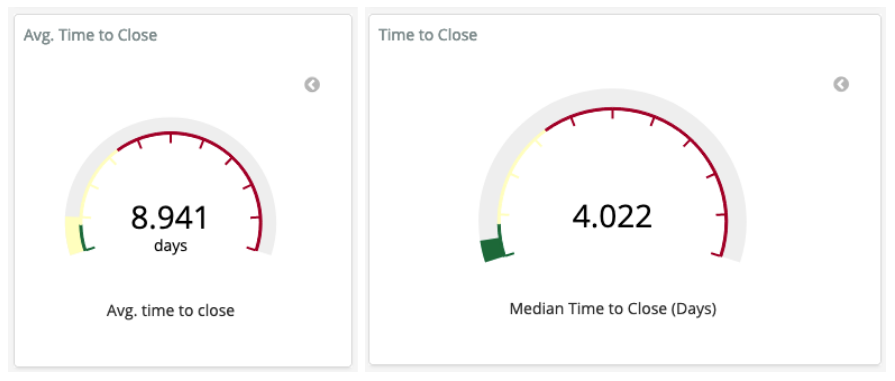
\includegraphics{images/time-to-close_1.png}

\hypertarget{ux63d0ux4f9bux6307ux6807ux7684ux5de5ux5177}{%
\subparagraph{提供指标的工具}\label{ux63d0ux4f9bux6307ux6807ux7684ux5de5ux5177}}

Augur 实现:

\begin{itemize}
\tightlist
\item
  \href{http://augur.osshealth.io/api_docs/\#api-Evolution-Closed_Issue_Resolution_Duration(Repo)}{问题解决时长}
\item
  \href{http://augur.osshealth.io/api_docs/\#api-Evolution-issue-duration-repo}{问题持续时间}
\item
  \href{http://augur.osshealth.io/api_docs/\#api-Evolution-Issue_Response_Time(Repo)}{问题响应时间}
\end{itemize}

GrimoireLab 实现:

\begin{itemize}
\tightlist
\item
  \href{https://chaoss.github.io/grimoirelab-sigils/panels/github-pullrequests-efficiency/}{拉取请求效率}
\item
  \href{https://chaoss.github.io/grimoirelab-sigils/panels/github-issues-efficiency/}{问题效率}
\item
  \href{https://chaoss.github.io/grimoirelab-sigils/panels/efficiency-timing-overview/}{Efficiency:TimingOverview}
\end{itemize}

\hypertarget{ux6570ux636eux6536ux96c6ux7b56ux7565}{%
\subparagraph{数据收集策略}\label{ux6570ux636eux6536ux96c6ux7b56ux7565}}

关闭时长指标可根据项目活动和目标的具体情况而定。
例如,错误报告的关闭时长可能提供与新功能请求的关闭时长不同的信息。
数据收集策略应针对不同的项目目标。 可能影响这些进程的其他变量是:

\begin{itemize}
\tightlist
\item
  问题跟踪系统:如错误报告、蓝图 (OpenStack 专有命名)、用户故事(user
  story)、功能请求、epic等可能会影响事件关闭时长的议题类型。
  优先级或严重性等其他变量可能有助于推进这一事件的关闭速度。
\item
  变更请求流程:这取决于变更请求的平台架构,如 Gerrit、GitHub
  或邮件列表(如 Linux 内核中),并可能根据进程的复杂程度而有所不同。
  例如,新人和经验丰富的高级开发者将以不同的方式开展进程,所需时间或多或少。
\item
  问答论坛:这取决于回答的质量和提问者的意见。
  有效答案会被标记,提问者成功找到自己问题的正确答案后,进程随即关闭。
\end{itemize}

\hypertarget{ux53c2ux8003ux8d44ux6599}{%
\paragraph{参考资料}\label{ux53c2ux8003ux8d44ux6599}}

\begin{itemize}
\tightlist
\item
  ``Practice P.12: Respond to all submissions'',出自``Appendix to:
  Managing Episodic Volunteers in Free/Libre/Open Source Software
  Communities'',Ann Barcomb、Klaas-Jan Stol、Brian Fitzgerald 和 Dirk
  Riehle:\href{https://opus4.kobv.de/opus4-fau/frontdoor/index/index/docId/13519}{https://opus4.kobv.de/opus4-fau/frontdoor/index/index/docId/13519}
\end{itemize}
 
\hypertarget{time-to-first-response}{%
\subsubsection{Time to First Response}\label{time-to-first-response}}

Question: How much time passes between when an activity requiring
attention is created and the first response?

\hypertarget{description}{%
\paragraph{Description}\label{description}}

The first response to an activity can sometimes be the most important
response. The first response shows that a community is active and
engages in conversations. A long time to respond to an activity can be a
sign that a community is not responsive. A short time to respond to an
activity can help to engage more members into further discussions and
within the community.

\hypertarget{objectives}{%
\paragraph{Objectives}\label{objectives}}

Identify cadence of first response across a variety of activities,
including PRs, Issues, emails, IRC posts, etc. Time to first response is
an important consideration for new and long-time contributors to a
project along with overall project health.

\hypertarget{implementation}{%
\paragraph{Implementation}\label{implementation}}

Time to first response of an activity = time first response was posted
to the activity - time the activity was created.

\hypertarget{filters}{%
\subparagraph{Filters}\label{filters}}

\begin{itemize}
\tightlist
\item
  Role of responder, e.g., only count maintainer responses
\item
  Automated responses, e.g., only count replies from real people by
  filtering bots and other automated replies
\item
  Type of Activity, e.g., issues (see metric
  \href{https://github.com/chaoss/wg-evolution/blob/master/metrics/Issue_Response_Time.md}{Issue
  Response Time}), emails, chat, change requests
\end{itemize}

\hypertarget{visualizations}{%
\subparagraph{Visualizations}\label{visualizations}}

<<<<<<< HEAD
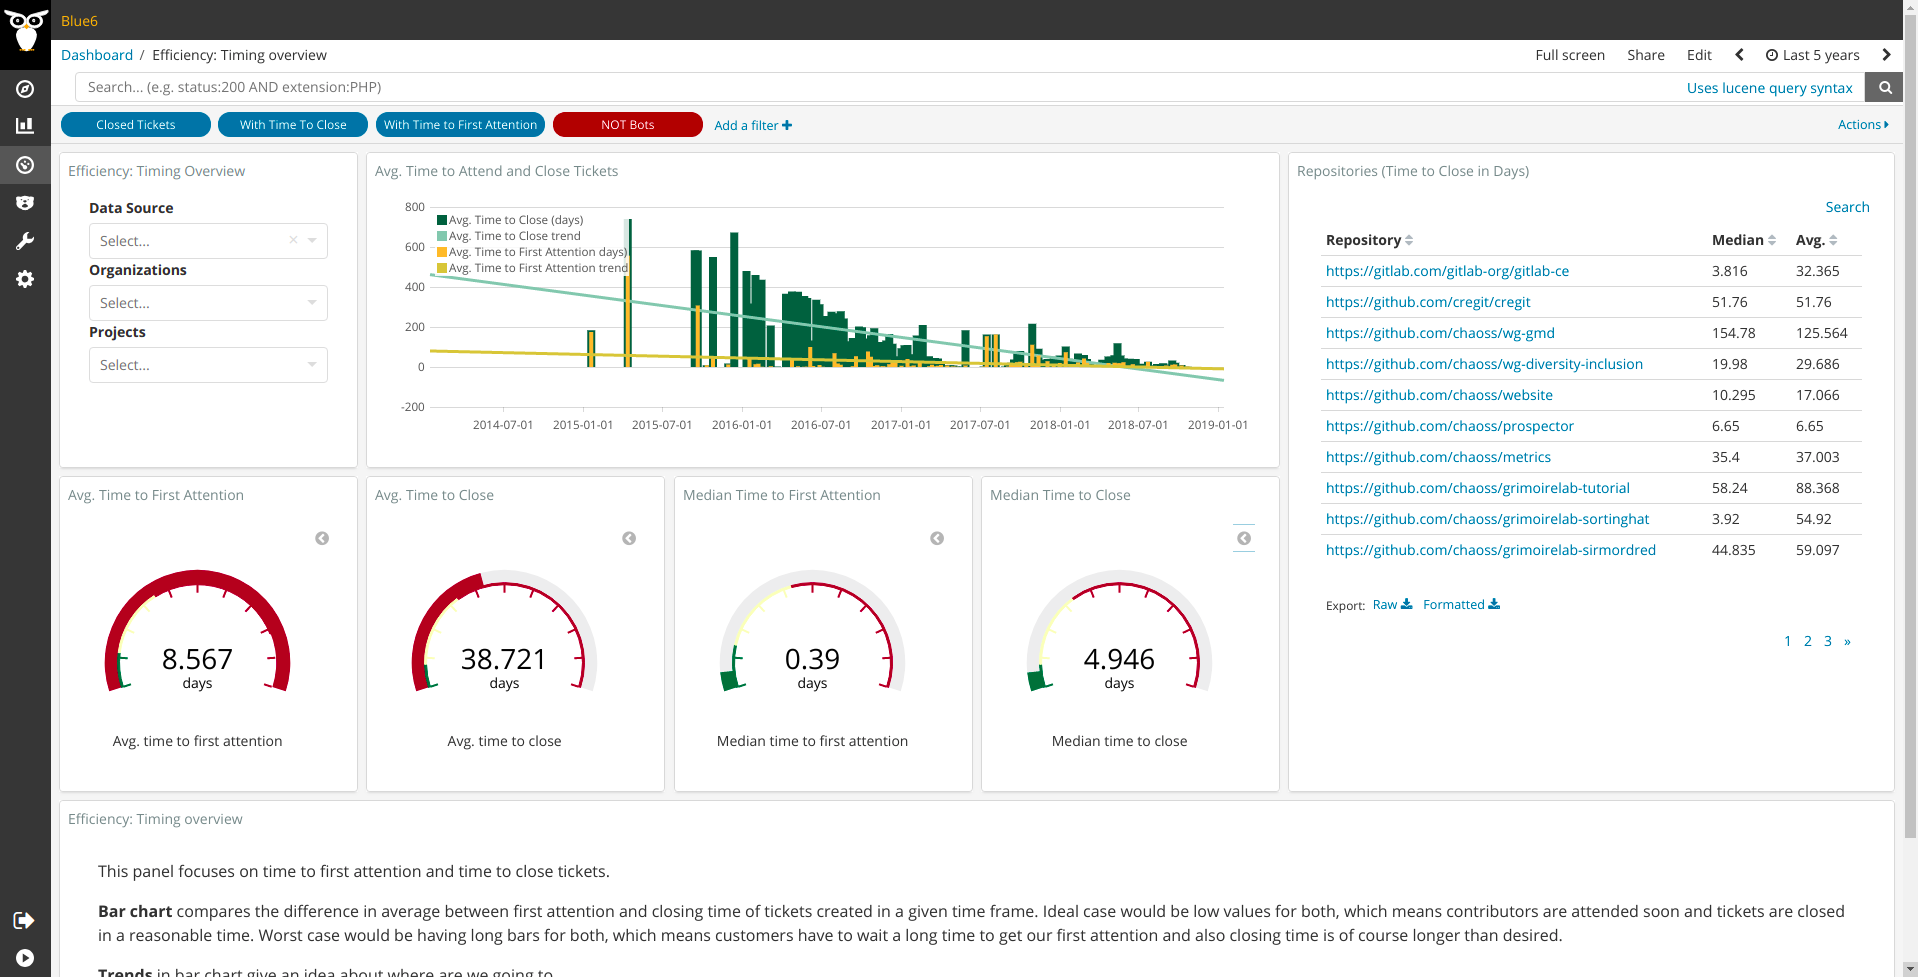
\includegraphics{images/time-to-first-response_efficiency-timing-overview.png}

\begin{center}\rule{0.5\linewidth}{0.5pt}\end{center}

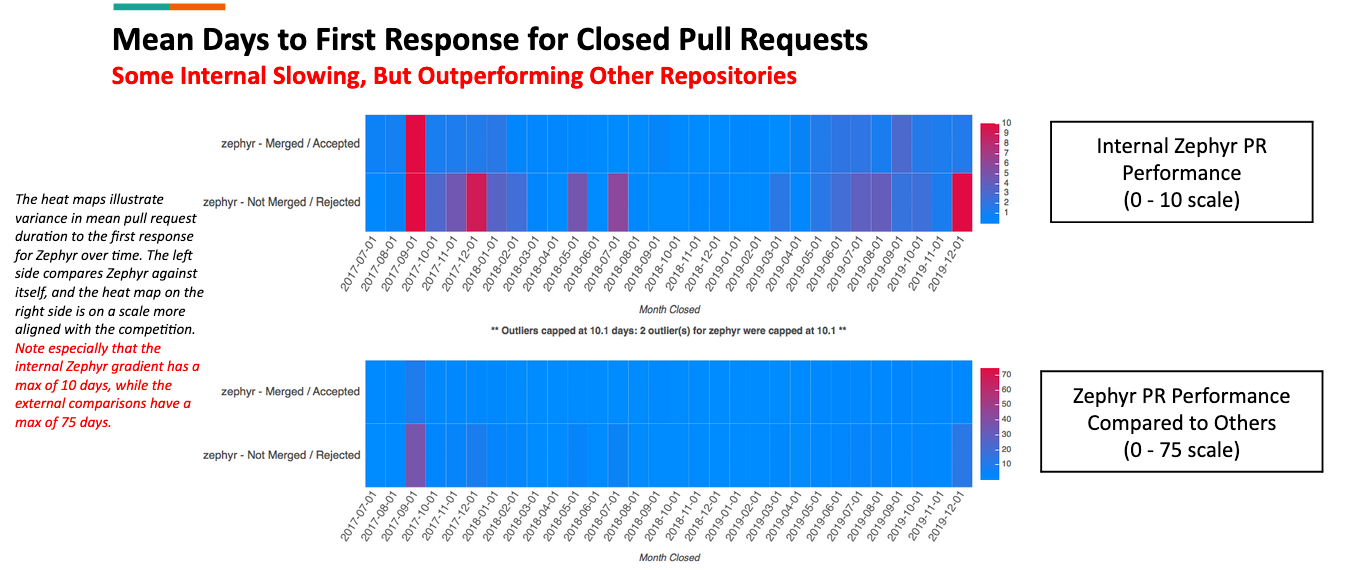
\includegraphics{images/time-to-first-response_augur-ttc-1.png}

\begin{center}\rule{0.5\linewidth}{0.5pt}\end{center}
=======
\hypertarget{grimoirelab-panel-efficiency-timing-overview}{%
\subsection{\texorpdfstring{\protect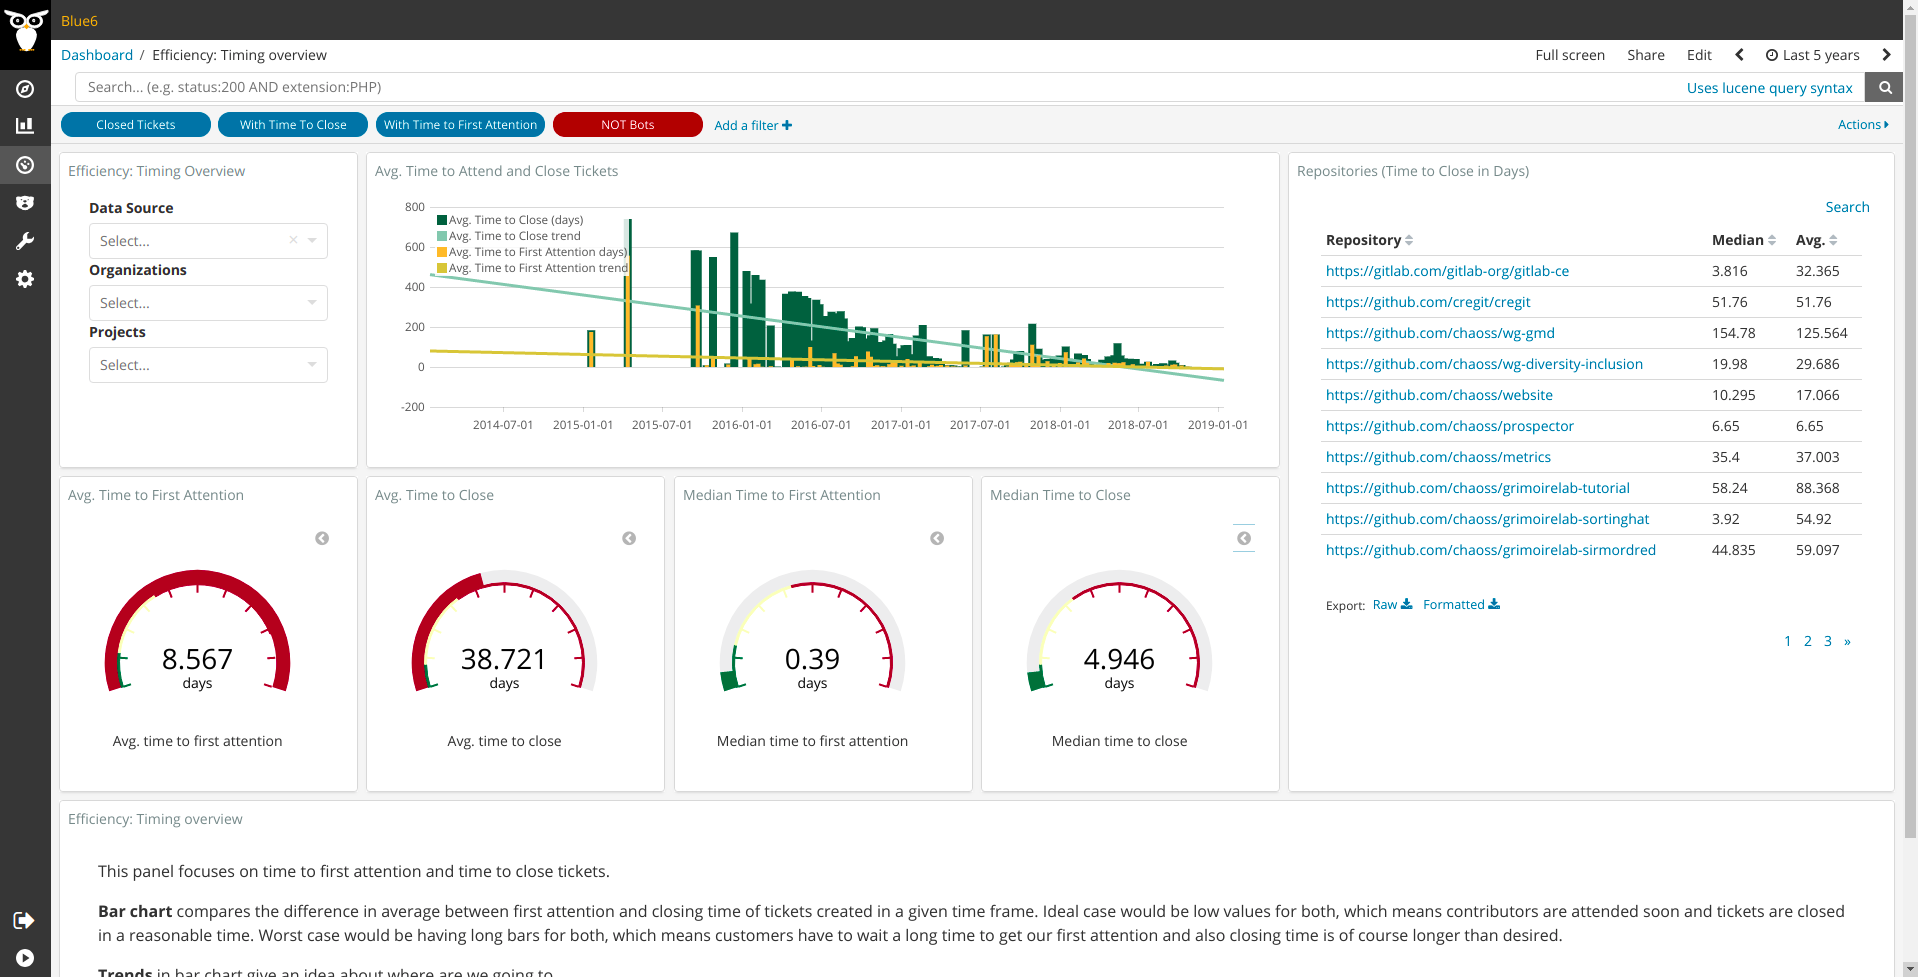
\includegraphics{images/time-to-first-response_efficiency-timing-overview.png}}{GrimoireLab Panel: Efficiency Timing Overview}}\label{grimoirelab-panel-efficiency-timing-overview}}

\hypertarget{augur-visualization-time-to-first-response-heat-map-}{%
\subsection{\texorpdfstring{\protect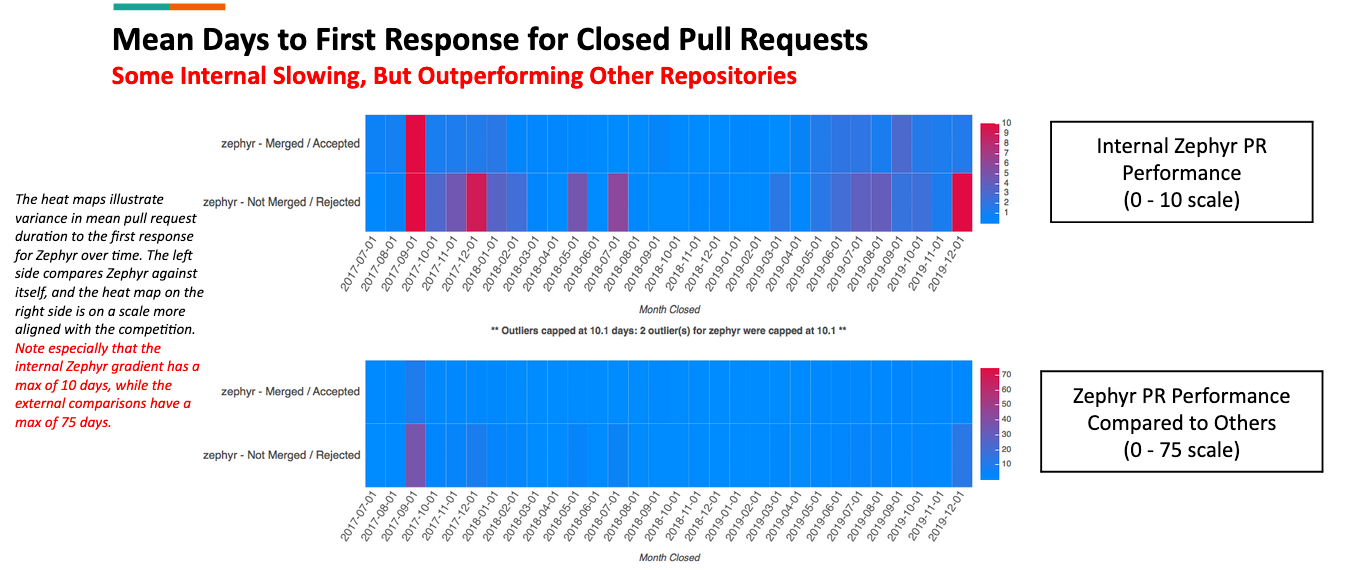
\includegraphics{images/time-to-first-response_augur-ttc-1.png}}{Augur Visualization: Time to First Response Heat Map }}\label{augur-visualization-time-to-first-response-heat-map-}}
>>>>>>> main

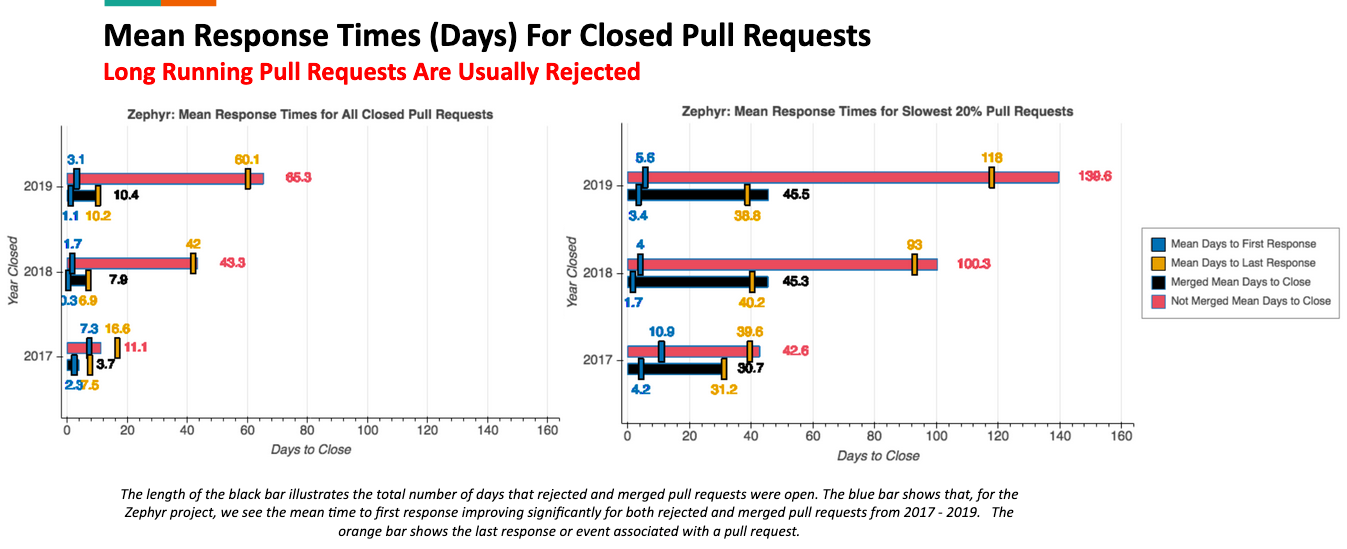
\includegraphics{images/time-to-first-response_augur-ttc-2.png}

\hypertarget{tools-providing-the-metric}{%
\subparagraph{Tools Providing the
Metric}\label{tools-providing-the-metric}}

\begin{itemize}
\tightlist
\item
  GrimoireLab Panel:
  \href{https://chaoss.github.io/grimoirelab-sigils/panels/efficiency-timing-overview/}{Efficiency
  Timing Overview}
\item
  \href{https://katacontainers.biterg.io/app/kibana\#/dashboard/cbbdd920-288c-11e9-b662-975152e57997}{Kata
  Containers dashboard efficiency panel}
\end{itemize}

\hypertarget{references}{%
\paragraph{References}\label{references}}
 
 

\subsection{Focus Area - who}
\textbf{Goal:} Understand organizational and personal engagement with open source projects
\begin{table}[ht!]
    \centering
    \begin{tabular}{|p{0.35\linewidth} | p{0.6\linewidth}|}
        \hline
        \hfil \textbf{Metric}  & \hfil \textbf{Question} \\
        \hline
		Contributor Location & What is the location of contributors? \\ 
		\hline
		Contributors & Who are the contributors to a project? \\ 
		\hline
		Organizational Diversity & What is the organizational diversity of contributions? \\ 
		\hline
    \end{tabular}
\end{table}
 
 


    \section{Value WG}
    \begin{table}[ht!]
        \centering
        \begin{tabular}{|p{0.35\linewidth} | p{0.6\linewidth}|}
            \hline
            \hfil \textbf{关注领域}  & \hfil \textbf{目标} \\
            \hline
        		公共价值 & 确定项目(包括下游项目)是否对社区用户或者贡献者有价值。 \\ 
		\hline
		Placeholder & Placeholder \\ 
		\hline
		人力投资 & 从组织的角度看项目是否具有经济价值。 \\ 
		\hline
    \end{tabular}
    \end{table}
        
\clearpage

    \subsection{关注领域 - 公共价值}
    \textbf{目标:} 确定项目(包括下游项目)是否对社区用户或者贡献者有价值。
    \begin{table}[ht!]
        \centering
        \begin{tabular}{|p{0.35\linewidth} | p{0.6\linewidth}|}
            \hline
            \hfil \textbf{度量指标}  & \hfil \textbf{问题} \\
            \hline
        		项目发展速度 & 如何衡量组织的发展速度? \\ 
		\hline
    \end{tabular}
    \end{table}
        
\hypertarget{project-velocity}{%
\subsubsection{Project Velocity}\label{project-velocity}}

Question: What is the development speed for an organization?

\hypertarget{description}{%
\paragraph{Description}\label{description}}

Project velocity is the number of issues, the number of pull requests,
volume of commits, and number of contributors as an indicator of
'innovation'.

\hypertarget{objectives}{%
\paragraph{Objectives}\label{objectives}}

Gives an Open Source Program Office (OSPO) manager a way to compare the
project velocity across a portfolio of projects.

The OSPO manager can use the Project Velocity metric to:

\begin{itemize}
\tightlist
\item
  Report project velocity of open source projects vs in-house projects
\item
  Compare project velocity across a portfolio of projects
\item
  Identify which projects grow beyond internal contributors (when
  filtering internal vs. external contributors)
\item
  Identify promising areas in which to get involved
\item
  Highlight areas likely to be the successful platforms over the next
  several years
\end{itemize}

\href{https://www.cncf.io/blog/2017/06/05/30-highest-velocity-open-source-projects}{See
Example}

\hypertarget{implementation}{%
\paragraph{Implementation}\label{implementation}}

Base metrics include:

\begin{itemize}
\tightlist
\item
  \href{https://github.com/chaoss/wg-evolution/blob/master/metrics/Issues_Closed.md}{issues
  closed}
\item
  \href{https://github.com/chaoss/wg-evolution/blob/master/metrics/Reviews.md}{number
  of reviews}
\item
  \href{https://github.com/chaoss/wg-evolution/blob/master/metrics/Code_Changes.md}{\#
  of code changes}
\item
  \href{https://github.com/chaoss/wg-risk/blob/master/metrics/Committers.md}{\#
  of committers}
\end{itemize}

\hypertarget{filters}{%
\subparagraph{Filters}\label{filters}}

\begin{itemize}
\tightlist
\item
  Internal vs external contributors
\item
  Project sources (e.g., internal repositories, open-source
  repositories, and competitor open-source repositories)
\item
  Time
\end{itemize}

\hypertarget{visualizations}{%
\subparagraph{Visualizations}\label{visualizations}}

\begin{itemize}
\tightlist
\item
  X-Axis: Logarithmic scale for Code Changes
\item
  Y-Axis: Logarithmic scale of Sum of Number of Issues and Number of
  Reviews
\item
  Dot-size: Committers
\item
  Dots are projects
\end{itemize}

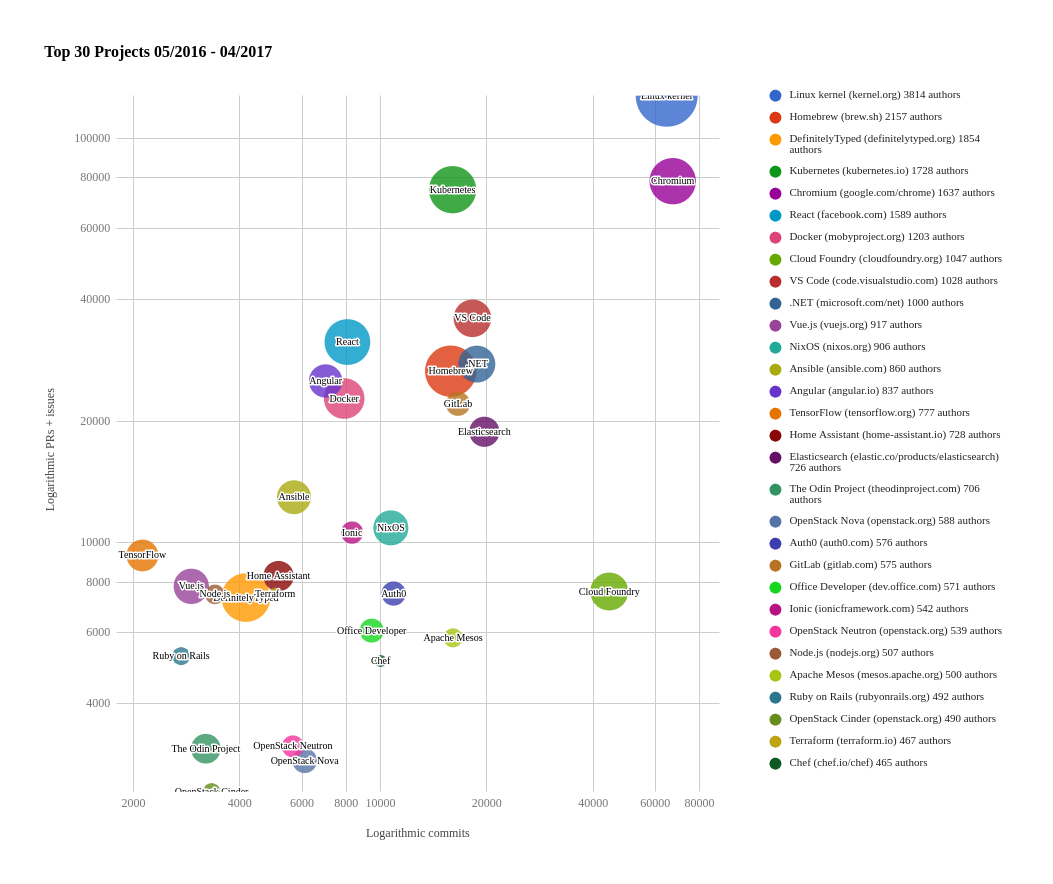
\includegraphics{images/project-velocity_visualization.png}

\href{https://www.cncf.io/blog/2017/06/05/30-highest-velocity-open-source-projects/}{From
CNCF}

\hypertarget{tools-providing-the-metric}{%
\subparagraph{Tools providing the
Metric}\label{tools-providing-the-metric}}

\begin{itemize}
\tightlist
\item
  CNCF -
  \href{https://github.com/cncf/velocity}{https://github.com/cncf/velocity}
\end{itemize}

\hypertarget{references}{%
\paragraph{References}\label{references}}

\begin{itemize}
\tightlist
\item
  \href{https://www.threefivetwo.com/blog/can-open-source-innovation-work-in-the-enterprise}{Can
  Open Source Innovation work in the Enterprise?}
\item
  \href{https://www.nearform.com/blog/want-a-high-performing-culture-make-way-for-open-innovation}{Open
  Innovation for a High Performance Culture}
\item
  \href{https://www.cio.com/article/3213146/open-source-is-powering-the-digital-enterprise.html}{Open
  Source for the Digital Enterprise}
\item
  \href{https://www.cncf.io/blog/2017/06/05/30-highest-velocity-open-source-projects}{Highest
  Velocity Open Source Projects}
\end{itemize}
 
 

\subsection{Focus Area - Individual-Value}
\textbf{Goal:} Identify if a project is valuable to me as an individual user or contributor.
\begin{table}[ht!]
    \centering
    \begin{tabular}{|p{0.35\linewidth} | p{0.6\linewidth}|}
        \hline
        \hfil \textbf{Metric}  & \hfil \textbf{Question} \\
        \hline
		Job Opportunities & How many job postings request skills with technologies from a project? \\ 
		\hline
		Organizational Project Skill Demand & How many organizations are using this project and could hire me if I become proficient? \\ 
		\hline
    \end{tabular}
\end{table}

\hypertarget{job-opportunities}{%
\section{Job Opportunities}\label{job-opportunities}}

Question: How many job postings request skills with technologies from a
project?

\hypertarget{description}{%
\subsection{Description}\label{description}}

A common way for open source contributors to earn a living wage is to be
employed by a company or be a self-employed or freelance developer.
Skills in a specific project may improve a job applicant's prospects of
getting a job. The most obvious indicator for demand related to a skill
learned in a specific open source project is when that project or its
technology is included in job postings.

\hypertarget{objectives}{%
\subsection{Objectives}\label{objectives}}

The metric gives contributors a sense of how much skills learned in a
specific open source project are valued by companies.

\hypertarget{implementation}{%
\subsection{Implementation}\label{implementation}}

To obtain this metric on a job search platform (e.g., LinkedIn, Indeed,
or Dice), go to the job search and type in the name of the open source
project. The number of returned job postings is the metric. Periodically
collecting the metric through an API of a job search platform and
storing the results allows to see trends.

\hypertarget{filters}{%
\subsubsection{Filters}\label{filters}}

\begin{itemize}
\tightlist
\item
  Age of job posting; postings get stale and may not be removed when
  filled
\end{itemize}

\hypertarget{visualizations}{%
\subsubsection{Visualizations}\label{visualizations}}

The metric can be extended by looking at:

\begin{itemize}
\tightlist
\item
  Salary ranges for jobs returned
\item
  Level of seniority for jobs returned
\item
  Availability of jobs like on-site or off-site
\item
  Location of job
\item
  Geography
\end{itemize}

\hypertarget{references}{%
\subsection{References}\label{references}}

\begin{itemize}
\tightlist
\item
  LinkedIn Job Search API:
  \url{https://developer.linkedin.com/docs/v1/jobs/job-search-api\#}
\item
  Indeed Job Search API:
  \url{https://opensource.indeedeng.io/api-documentation/docs/job-search/}
\item
  Dice.com Job Search API:
  \url{http://www.dice.com/external/content/documentation/api.html}
\item
  Monster Job Search API: \url{https://partner.monster.com/job-search}
\item
  Ziprecruiter API (Requires Partnership):
  \url{https://www.ziprecruiter.com/zipsearch}
\end{itemize}

\emph{Note:} This metric is limited to individual projects but
engagement in open source can be beneficial for other reasons. This
metric could be tweaked to look beyond a single project and instead use
related skills such as programming languages, processes, open source
experience, or frameworks as search parameters for jobs.
 
\hypertarget{organizational-project-skill-demand}{%
\section{Organizational Project Skill
Demand}\label{organizational-project-skill-demand}}

Question: How many organizations are using this project and could hire
me if I become proficient?

\hypertarget{description}{%
\subsection{Description}\label{description}}

Organizations engage with open source projects through use and
dependencies. This metric is aimed at determining downstream demand of
skills related to an open source project. This metric looks at
organizations that deploy a project as part of an IT infrastructure,
other open source projects with declared dependencies, and references to
the project through social media, conference mentions, blog posts, and
similar activities.

\hypertarget{objectives}{%
\subsection{Objectives}\label{objectives}}

As a developer, I'd like to invest my skills and time in a project that
has a likelihood of getting me a decent paying job in the future. People
can use the Downstream Organizational Impact of a Project Software
metric to discover which projects are used by organizations, and they
may, therefore, be able to pursue job opportunities with, possibly
requiring IT support services.

\hypertarget{implementation}{%
\subsection{Implementation}\label{implementation}}

Base metrics include:

\begin{itemize}
\tightlist
\item
  Number of organizations that created issues for a project
\item
  Number of organizations that created pull requests for a project
\item
  Number of organizations that blog or tweet about a project
\item
  Number of organizations that mention a project in open hiring requests
\item
  Number of organizations that are represented at meetups about this
  project
\item
  Number of other projects that are dependent on a project
\item
  Number of books about a project
\item
  Google search trends for a project
\end{itemize}

\hypertarget{visualizations}{%
\subsubsection{Visualizations}\label{visualizations}}

The following visualization demonstrates the number of downstream
projects dependendent on the project in question. While this
visualization does not capture the entirety of the Downstream
Organizational Impact of a Project Software metric, it provides a visual
for a portion.

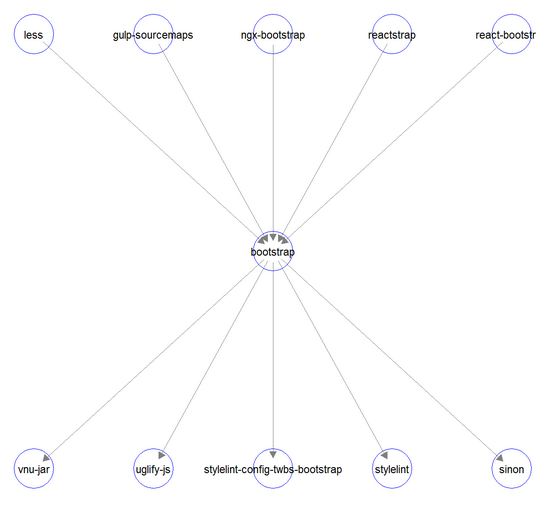
\includegraphics{images/organizational-project-skill-demand_paper.png}

Other visualizations could include Google search trends (React vs.
Angular vs. Vue.js)

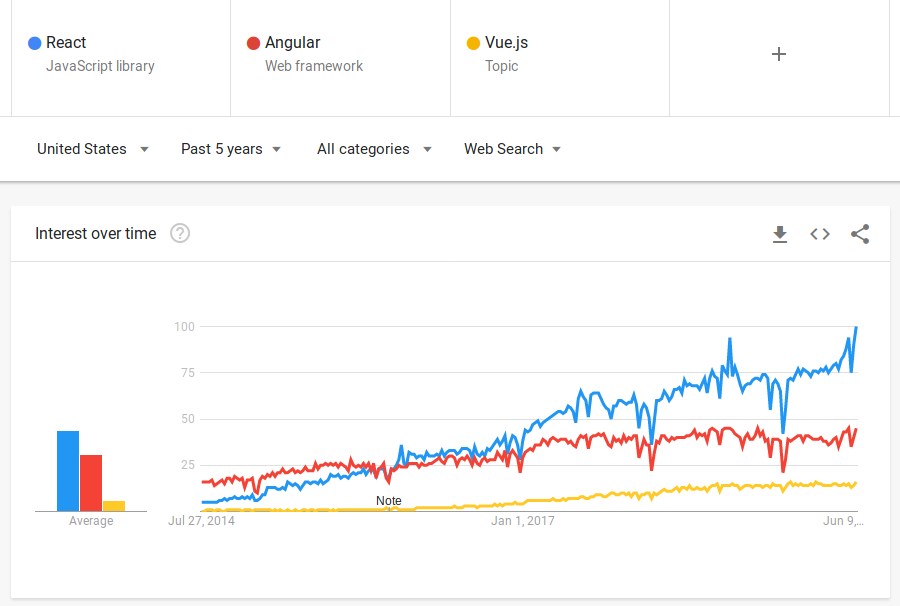
\includegraphics{images/organizational-project-skill-demand_google-trends.png}

ThoughtWorks publishes a series called 'Tech Radar' that shows the
popularity of technologies.

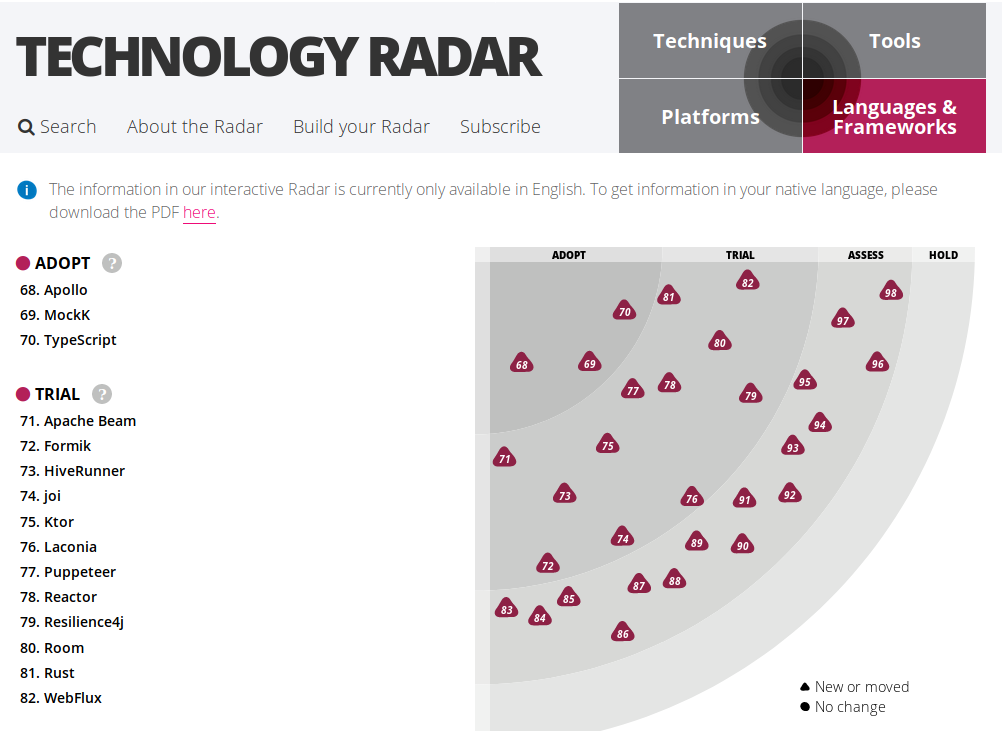
\includegraphics{images/organizational-project-skill-demand_tech-radar.png}

Tech Radar allows you to drill down on projects to see how the
assessment has changed over time.

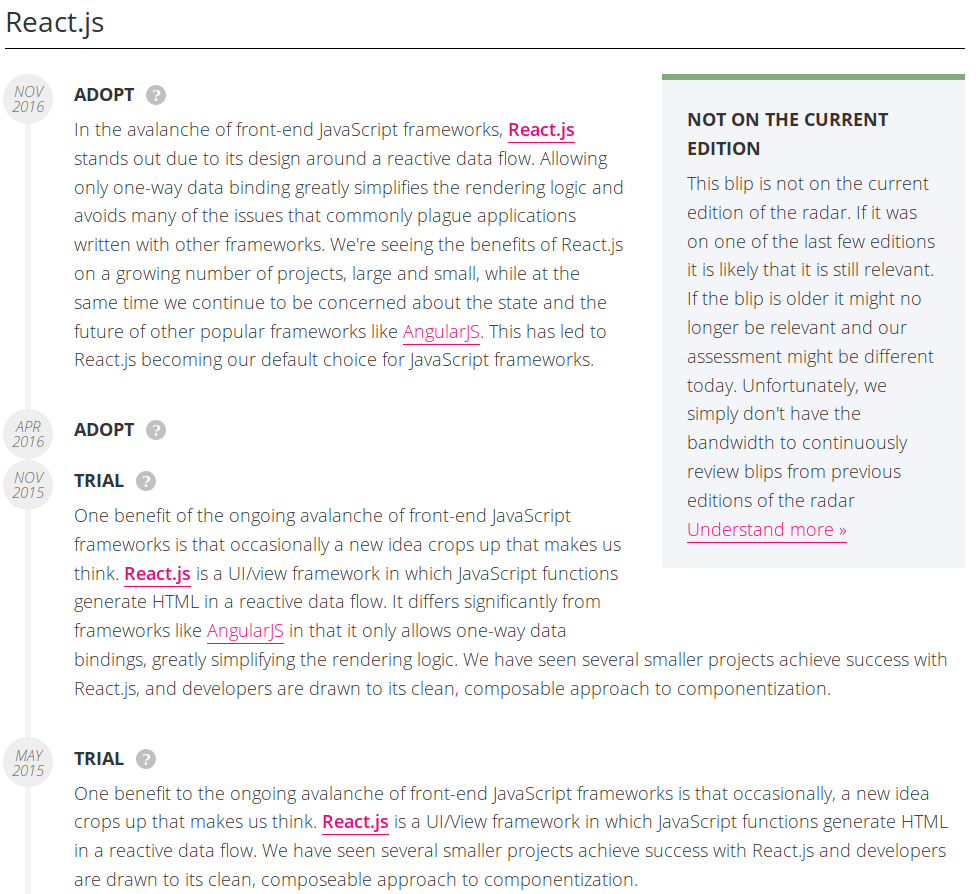
\includegraphics{images/organizational-project-skill-demand_tech-react.png}

StackOverview publishes an annual developer's survey

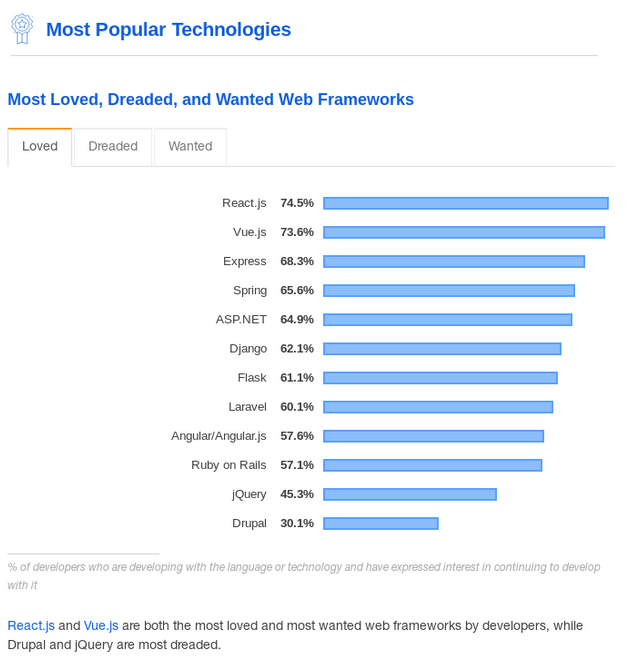
\includegraphics{images/organizational-project-skill-demand_stack-overflow.png}

\hypertarget{tools-providing-the-metric}{%
\subsubsection{Tools Providing the
Metric}\label{tools-providing-the-metric}}

\begin{itemize}
\tightlist
\item
  Google Trends - for showing search interest over time
\item
  ThoughtWorks TechRadar - project assessments from a tech consultancy
\item
  StackOverflow Developer's Survey - annual project rankings
\item
  Augur; Examples are available for multiple repositories:

  \begin{itemize}
  \tightlist
  \item
    \href{http://augur.osshealth.io/repo/Rails\%20(wg-value)/rails/overview}{Rails}
  \item
    \href{http://augur.osshealth.io/repo/Zephyr-RTOS/zephyr/overview}{Zephyr}
  \item
    \href{http://augur.osshealth.io/repo/Apache\%20(wg-value)/cloudstack/overview}{CloudStack}
  \end{itemize}
\end{itemize}

\hypertarget{references}{%
\subsection{References}\label{references}}

\begin{itemize}
\tightlist
\item
  \href{https://opensource.org/sponsors}{Open Source Sponsors}
\item
  \href{https://opensource.com/article/19/1/fiscal-sponsors-open-source}{Fiscal
  Sponsors and Open Source}
\item
  \href{https://www.networkworld.com/article/2867020/big-names-like-google-dominate-open-source-funding.html}{Large
  Corporate OpenSource Sponsors}
\item
  \href{https://www.npmjs.com/package/google-trends-api}{Google Trends
  API}
\item
  \href{https://aisel.aisnet.org/cgi/viewcontent.cgi?article=1496\&context=amcis2018}{Measuring
  Open Source Software Impact}
\item
  \href{https://www.thoughtworks.com/radar}{ThoughtWorks Tech Radar}
\item
  \href{https://insights.stackoverflow.com/survey/2019\#technology}{Stack
  Overflow Developer's Survey}
\end{itemize}
 
 

\subsection{Focus Area - Organizational Value}
\textbf{Goal:} Identify if a project is monetarily valuable from an organization's perspective.
\begin{table}[ht!]
    \centering
    \begin{tabular}{|p{0.35\linewidth} | p{0.6\linewidth}|}
        \hline
        \hfil \textbf{Metric}  & \hfil \textbf{Question} \\
        \hline
    		Labor Investment & What was the cost of an organization for its employees to create the counted contributions (e.g., commits, issues, and pull requests)? \\ 
		\hline
    \end{tabular}
\end{table}
    
\hypertarget{ux4ebaux529bux6295ux8d44}{%
\subsubsection{人力投资}\label{ux4ebaux529bux6295ux8d44}}

问题:组织投入人力对社区所做的贡献(例如:代码提交,议题和更改请求)花费的成本是多少

\hypertarget{ux63cfux8ff0}{%
\paragraph{描述}\label{ux63cfux8ff0}}

开源项目通常由组织的人力投入来支撑。该指标跟踪组织对单个项目的经济投入(体现在人力成本)。

\hypertarget{ux76eeux6807}{%
\paragraph{目标}\label{ux76eeux6807}}

随着组织参与度对开源项目变得越来越重要,组织必须清楚了解其人力投资。该指标的目的是为从事开源项目的组织提高人力成本的透明度。该指标给开源项目办公室(OSPO)经理提供了一种通过项目投资组合比较人力成本的方法。比如:人力投资指标能用在确定投资的优先顺序或者确定投资回报。例如:

\begin{itemize}
\tightlist
\item
  以人力投资评估 OSPO 事务的优先级和证明预算合理性
\item
  以人力投资解释产品、项目管理事项的优先级
\item
  以人力投资论证继续投资 OSPO 的价值
\item
  以人力投资反应和比较开源贡献与内部工作的人力成本
\item
  以人力投资比较项目组合的项目效益
\end{itemize}

\hypertarget{ux5b9eux73b0}{%
\paragraph{实现}\label{ux5b9eux73b0}}

基础指标包括:

\begin{itemize}
\tightlist
\item
  贡献数量
\item
  按贡献者类型(内部/外部)划分的贡献数量
\item
  按贡献类型(如代码提交,议题和更改请求)划分的贡献数量
\end{itemize}

参数包括:

\begin{itemize}
\tightlist
\item
  每小时劳动率
\item
  创建贡献的平均劳动时间(按照贡献类型分类)
\end{itemize}

人力投资 = 每一种贡献类型的总和(贡献数量 * 创造贡献的平均工时 *
平均每小时劳动率)

\hypertarget{ux7b5bux9009ux6761ux4ef6}{%
\subparagraph{筛选条件}\label{ux7b5bux9009ux6761ux4ef6}}

\begin{itemize}
\tightlist
\item
  内部与外部贡献者
\item
  问题标签
\item
  项目来源(如内部、开源仓库、竞争对手的开源仓库)
\end{itemize}

\hypertarget{ux53efux89c6ux5316ux6548ux679c}{%
\subparagraph{可视化效果}\label{ux53efux89c6ux5316ux6548ux679c}}

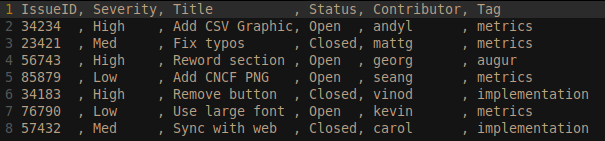
\includegraphics{images/labor-investment_csv.png}

我们的第一个参数化指标的可视化效果依赖于可以用Augur导出的CSV。电子表格用于指标参数和计算公式。未来的实现可能会在
webapp 中直接添加参数操作的功能。

\hypertarget{ux53c2ux8003ux8d44ux6599}{%
\paragraph{参考资料}\label{ux53c2ux8003ux8d44ux6599}}

\begin{itemize}
\tightlist
\item
  \href{https://www.slideshare.net/caniszczyk/starting-an-open-source-program-office-ospo}{启动开源项目办公室}
\item
  \href{https://events19.linuxfoundation.org/wp-content/uploads/2018/07/OSLS_2019-untold-story-of-OSPO.pdf}{创办开源项目办公室}
\item
  \href{https://d1.awsstatic.com/Open\%20Source/enterprise-oss-book.pdf}{企业开源}
\end{itemize}
 
 
 

\end{document}

\section{Common Metrics WG}
\clearpage

\hypertarget{technical-fork}{%
\subsubsection{Technical Fork}\label{technical-fork}}

Question: What are a number of technical forks of an open source project
on code development platforms?

\hypertarget{description}{%
\paragraph{Description}\label{description}}

A technical fork is a distributed version control copy of a project. The
number of technical forks indicates the number of copies of a project on
the same code development platform.

\hypertarget{objectives}{%
\paragraph{Objectives}\label{objectives}}

The objective of the Technical Fork metric is to ascertain how many
copies of a project exist on a code development platform. Analysis of
technical forks may provide insight into forking intentions (different
types of forks such as contributing, and non-contributing forks).

\hypertarget{implementation}{%
\paragraph{Implementation}\label{implementation}}

\hypertarget{filters}{%
\subparagraph{Filters}\label{filters}}

\begin{itemize}
\tightlist
\item
  Time Period (e.g., Weekly, Monthly, Annually)
\item
  Ratio of contributing fork to total forks (A contributing fork is a
  fork that has opened a change request against the original
  repository.)
\item
  Ratio of non-contributing fork to total forks (A non-contributing fork
  is a fork that has never opened a change request against the original
  repository.)
\end{itemize}

\hypertarget{visualizations}{%
\subparagraph{Visualizations}\label{visualizations}}

\textbf{Augur Implementation}\\
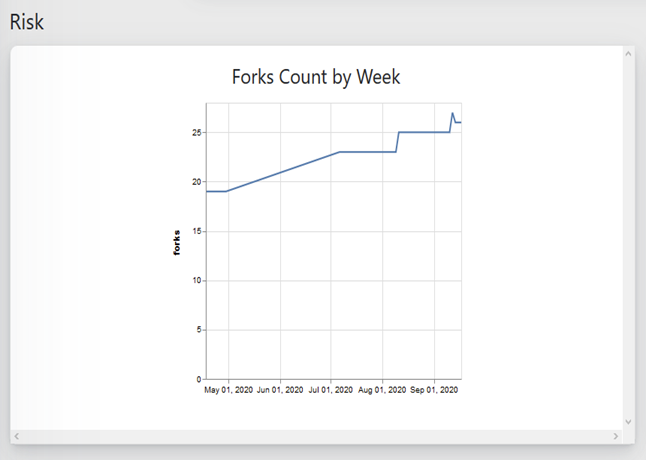
\includegraphics{images/technical-fork_augur-fork.png}

\textbf{GrimoireLab Implementation}\\
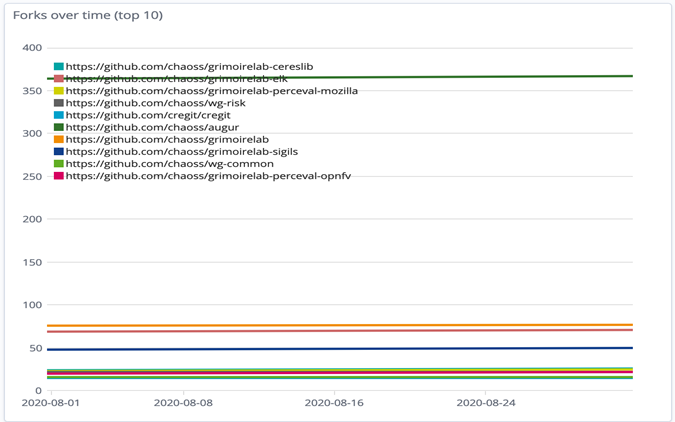
\includegraphics{images/technical-fork_grimoirelab-fork.png}

\hypertarget{tools-providing-the-metric}{%
\subparagraph{Tools Providing the
Metric}\label{tools-providing-the-metric}}

\begin{itemize}
\tightlist
\item
  Augur
\item
  GrimoireLab
\end{itemize}

\hypertarget{data-collection-strategies}{%
\subparagraph{Data Collection
Strategies}\label{data-collection-strategies}}

\textbf{Github API}\\
\url{https://developer.github.com/v3/repos/forks/\#list-forks}

\textbf{GitLab API}\\
\url{https://docs.gitlab.com/ee/api/projects.html\#list-forks-of-a-project}

\textbf{Bitbucket API}\\
\url{https://developer.atlassian.com/bitbucket/api/2/reference/resource/repositories/\%7Bworkspace\%7D/\%7Brepo_slug\%7D/forks}

\hypertarget{references}{%
\paragraph{References}\label{references}}

\url{https://help.github.com/en/enterprise/2.13/user/articles/fork-a-repo}
\url{https://opensource.com/article/17/12/fork-clone-difference}
 
\hypertarget{ux8d21ux732eux7c7bux578b}{%
\subsubsection{贡献类型}\label{ux8d21ux732eux7c7bux578b}}

问题:正在进行哪些类型的贡献?

\hypertarget{ux63cfux8ff0}{%
\paragraph{描述}\label{ux63cfux8ff0}}

多元化的贡献能够使开源项目健康发展。在很多项目中,有些社区成员并不编写代码,但他们同样做出了有价值的贡献,比如管理社区、区分错误、宣传项目、支持用户或以其他方式提供帮助。

\hypertarget{ux76eeux6807}{%
\paragraph{目标}\label{ux76eeux6807}}

多样的贡献类型表明项目是成熟全面的,包含足够的活动来支持项目的所有方面,并且提供多种贡献类型的晋升渠道,让拥有编码之外的不同专长的人员也能够发展到领导层。

\hypertarget{ux5b9eux73b0}{%
\paragraph{实现}\label{ux5b9eux73b0}}

如何对贡献进行定义、量化、跟踪和公布是一个具有挑战性的问题。
每个项目的答案可能都是独一无二的,以下建议仅作为抛砖引玉。作为一个通用指南,很难将不同的贡献类型相互比较,应单独考量。

\begin{itemize}
\tightlist
\item
  以下列表可以帮助确定贡献类型:

  \begin{itemize}
  \tightlist
  \item
    编写代码
  \item
    审查代码
  \item
    错误分类
  \item
    质量保证和测试
  \item
    安全相关活动
  \item
    本地化和翻译
  \item
    事件组织
  \item
    文档编写
  \item
    社区建设和管理
  \item
    教学和教程构建
  \item
    故障排除和支持
  \item
    创意作品和设计
  \item
    用户界面、用户体验和易用性
  \item
    社交媒体管理
  \item
    用户支持和问题解答
  \item
    撰写文章
  \item
    公共关系 - 技术媒体采访
  \item
    事件发言
  \item
    营销与活动宣传
  \item
    网站开发
  \item
    法律委员会
  \item
    财务管理
  \end{itemize}
\end{itemize}

\hypertarget{ux6570ux636eux6536ux96c6ux7b56ux7565}{%
\subparagraph{数据收集策略}\label{ux6570ux636eux6536ux96c6ux7b56ux7565}}

\begin{itemize}
\item
  **采访或调查:**让社区成员认可他人的贡献,找出过去没有考虑到的贡献类型。

  \begin{itemize}
  \tightlist
  \item
    您想表彰谁在项目中的贡献? 他们贡献了什么?
  \end{itemize}
\item
  **观察项目:**找出和认可项目不同部分的负责人。

  \begin{itemize}
  \tightlist
  \item
    在项目网站或代码仓库中列出了哪些负责人?
  \end{itemize}
\item
  **捕获非代码贡献:**通过问题跟踪器等专用系统跟踪贡献。

  \begin{itemize}
  \tightlist
  \item
    日志记录可以包含项目要了解的关于非代码贡献的定制化信息,用以识别工作量。
  \item
    通过沟通渠道活动的代理贡献。 例如,如果质量保证成员 (QA)
    拥有自己的邮件列表,就可以通过邮件列表活动来代理衡量围绕 QA
    贡献的活动。
  \end{itemize}
\item
  **收集跟踪数据:**通过协作工具日志数据衡量贡献。

  \begin{itemize}
  \tightlist
  \item
    例如,可以从源代码仓库计算代码贡献,可以从维基编辑历史记录计算维基贡献,可以从电子邮件归档计算电子邮件消息
  \end{itemize}
\item
  **自动分类:**训练人工智能 (AI) 机器人来检测贡献并对其分类。

  \begin{itemize}
  \tightlist
  \item
    AI
    机器人可以协助对贡献进行分类,例如,帮助请求与提供的支持,或功能请求与错误报告,尤其是以上均在同一个问题跟踪器中完成的情况。
  \end{itemize}
\end{itemize}

\emph{其他考量:}

\begin{itemize}
\tightlist
\item
  特别是对于自动报告,允许社区成员选择退出并不出现在贡献报告上。
\item
  承认对贡献类型的捕捉不完善,并明确说明收集了哪些类型的贡献。
\item
  随着项目发展,贡献类型的收集方法需要作出调整。
  例如,交换国际化库时,围绕本地化的项目活动可能会在变化前后产生不同的指标。
\item
  大规模挖掘贡献类型时,要考虑机器人的活动。
\end{itemize}

\hypertarget{ux53c2ux8003ux8d44ux6599}{%
\paragraph{参考资料}\label{ux53c2ux8003ux8d44ux6599}}

\begin{itemize}
\tightlist
\item
  \href{https://medium.com/@sunnydeveloper/revisiting-the-word-recognition-in-foss-and-the-dream-of-open-credentials-d15385d49447}{https://medium.com/@sunnydeveloper/revisiting-the-word-recognition-in-foss-and-the-dream-of-open-credentials-d15385d49447}
\item
  \href{https://24pullrequests.com/contributing}{https://24pullrequests.com/contributing}
\item
  \href{https://smartbear.com/blog/test-and-monitor/14-ways-to-contribute-to-open-source-without-being/}{https://smartbear.com/blog/test-and-monitor/14-ways-to-contribute-to-open-source-without-being/}
\item
  \href{https://wiki.openstack.org/wiki/AUCRecognition}{https://wiki.openstack.org/wiki/AUCRecognition}
\item
  \href{https://www.drupal.org/drupalorg/blog/a-guide-to-issue-credits-and-the-drupal.org-marketplace}{https://www.drupal.org/drupalorg/blog/a-guide-to-issue-credits-and-the-drupal.org-marketplace}
\end{itemize}
 
 

\subsection{Focus Area - When}
\textbf{Goal:} Understand when contributions from organizations and people are happening.
\begin{table}[ht!]
    \centering
    \begin{tabular}{|p{0.35\linewidth} | p{0.6\linewidth}|}
        \hline
        \hfil \textbf{Metric}  & \hfil \textbf{Question} \\
        \hline
		Activity Dates and Times & What are the dates and timestamps of when contributor activities occur? \\ 
		\hline
		Burstiness & How are short timeframes of intense activity, followed by a corresponding return to a typical pattern of activity, observed in a project? \\ 
		\hline
		Review Cycle Duration within a Change Request & What is the duration of a review cycle within a single change request? \\ 
		\hline
		Time to Close & How much time passes between creating and closing an operation such as an issue, change request, or support ticket? \\ 
		\hline
		Time to First Response & How much time passes between when an activity requiring attention is created and the first response? \\ 
		\hline
    \end{tabular}
\end{table}

\hypertarget{activity-dates-and-times}{%
\section{Activity Dates and Times}\label{activity-dates-and-times}}

Question: What are the dates and timestamps of when contributor
activities occur?

\hypertarget{description}{%
\subsection{Description}\label{description}}

Individuals engage in activities in open source projects at various
times of the day. This metric is aimed at determining the dates and
times of when individual activities were completed. The data can be used
to probabilistically estimate where on earth contributions come from in
cases where the time zone is not UTC.

\hypertarget{objectives}{%
\subsection{Objectives}\label{objectives}}

\begin{itemize}
\tightlist
\item
  Improve transparency for employers about when organizational employees
  are engaging with open source projects
\item
  Improve transparency for open source project and community managers as
  to when activity is occurring
\end{itemize}

\hypertarget{implementation}{%
\subsection{Implementation}\label{implementation}}

\hypertarget{filters}{%
\subsubsection{Filters}\label{filters}}

\begin{itemize}
\tightlist
\item
  Individual by Organization
\item
  Aggregation of time by UTC time

  \begin{itemize}
  \tightlist
  \item
    Can show what times across the globe contributions are made; when
    the project is most active.
  \end{itemize}
\item
  Aggregation of time by local time

  \begin{itemize}
  \tightlist
  \item
    Can show what times of day in their local times they contribute.
    Conclusions about the If contributions are more during working
    hours, or if contributions are more during evening hours.
  \end{itemize}
\item
  Repository ID
\item
  Segment of a community, (e.g., GrimoireLab has more EU time zones
  activity and Augur more US time zones activity)
\end{itemize}

\hypertarget{visualizations}{%
\subsubsection{Visualizations}\label{visualizations}}

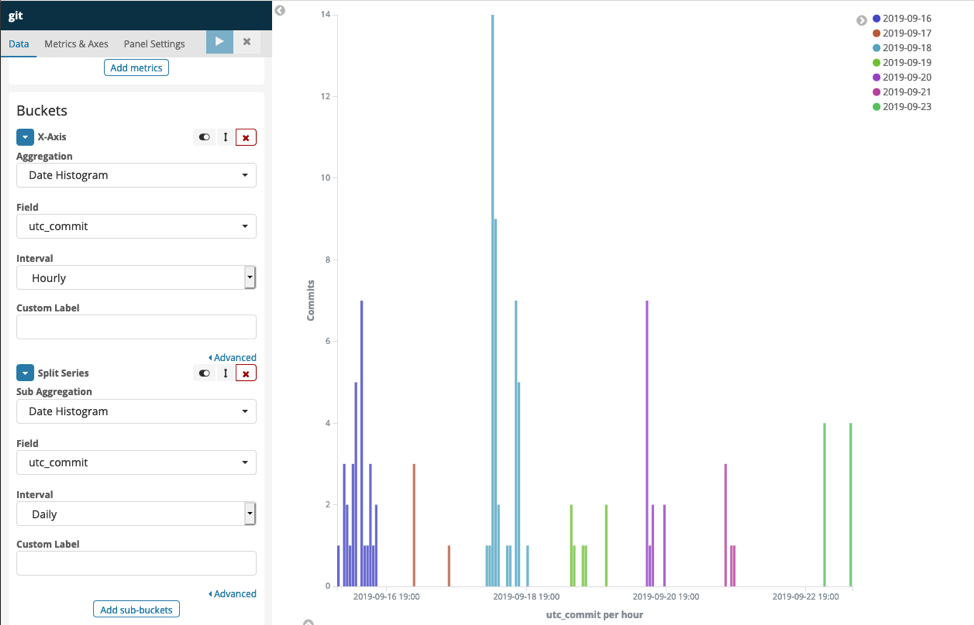
\includegraphics{images/activity-dates-and-times_1.png}
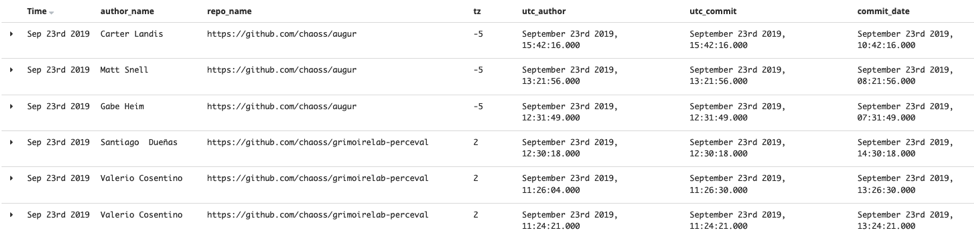
\includegraphics{images/activity-dates-and-times_2.png}
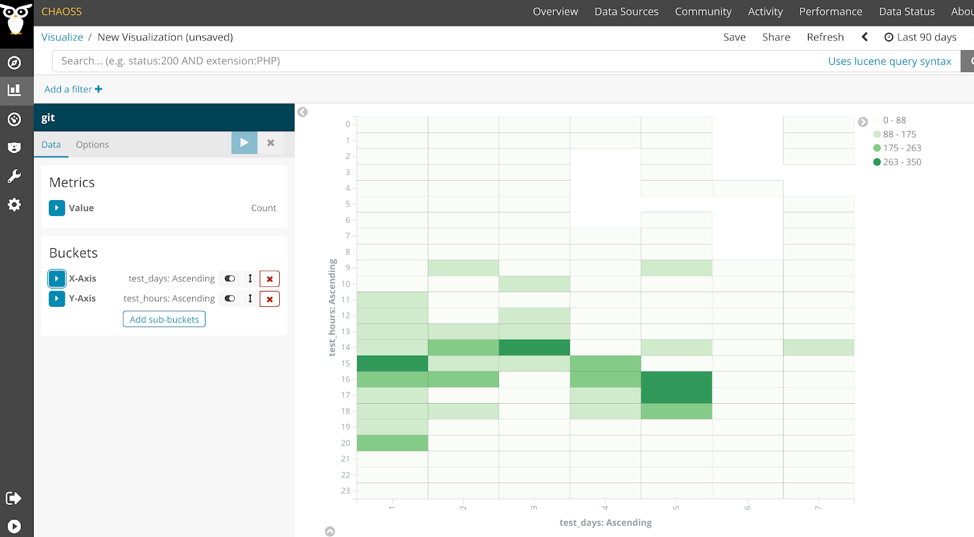
\includegraphics{images/activity-dates-and-times_3.png}
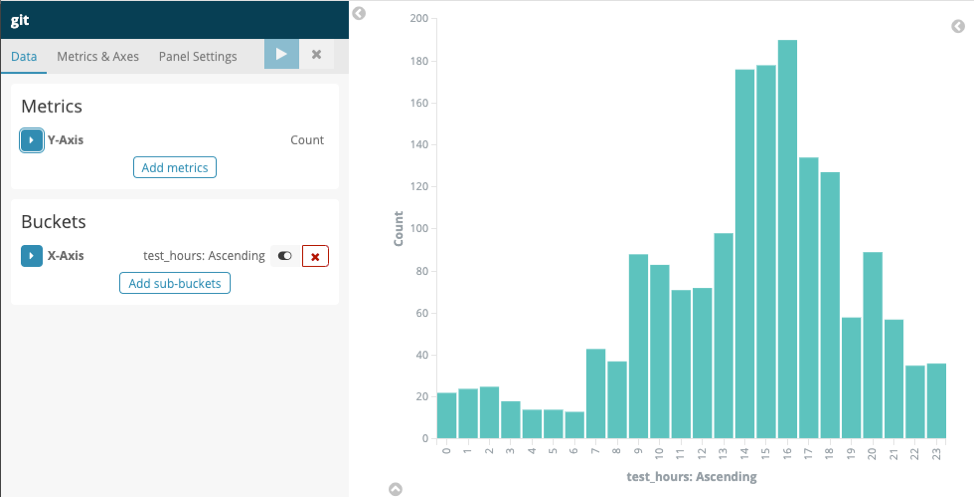
\includegraphics{images/activity-dates-and-times_4.png}

\hypertarget{tools-providing-metric}{%
\subsubsection{Tools Providing Metric}\label{tools-providing-metric}}

\href{https://chaoss.github.io/grimoirelab/}{GrimoireLab}

\href{https://docs.augur.net/\#dates-timestamps}{Augur Date/Timestamps}

\hypertarget{references}{%
\subsection{References}\label{references}}

\href{https://en.wikipedia.org/wiki/Coordinated_Universal_Time}{Coordinated
Universal Time}
 
\hypertarget{burstiness}{%
\section{Burstiness}\label{burstiness}}

Question: How are short timeframes of intense activity, followed by a
corresponding return to a typical pattern of activity, observed in a
project?

\hypertarget{description}{%
\subsection{Description}\label{description}}

There are a number of reasons that may prompt a sudden increase or
decrease in the amount of activity within a repository. These increases
and decreases appear both as a sudden change in activity against the
average amount of activity. Burstiness is a way of understanding the
cycle of activity in existing metrics, like issues, merge requests,
mailing lists, commits, or comments. Examples of root causes for bursts
in activity include:

\begin{itemize}
\tightlist
\item
  Release cycles
\item
  Global pandemics
\item
  Hackathon activities
\item
  Mentorship programs
\item
  Conferences, meetups, and other events where tools are presented
\item
  Conventional and social media announcements and mentions
\item
  Critical bugs as raising awareness and getting people's attention
\item
  Community design meetings or brainstorming meetings to address a
  particular issue
\item
  Community members show up from another community that is relying on
  your project (e.g., dependencies)
\end{itemize}

\hypertarget{objectives}{%
\subsection{Objectives}\label{objectives}}

\begin{itemize}
\tightlist
\item
  To identify impacts of root causes of a burst in activity
\item
  To provide awareness when project activity unknowingly goes up
\item
  To help capture the meaningfulness of increases or decreases in
  project activity
\item
  To help the community and maintainers prepare for future bursts that
  follow a pattern
\item
  To help measure the impact of influential external activities
\item
  To differentiate skewed activity versus normal activity
\end{itemize}

\hypertarget{implementation}{%
\subsection{Implementation}\label{implementation}}

\hypertarget{filters}{%
\subsubsection{Filters}\label{filters}}

\begin{itemize}
\tightlist
\item
  Stars
\item
  Forks
\item
  Issues or bug reports
\item
  Labels
\item
  Downloads
\item
  Release Tags
\item
  Change Requests
\item
  Mail List Traffic
\item
  Documentation additions or revisions
\item
  New Repositories
\item
  Feature Requests
\item
  Messaging Conversations
\item
  Conventional and Social Media Activity
\item
  Conference Attendance and Submissions
\end{itemize}

\hypertarget{visualizations}{%
\subsubsection{Visualizations}\label{visualizations}}

Augur:

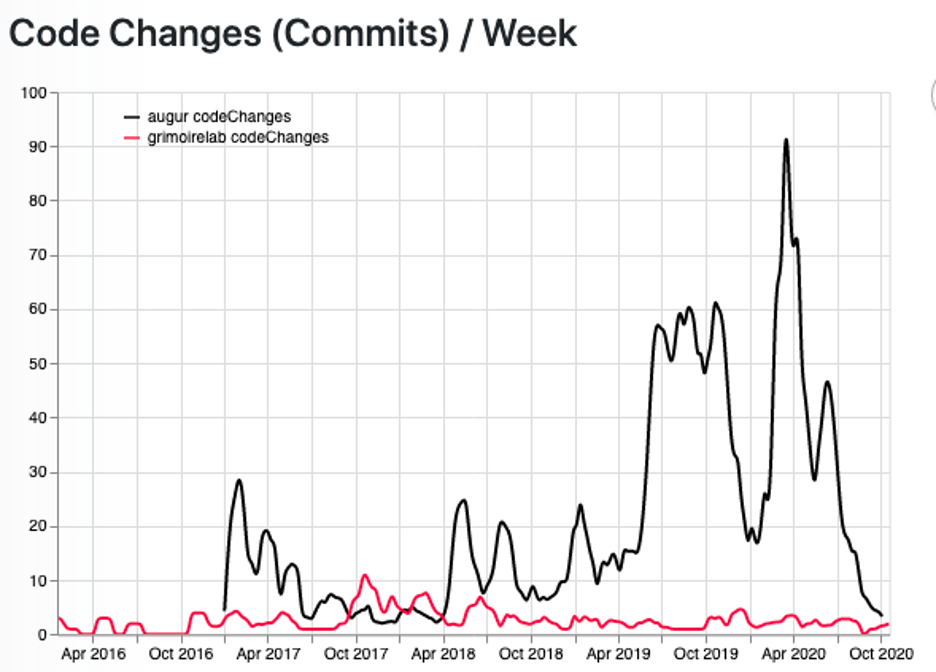
\includegraphics{images/burstiness_augur.png}

GrimoireLab:

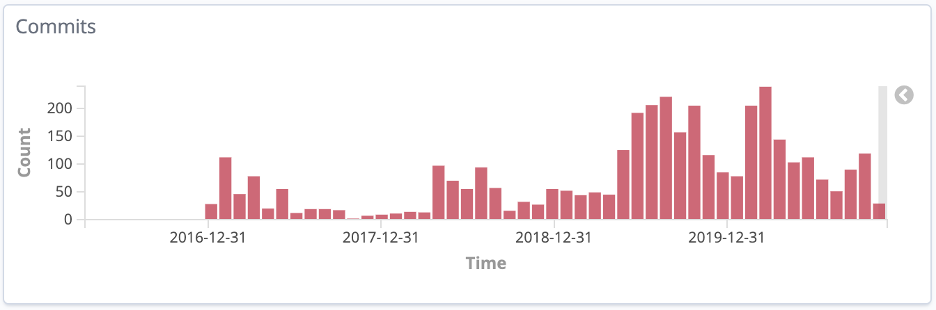
\includegraphics{images/burstiness_gl.png}

\hypertarget{tools-providing-the-metric}{%
\subsubsection{Tools Providing the
Metric}\label{tools-providing-the-metric}}

\begin{itemize}
\tightlist
\item
  Grimoire Lab
\item
  Augur
\end{itemize}

\hypertarget{data-collection-strategies}{%
\subsubsection{Data Collection
Strategies}\label{data-collection-strategies}}

\begin{itemize}
\item
  Quantitative

  \begin{itemize}
  \tightlist
  \item
    Time box activities identifying deviations away from some norm
  \item
    Outliers for certain thresholds, using statistics like Bollinger
    Bands to measure stability or volatility:
    \url{https://en.wikipedia.org/wiki/Bollinger_Bands}
  \end{itemize}
\item
  Qualitative Interview Questions

  \begin{itemize}
  \tightlist
  \item
    Why do you contribute more during a period of time?
  \item
    What do you believe to be the root cause for particular bursts?
  \item
    What impact do different events (e.g., hackathons, mentorship
    program, or conferences) have on project activity?
  \end{itemize}
\end{itemize}

\hypertarget{references}{%
\subsection{References}\label{references}}

This metric was inspired by the work of Goh and Barabasi (2008):
\url{https://arxiv.org/pdf/physics/0610233.pdf}
 
\hypertarget{review-cycle-duration-within-a-change-request}{%
\subsubsection{Review Cycle Duration within a Change
Request}\label{review-cycle-duration-within-a-change-request}}

Question: What is the duration of a review cycle within a single change
request?

\hypertarget{description}{%
\paragraph{Description}\label{description}}

A change request is based on one or more review cycles. Within a review
cycle, one or more reviewers can provide feedback on a proposed
contribution. The duration of a review cycle, or the time between each
new iteration of the contribution, is the basis of this metric.

\hypertarget{objectives}{%
\paragraph{Objectives}\label{objectives}}

This metric provides maintainers with insight on: Code review process
decay, as there are more iterations and review cycle durations increase.
Process bottlenecks resulting in long code review iterations. Abandoned
or semi-abandoned processes in the review cycles, where either the
maintainer or the submitter is slow in responding. Characteristics of
reviews that have different cyclic pattern lengths.

\hypertarget{implementation}{%
\paragraph{Implementation}\label{implementation}}

Review Cycle Duration is measured as the time length of one review cycle
within a single change request. The duration can be calculated between:
The moment when each review cycle begins, defined as the point in time
when a change request is submitted or updated. The moment when each
review cycle ends, either because the change request was updated and
needs a new review or because it was accepted or rejected.

\hypertarget{filter}{%
\subparagraph{Filter}\label{filter}}

Average or Median Duration, optionally filtered or grouped by: Number of
people involved in review Number of comments in review Edits made to a
change request Project or program Organization making the change request
Time the change request was submitted Developers who contributed to a
change request Change request Number of review cycle on a change request
(e.g., filter by first, second, \ldots{} round)

\hypertarget{visualizations}{%
\subparagraph{Visualizations}\label{visualizations}}

\hypertarget{tools-providing-the-metric}{%
\subparagraph{Tools Providing the
Metric}\label{tools-providing-the-metric}}

\hypertarget{references}{%
\paragraph{References}\label{references}}

Example of data that could be used to develop the metric:
\url{https://gerrit.wikimedia.org/r/c/mediawiki/core/+/194071}
 
\hypertarget{ux5173ux95edux65f6ux957f}{%
\subsubsection{关闭时长}\label{ux5173ux95edux65f6ux957f}}

问题:创建和关闭操作(如议题、更改请求或需要支持的问题单)之间需要多少时间?

\hypertarget{ux63cfux8ff0}{%
\paragraph{描述}\label{ux63cfux8ff0}}

关闭时长是指从创建到关闭操作(如议题、更改请求或需要支持的问题单)的总时长。
操作需要具有打开和关闭的状态,比如代码审查进程、问答论坛、问题跟踪系统中经常出现的情况。

相关指标:\href{https://chaoss.community/metric-issue-resolution-duration/}{问题解决时长}

\hypertarget{ux76eeux6807}{%
\paragraph{目标}\label{ux76eeux6807}}

\begin{enumerate}
\def\labelenumi{\arabic{enumi}.}
\tightlist
\item
  确定社区的响应程度,帮助增加包容性,吸引新贡献者并保留现有贡献者。
\item
  找出导致快速或缓慢关闭的操作特征(如寻找最佳实践、改进领域、评估效率)。
\item
  识别对不同社区成员及时响应的偏差。
\item
  检测社区活动的变化(例如,显示潜在的维护者倦怠、贡献多元化的减少)
\item
  了解关闭议题或更改请求的时间与合并成功或失败的关系
\end{enumerate}

\hypertarget{ux5b9eux73b0}{%
\paragraph{实现}\label{ux5b9eux73b0}}

\hypertarget{ux7b5bux9009ux6761ux4ef6}{%
\subparagraph{筛选条件}\label{ux7b5bux9009ux6761ux4ef6}}

\begin{itemize}
\tightlist
\item
  操作的创建者(例如,新贡献者相对于维护者)
\item
  最初关闭,最后关闭
\item
  标签(例如错误与新功能)
\item
  更改请求合并状态(例如,合并时间或没有合并的关闭时间)
\end{itemize}

\hypertarget{ux53efux89c6ux5316ux6548ux679c}{%
\subparagraph{可视化效果}\label{ux53efux89c6ux5316ux6548ux679c}}

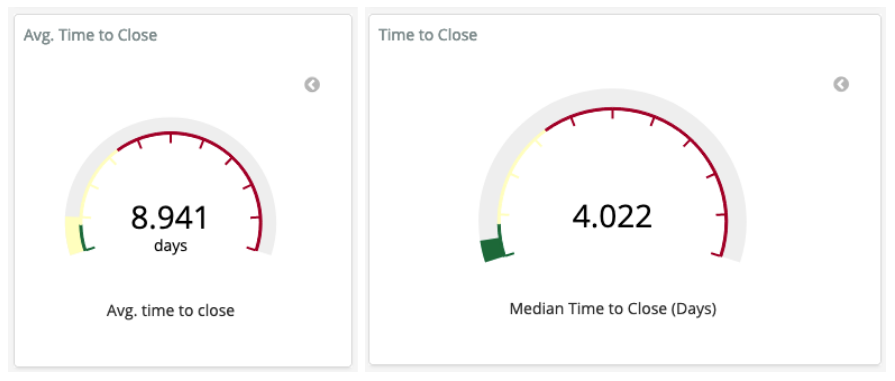
\includegraphics{images/time-to-close_1.png}

\hypertarget{ux63d0ux4f9bux6307ux6807ux7684ux5de5ux5177}{%
\subparagraph{提供指标的工具}\label{ux63d0ux4f9bux6307ux6807ux7684ux5de5ux5177}}

Augur 实现:

\begin{itemize}
\tightlist
\item
  \href{http://augur.osshealth.io/api_docs/\#api-Evolution-Closed_Issue_Resolution_Duration(Repo)}{问题解决时长}
\item
  \href{http://augur.osshealth.io/api_docs/\#api-Evolution-issue-duration-repo}{问题持续时间}
\item
  \href{http://augur.osshealth.io/api_docs/\#api-Evolution-Issue_Response_Time(Repo)}{问题响应时间}
\end{itemize}

GrimoireLab 实现:

\begin{itemize}
\tightlist
\item
  \href{https://chaoss.github.io/grimoirelab-sigils/panels/github-pullrequests-efficiency/}{拉取请求效率}
\item
  \href{https://chaoss.github.io/grimoirelab-sigils/panels/github-issues-efficiency/}{问题效率}
\item
  \href{https://chaoss.github.io/grimoirelab-sigils/panels/efficiency-timing-overview/}{Efficiency:TimingOverview}
\end{itemize}

\hypertarget{ux6570ux636eux6536ux96c6ux7b56ux7565}{%
\subparagraph{数据收集策略}\label{ux6570ux636eux6536ux96c6ux7b56ux7565}}

关闭时长指标可根据项目活动和目标的具体情况而定。
例如,错误报告的关闭时长可能提供与新功能请求的关闭时长不同的信息。
数据收集策略应针对不同的项目目标。 可能影响这些进程的其他变量是:

\begin{itemize}
\tightlist
\item
  问题跟踪系统:如错误报告、蓝图 (OpenStack 专有命名)、用户故事(user
  story)、功能请求、epic等可能会影响事件关闭时长的议题类型。
  优先级或严重性等其他变量可能有助于推进这一事件的关闭速度。
\item
  变更请求流程:这取决于变更请求的平台架构,如 Gerrit、GitHub
  或邮件列表(如 Linux 内核中),并可能根据进程的复杂程度而有所不同。
  例如,新人和经验丰富的高级开发者将以不同的方式开展进程,所需时间或多或少。
\item
  问答论坛:这取决于回答的质量和提问者的意见。
  有效答案会被标记,提问者成功找到自己问题的正确答案后,进程随即关闭。
\end{itemize}

\hypertarget{ux53c2ux8003ux8d44ux6599}{%
\paragraph{参考资料}\label{ux53c2ux8003ux8d44ux6599}}

\begin{itemize}
\tightlist
\item
  ``Practice P.12: Respond to all submissions'',出自``Appendix to:
  Managing Episodic Volunteers in Free/Libre/Open Source Software
  Communities'',Ann Barcomb、Klaas-Jan Stol、Brian Fitzgerald 和 Dirk
  Riehle:\href{https://opus4.kobv.de/opus4-fau/frontdoor/index/index/docId/13519}{https://opus4.kobv.de/opus4-fau/frontdoor/index/index/docId/13519}
\end{itemize}
 
\hypertarget{time-to-first-response}{%
\subsubsection{Time to First Response}\label{time-to-first-response}}

Question: How much time passes between when an activity requiring
attention is created and the first response?

\hypertarget{description}{%
\paragraph{Description}\label{description}}

The first response to an activity can sometimes be the most important
response. The first response shows that a community is active and
engages in conversations. A long time to respond to an activity can be a
sign that a community is not responsive. A short time to respond to an
activity can help to engage more members into further discussions and
within the community.

\hypertarget{objectives}{%
\paragraph{Objectives}\label{objectives}}

Identify cadence of first response across a variety of activities,
including PRs, Issues, emails, IRC posts, etc. Time to first response is
an important consideration for new and long-time contributors to a
project along with overall project health.

\hypertarget{implementation}{%
\paragraph{Implementation}\label{implementation}}

Time to first response of an activity = time first response was posted
to the activity - time the activity was created.

\hypertarget{filters}{%
\subparagraph{Filters}\label{filters}}

\begin{itemize}
\tightlist
\item
  Role of responder, e.g., only count maintainer responses
\item
  Automated responses, e.g., only count replies from real people by
  filtering bots and other automated replies
\item
  Type of Activity, e.g., issues (see metric
  \href{https://github.com/chaoss/wg-evolution/blob/master/metrics/Issue_Response_Time.md}{Issue
  Response Time}), emails, chat, change requests
\end{itemize}

\hypertarget{visualizations}{%
\subparagraph{Visualizations}\label{visualizations}}

<<<<<<< HEAD
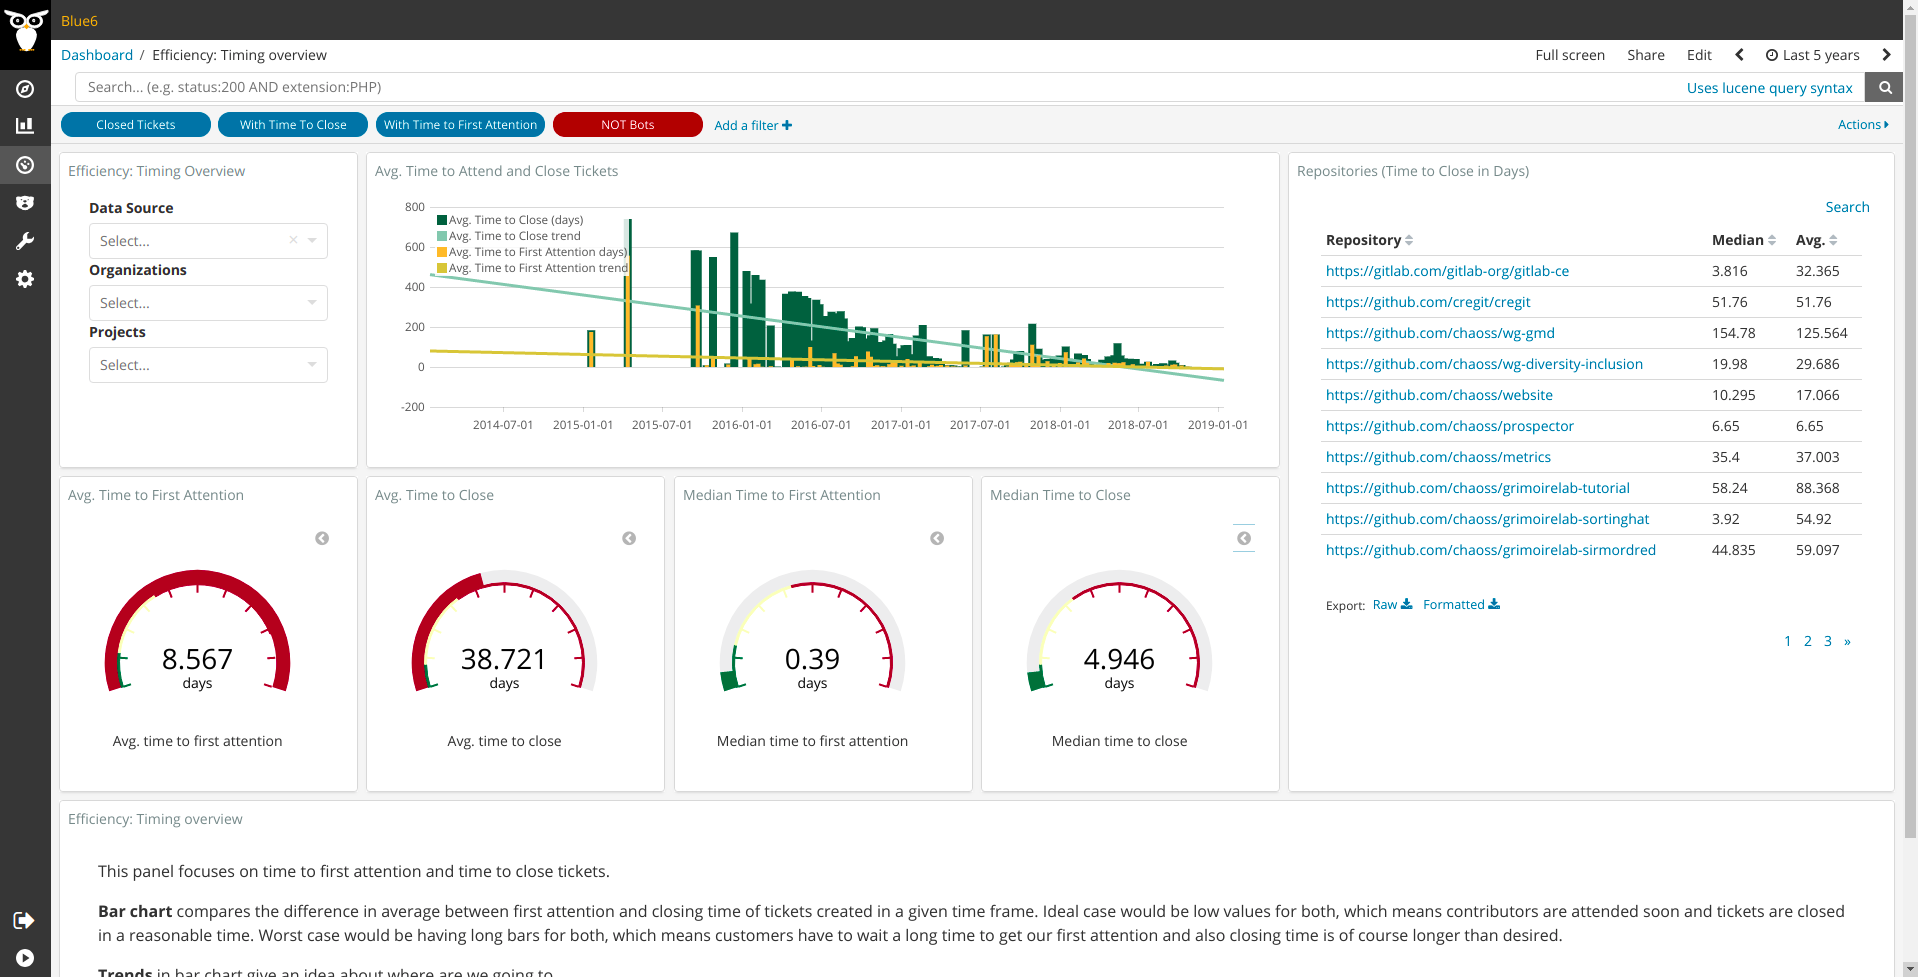
\includegraphics{images/time-to-first-response_efficiency-timing-overview.png}

\begin{center}\rule{0.5\linewidth}{0.5pt}\end{center}

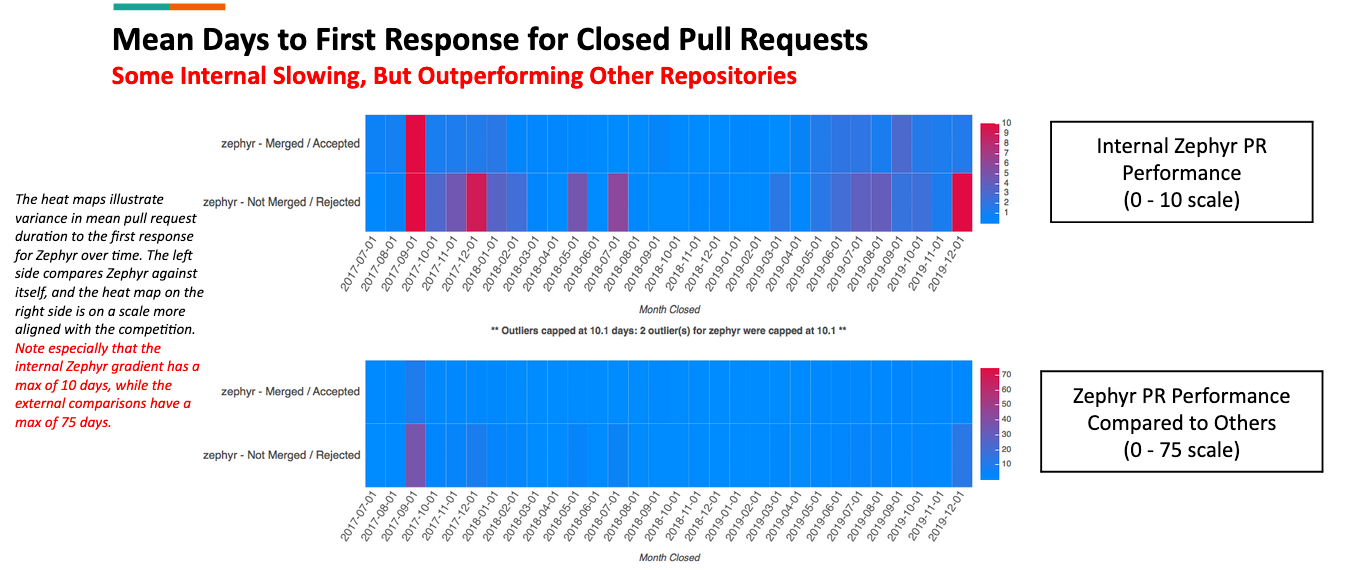
\includegraphics{images/time-to-first-response_augur-ttc-1.png}

\begin{center}\rule{0.5\linewidth}{0.5pt}\end{center}
=======
\hypertarget{grimoirelab-panel-efficiency-timing-overview}{%
\subsection{\texorpdfstring{\protect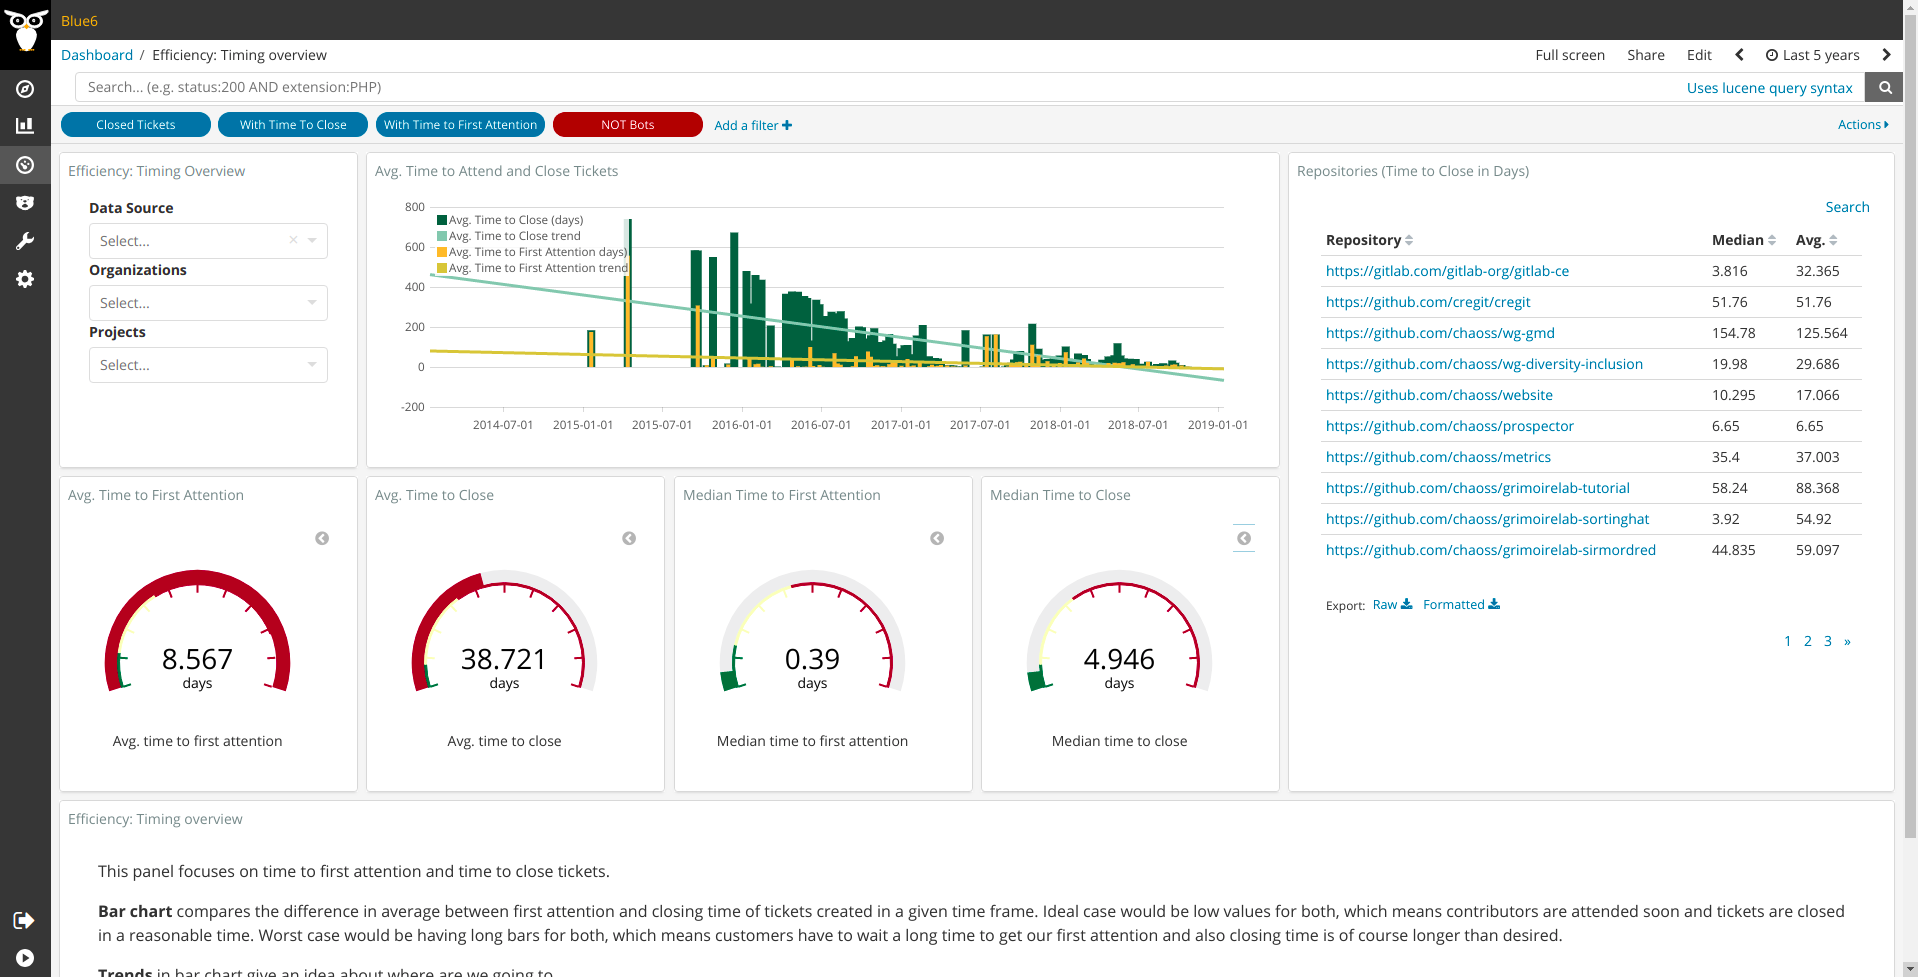
\includegraphics{images/time-to-first-response_efficiency-timing-overview.png}}{GrimoireLab Panel: Efficiency Timing Overview}}\label{grimoirelab-panel-efficiency-timing-overview}}

\hypertarget{augur-visualization-time-to-first-response-heat-map-}{%
\subsection{\texorpdfstring{\protect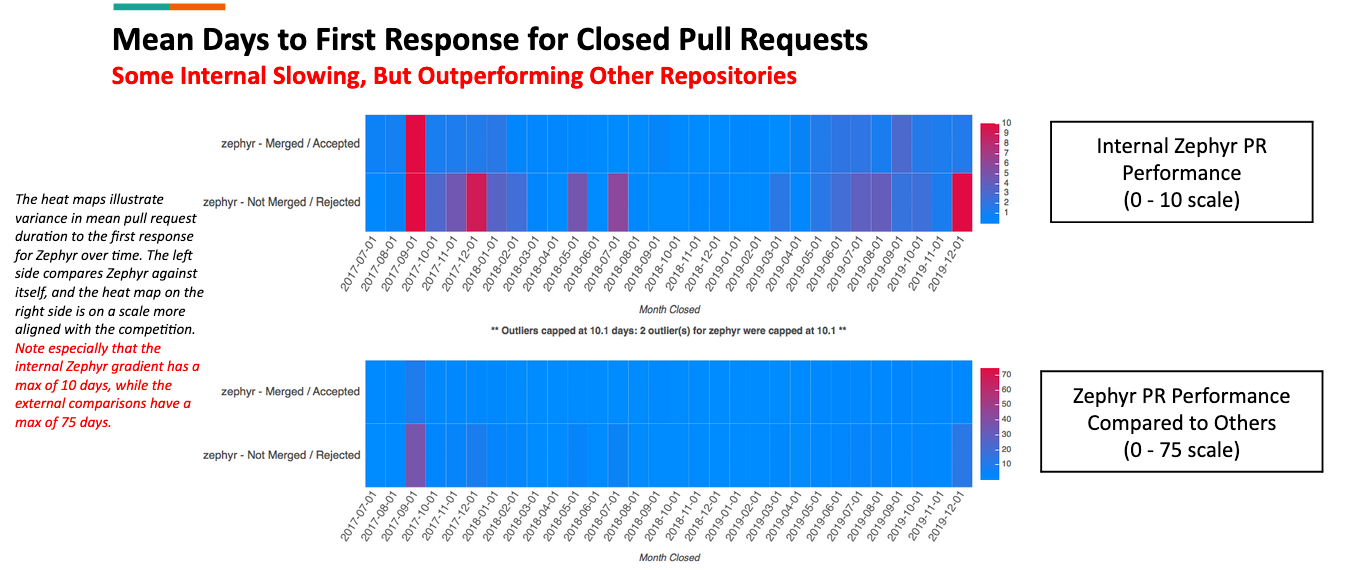
\includegraphics{images/time-to-first-response_augur-ttc-1.png}}{Augur Visualization: Time to First Response Heat Map }}\label{augur-visualization-time-to-first-response-heat-map-}}
>>>>>>> main

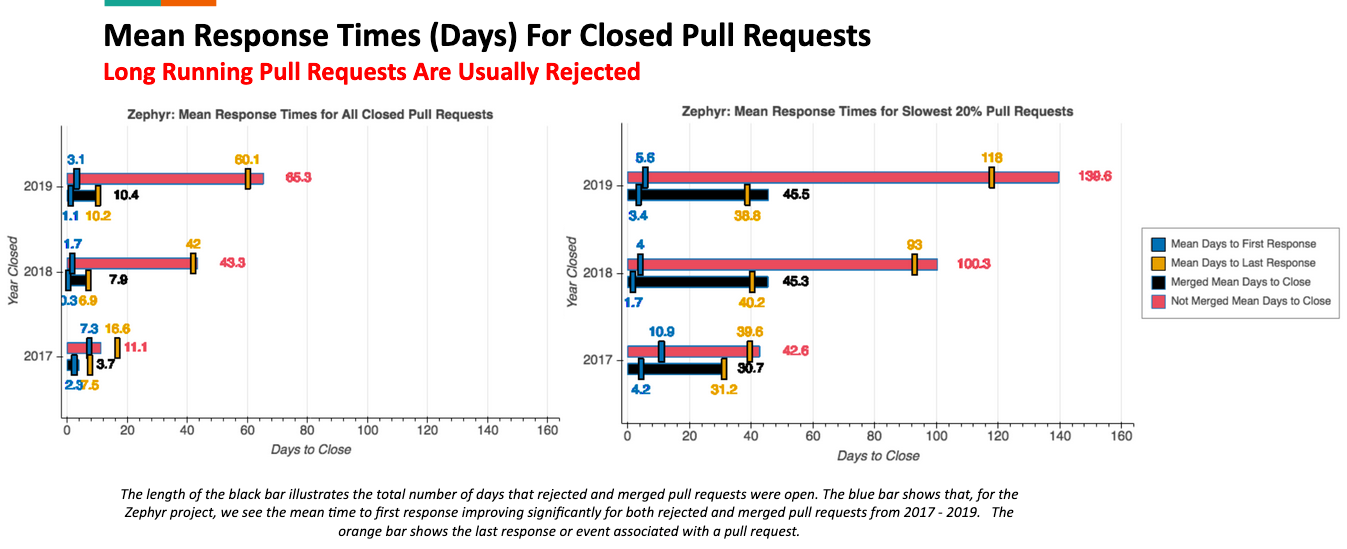
\includegraphics{images/time-to-first-response_augur-ttc-2.png}

\hypertarget{tools-providing-the-metric}{%
\subparagraph{Tools Providing the
Metric}\label{tools-providing-the-metric}}

\begin{itemize}
\tightlist
\item
  GrimoireLab Panel:
  \href{https://chaoss.github.io/grimoirelab-sigils/panels/efficiency-timing-overview/}{Efficiency
  Timing Overview}
\item
  \href{https://katacontainers.biterg.io/app/kibana\#/dashboard/cbbdd920-288c-11e9-b662-975152e57997}{Kata
  Containers dashboard efficiency panel}
\end{itemize}

\hypertarget{references}{%
\paragraph{References}\label{references}}
 
 

\subsection{Focus Area - who}
\textbf{Goal:} Understand organizational and personal engagement with open source projects
\begin{table}[ht!]
    \centering
    \begin{tabular}{|p{0.35\linewidth} | p{0.6\linewidth}|}
        \hline
        \hfil \textbf{Metric}  & \hfil \textbf{Question} \\
        \hline
		Contributor Location & What is the location of contributors? \\ 
		\hline
		Contributors & Who are the contributors to a project? \\ 
		\hline
		Organizational Diversity & What is the organizational diversity of contributions? \\ 
		\hline
    \end{tabular}
\end{table}
 
 


    \section{Value WG}
    \begin{table}[ht!]
        \centering
        \begin{tabular}{|p{0.35\linewidth} | p{0.6\linewidth}|}
            \hline
            \hfil \textbf{关注领域}  & \hfil \textbf{目标} \\
            \hline
        		公共价值 & 确定项目(包括下游项目)是否对社区用户或者贡献者有价值。 \\ 
		\hline
		Placeholder & Placeholder \\ 
		\hline
		人力投资 & 从组织的角度看项目是否具有经济价值。 \\ 
		\hline
    \end{tabular}
    \end{table}
        
\clearpage

    \subsection{关注领域 - 公共价值}
    \textbf{目标:} 确定项目(包括下游项目)是否对社区用户或者贡献者有价值。
    \begin{table}[ht!]
        \centering
        \begin{tabular}{|p{0.35\linewidth} | p{0.6\linewidth}|}
            \hline
            \hfil \textbf{度量指标}  & \hfil \textbf{问题} \\
            \hline
        		项目发展速度 & 如何衡量组织的发展速度? \\ 
		\hline
    \end{tabular}
    \end{table}
        
\hypertarget{project-velocity}{%
\subsubsection{Project Velocity}\label{project-velocity}}

Question: What is the development speed for an organization?

\hypertarget{description}{%
\paragraph{Description}\label{description}}

Project velocity is the number of issues, the number of pull requests,
volume of commits, and number of contributors as an indicator of
'innovation'.

\hypertarget{objectives}{%
\paragraph{Objectives}\label{objectives}}

Gives an Open Source Program Office (OSPO) manager a way to compare the
project velocity across a portfolio of projects.

The OSPO manager can use the Project Velocity metric to:

\begin{itemize}
\tightlist
\item
  Report project velocity of open source projects vs in-house projects
\item
  Compare project velocity across a portfolio of projects
\item
  Identify which projects grow beyond internal contributors (when
  filtering internal vs. external contributors)
\item
  Identify promising areas in which to get involved
\item
  Highlight areas likely to be the successful platforms over the next
  several years
\end{itemize}

\href{https://www.cncf.io/blog/2017/06/05/30-highest-velocity-open-source-projects}{See
Example}

\hypertarget{implementation}{%
\paragraph{Implementation}\label{implementation}}

Base metrics include:

\begin{itemize}
\tightlist
\item
  \href{https://github.com/chaoss/wg-evolution/blob/master/metrics/Issues_Closed.md}{issues
  closed}
\item
  \href{https://github.com/chaoss/wg-evolution/blob/master/metrics/Reviews.md}{number
  of reviews}
\item
  \href{https://github.com/chaoss/wg-evolution/blob/master/metrics/Code_Changes.md}{\#
  of code changes}
\item
  \href{https://github.com/chaoss/wg-risk/blob/master/metrics/Committers.md}{\#
  of committers}
\end{itemize}

\hypertarget{filters}{%
\subparagraph{Filters}\label{filters}}

\begin{itemize}
\tightlist
\item
  Internal vs external contributors
\item
  Project sources (e.g., internal repositories, open-source
  repositories, and competitor open-source repositories)
\item
  Time
\end{itemize}

\hypertarget{visualizations}{%
\subparagraph{Visualizations}\label{visualizations}}

\begin{itemize}
\tightlist
\item
  X-Axis: Logarithmic scale for Code Changes
\item
  Y-Axis: Logarithmic scale of Sum of Number of Issues and Number of
  Reviews
\item
  Dot-size: Committers
\item
  Dots are projects
\end{itemize}

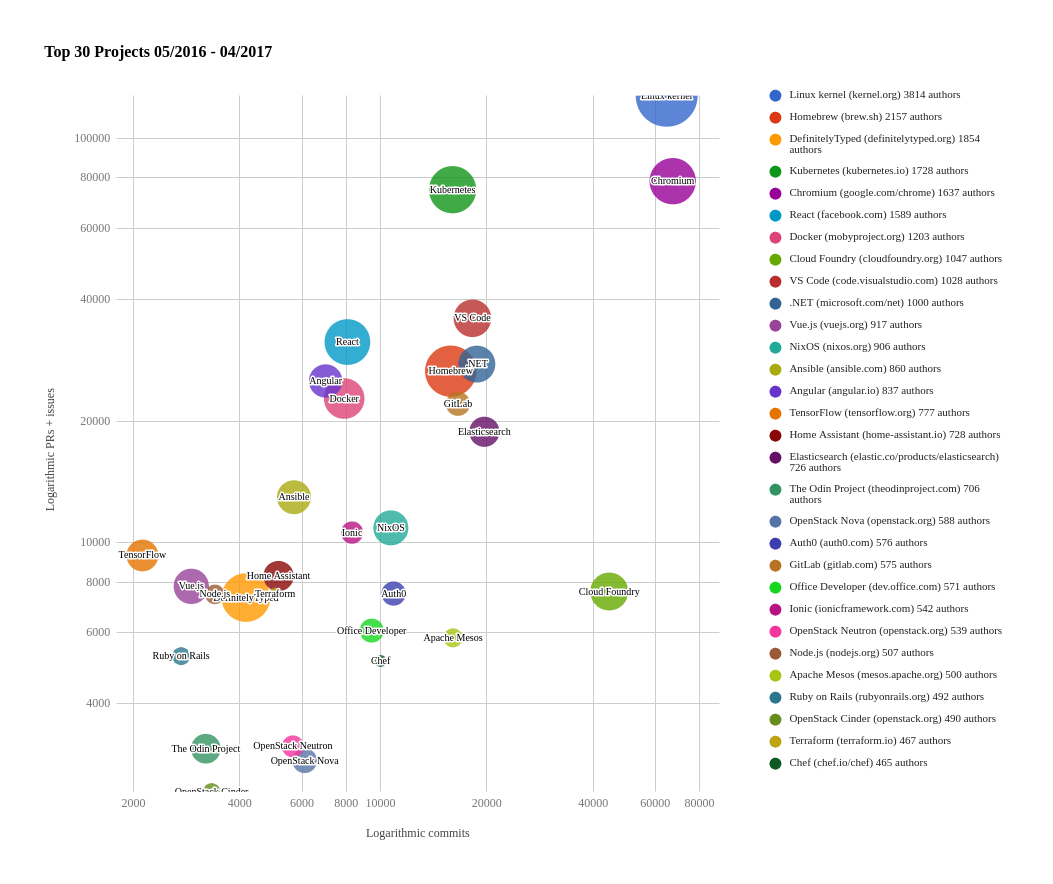
\includegraphics{images/project-velocity_visualization.png}

\href{https://www.cncf.io/blog/2017/06/05/30-highest-velocity-open-source-projects/}{From
CNCF}

\hypertarget{tools-providing-the-metric}{%
\subparagraph{Tools providing the
Metric}\label{tools-providing-the-metric}}

\begin{itemize}
\tightlist
\item
  CNCF -
  \href{https://github.com/cncf/velocity}{https://github.com/cncf/velocity}
\end{itemize}

\hypertarget{references}{%
\paragraph{References}\label{references}}

\begin{itemize}
\tightlist
\item
  \href{https://www.threefivetwo.com/blog/can-open-source-innovation-work-in-the-enterprise}{Can
  Open Source Innovation work in the Enterprise?}
\item
  \href{https://www.nearform.com/blog/want-a-high-performing-culture-make-way-for-open-innovation}{Open
  Innovation for a High Performance Culture}
\item
  \href{https://www.cio.com/article/3213146/open-source-is-powering-the-digital-enterprise.html}{Open
  Source for the Digital Enterprise}
\item
  \href{https://www.cncf.io/blog/2017/06/05/30-highest-velocity-open-source-projects}{Highest
  Velocity Open Source Projects}
\end{itemize}
 
 

\subsection{Focus Area - Individual-Value}
\textbf{Goal:} Identify if a project is valuable to me as an individual user or contributor.
\begin{table}[ht!]
    \centering
    \begin{tabular}{|p{0.35\linewidth} | p{0.6\linewidth}|}
        \hline
        \hfil \textbf{Metric}  & \hfil \textbf{Question} \\
        \hline
		Job Opportunities & How many job postings request skills with technologies from a project? \\ 
		\hline
		Organizational Project Skill Demand & How many organizations are using this project and could hire me if I become proficient? \\ 
		\hline
    \end{tabular}
\end{table}

\hypertarget{job-opportunities}{%
\section{Job Opportunities}\label{job-opportunities}}

Question: How many job postings request skills with technologies from a
project?

\hypertarget{description}{%
\subsection{Description}\label{description}}

A common way for open source contributors to earn a living wage is to be
employed by a company or be a self-employed or freelance developer.
Skills in a specific project may improve a job applicant's prospects of
getting a job. The most obvious indicator for demand related to a skill
learned in a specific open source project is when that project or its
technology is included in job postings.

\hypertarget{objectives}{%
\subsection{Objectives}\label{objectives}}

The metric gives contributors a sense of how much skills learned in a
specific open source project are valued by companies.

\hypertarget{implementation}{%
\subsection{Implementation}\label{implementation}}

To obtain this metric on a job search platform (e.g., LinkedIn, Indeed,
or Dice), go to the job search and type in the name of the open source
project. The number of returned job postings is the metric. Periodically
collecting the metric through an API of a job search platform and
storing the results allows to see trends.

\hypertarget{filters}{%
\subsubsection{Filters}\label{filters}}

\begin{itemize}
\tightlist
\item
  Age of job posting; postings get stale and may not be removed when
  filled
\end{itemize}

\hypertarget{visualizations}{%
\subsubsection{Visualizations}\label{visualizations}}

The metric can be extended by looking at:

\begin{itemize}
\tightlist
\item
  Salary ranges for jobs returned
\item
  Level of seniority for jobs returned
\item
  Availability of jobs like on-site or off-site
\item
  Location of job
\item
  Geography
\end{itemize}

\hypertarget{references}{%
\subsection{References}\label{references}}

\begin{itemize}
\tightlist
\item
  LinkedIn Job Search API:
  \url{https://developer.linkedin.com/docs/v1/jobs/job-search-api\#}
\item
  Indeed Job Search API:
  \url{https://opensource.indeedeng.io/api-documentation/docs/job-search/}
\item
  Dice.com Job Search API:
  \url{http://www.dice.com/external/content/documentation/api.html}
\item
  Monster Job Search API: \url{https://partner.monster.com/job-search}
\item
  Ziprecruiter API (Requires Partnership):
  \url{https://www.ziprecruiter.com/zipsearch}
\end{itemize}

\emph{Note:} This metric is limited to individual projects but
engagement in open source can be beneficial for other reasons. This
metric could be tweaked to look beyond a single project and instead use
related skills such as programming languages, processes, open source
experience, or frameworks as search parameters for jobs.
 
\hypertarget{organizational-project-skill-demand}{%
\section{Organizational Project Skill
Demand}\label{organizational-project-skill-demand}}

Question: How many organizations are using this project and could hire
me if I become proficient?

\hypertarget{description}{%
\subsection{Description}\label{description}}

Organizations engage with open source projects through use and
dependencies. This metric is aimed at determining downstream demand of
skills related to an open source project. This metric looks at
organizations that deploy a project as part of an IT infrastructure,
other open source projects with declared dependencies, and references to
the project through social media, conference mentions, blog posts, and
similar activities.

\hypertarget{objectives}{%
\subsection{Objectives}\label{objectives}}

As a developer, I'd like to invest my skills and time in a project that
has a likelihood of getting me a decent paying job in the future. People
can use the Downstream Organizational Impact of a Project Software
metric to discover which projects are used by organizations, and they
may, therefore, be able to pursue job opportunities with, possibly
requiring IT support services.

\hypertarget{implementation}{%
\subsection{Implementation}\label{implementation}}

Base metrics include:

\begin{itemize}
\tightlist
\item
  Number of organizations that created issues for a project
\item
  Number of organizations that created pull requests for a project
\item
  Number of organizations that blog or tweet about a project
\item
  Number of organizations that mention a project in open hiring requests
\item
  Number of organizations that are represented at meetups about this
  project
\item
  Number of other projects that are dependent on a project
\item
  Number of books about a project
\item
  Google search trends for a project
\end{itemize}

\hypertarget{visualizations}{%
\subsubsection{Visualizations}\label{visualizations}}

The following visualization demonstrates the number of downstream
projects dependendent on the project in question. While this
visualization does not capture the entirety of the Downstream
Organizational Impact of a Project Software metric, it provides a visual
for a portion.

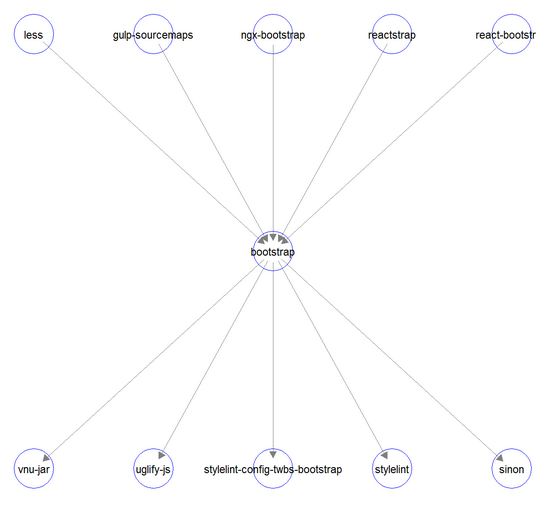
\includegraphics{images/organizational-project-skill-demand_paper.png}

Other visualizations could include Google search trends (React vs.
Angular vs. Vue.js)

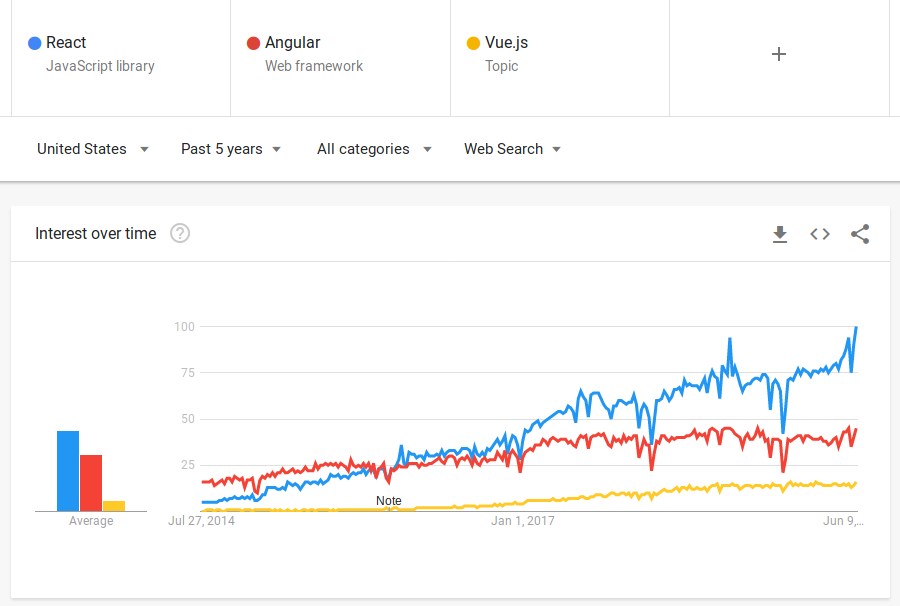
\includegraphics{images/organizational-project-skill-demand_google-trends.png}

ThoughtWorks publishes a series called 'Tech Radar' that shows the
popularity of technologies.

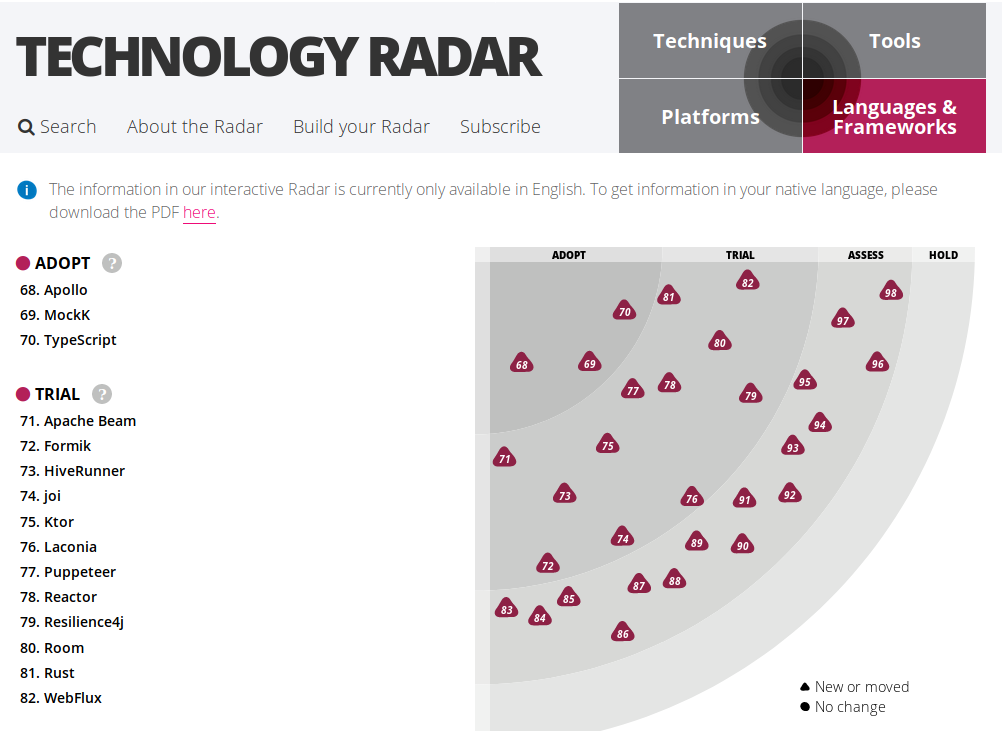
\includegraphics{images/organizational-project-skill-demand_tech-radar.png}

Tech Radar allows you to drill down on projects to see how the
assessment has changed over time.

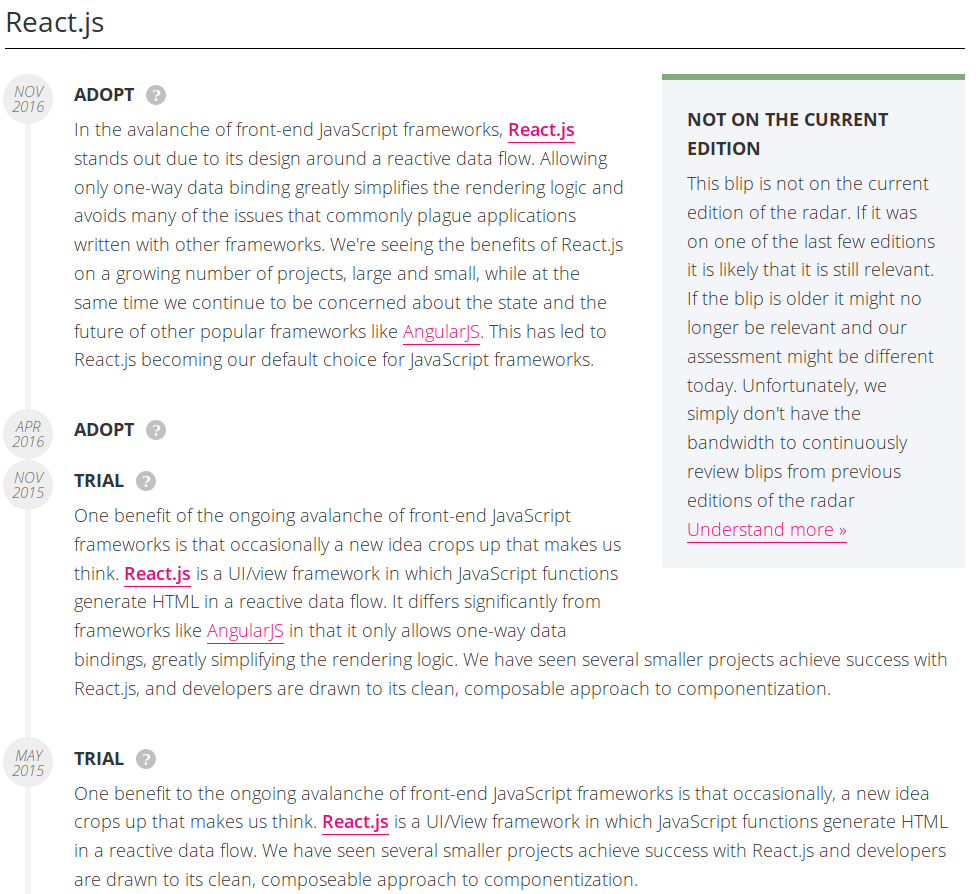
\includegraphics{images/organizational-project-skill-demand_tech-react.png}

StackOverview publishes an annual developer's survey

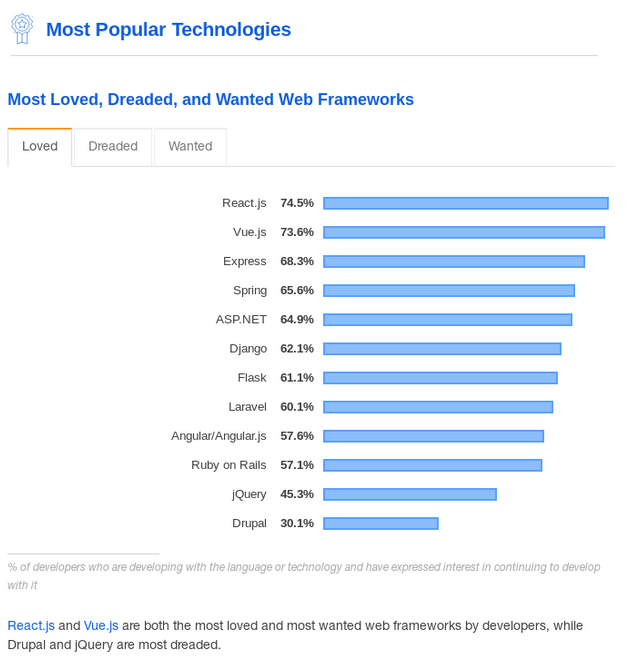
\includegraphics{images/organizational-project-skill-demand_stack-overflow.png}

\hypertarget{tools-providing-the-metric}{%
\subsubsection{Tools Providing the
Metric}\label{tools-providing-the-metric}}

\begin{itemize}
\tightlist
\item
  Google Trends - for showing search interest over time
\item
  ThoughtWorks TechRadar - project assessments from a tech consultancy
\item
  StackOverflow Developer's Survey - annual project rankings
\item
  Augur; Examples are available for multiple repositories:

  \begin{itemize}
  \tightlist
  \item
    \href{http://augur.osshealth.io/repo/Rails\%20(wg-value)/rails/overview}{Rails}
  \item
    \href{http://augur.osshealth.io/repo/Zephyr-RTOS/zephyr/overview}{Zephyr}
  \item
    \href{http://augur.osshealth.io/repo/Apache\%20(wg-value)/cloudstack/overview}{CloudStack}
  \end{itemize}
\end{itemize}

\hypertarget{references}{%
\subsection{References}\label{references}}

\begin{itemize}
\tightlist
\item
  \href{https://opensource.org/sponsors}{Open Source Sponsors}
\item
  \href{https://opensource.com/article/19/1/fiscal-sponsors-open-source}{Fiscal
  Sponsors and Open Source}
\item
  \href{https://www.networkworld.com/article/2867020/big-names-like-google-dominate-open-source-funding.html}{Large
  Corporate OpenSource Sponsors}
\item
  \href{https://www.npmjs.com/package/google-trends-api}{Google Trends
  API}
\item
  \href{https://aisel.aisnet.org/cgi/viewcontent.cgi?article=1496\&context=amcis2018}{Measuring
  Open Source Software Impact}
\item
  \href{https://www.thoughtworks.com/radar}{ThoughtWorks Tech Radar}
\item
  \href{https://insights.stackoverflow.com/survey/2019\#technology}{Stack
  Overflow Developer's Survey}
\end{itemize}
 
 

\subsection{Focus Area - Organizational Value}
\textbf{Goal:} Identify if a project is monetarily valuable from an organization's perspective.
\begin{table}[ht!]
    \centering
    \begin{tabular}{|p{0.35\linewidth} | p{0.6\linewidth}|}
        \hline
        \hfil \textbf{Metric}  & \hfil \textbf{Question} \\
        \hline
    		Labor Investment & What was the cost of an organization for its employees to create the counted contributions (e.g., commits, issues, and pull requests)? \\ 
		\hline
    \end{tabular}
\end{table}
    
\hypertarget{ux4ebaux529bux6295ux8d44}{%
\subsubsection{人力投资}\label{ux4ebaux529bux6295ux8d44}}

问题:组织投入人力对社区所做的贡献(例如:代码提交,议题和更改请求)花费的成本是多少

\hypertarget{ux63cfux8ff0}{%
\paragraph{描述}\label{ux63cfux8ff0}}

开源项目通常由组织的人力投入来支撑。该指标跟踪组织对单个项目的经济投入(体现在人力成本)。

\hypertarget{ux76eeux6807}{%
\paragraph{目标}\label{ux76eeux6807}}

随着组织参与度对开源项目变得越来越重要,组织必须清楚了解其人力投资。该指标的目的是为从事开源项目的组织提高人力成本的透明度。该指标给开源项目办公室(OSPO)经理提供了一种通过项目投资组合比较人力成本的方法。比如:人力投资指标能用在确定投资的优先顺序或者确定投资回报。例如:

\begin{itemize}
\tightlist
\item
  以人力投资评估 OSPO 事务的优先级和证明预算合理性
\item
  以人力投资解释产品、项目管理事项的优先级
\item
  以人力投资论证继续投资 OSPO 的价值
\item
  以人力投资反应和比较开源贡献与内部工作的人力成本
\item
  以人力投资比较项目组合的项目效益
\end{itemize}

\hypertarget{ux5b9eux73b0}{%
\paragraph{实现}\label{ux5b9eux73b0}}

基础指标包括:

\begin{itemize}
\tightlist
\item
  贡献数量
\item
  按贡献者类型(内部/外部)划分的贡献数量
\item
  按贡献类型(如代码提交,议题和更改请求)划分的贡献数量
\end{itemize}

参数包括:

\begin{itemize}
\tightlist
\item
  每小时劳动率
\item
  创建贡献的平均劳动时间(按照贡献类型分类)
\end{itemize}

人力投资 = 每一种贡献类型的总和(贡献数量 * 创造贡献的平均工时 *
平均每小时劳动率)

\hypertarget{ux7b5bux9009ux6761ux4ef6}{%
\subparagraph{筛选条件}\label{ux7b5bux9009ux6761ux4ef6}}

\begin{itemize}
\tightlist
\item
  内部与外部贡献者
\item
  问题标签
\item
  项目来源(如内部、开源仓库、竞争对手的开源仓库)
\end{itemize}

\hypertarget{ux53efux89c6ux5316ux6548ux679c}{%
\subparagraph{可视化效果}\label{ux53efux89c6ux5316ux6548ux679c}}

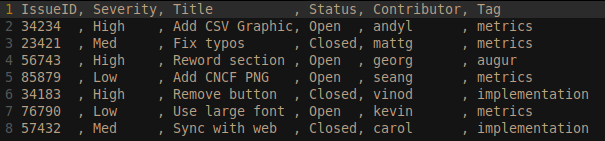
\includegraphics{images/labor-investment_csv.png}

我们的第一个参数化指标的可视化效果依赖于可以用Augur导出的CSV。电子表格用于指标参数和计算公式。未来的实现可能会在
webapp 中直接添加参数操作的功能。

\hypertarget{ux53c2ux8003ux8d44ux6599}{%
\paragraph{参考资料}\label{ux53c2ux8003ux8d44ux6599}}

\begin{itemize}
\tightlist
\item
  \href{https://www.slideshare.net/caniszczyk/starting-an-open-source-program-office-ospo}{启动开源项目办公室}
\item
  \href{https://events19.linuxfoundation.org/wp-content/uploads/2018/07/OSLS_2019-untold-story-of-OSPO.pdf}{创办开源项目办公室}
\item
  \href{https://d1.awsstatic.com/Open\%20Source/enterprise-oss-book.pdf}{企业开源}
\end{itemize}
 
 
 

\end{document}

\section{Common Metrics WG}
\clearpage

\hypertarget{technical-fork}{%
\subsubsection{Technical Fork}\label{technical-fork}}

Question: What are a number of technical forks of an open source project
on code development platforms?

\hypertarget{description}{%
\paragraph{Description}\label{description}}

A technical fork is a distributed version control copy of a project. The
number of technical forks indicates the number of copies of a project on
the same code development platform.

\hypertarget{objectives}{%
\paragraph{Objectives}\label{objectives}}

The objective of the Technical Fork metric is to ascertain how many
copies of a project exist on a code development platform. Analysis of
technical forks may provide insight into forking intentions (different
types of forks such as contributing, and non-contributing forks).

\hypertarget{implementation}{%
\paragraph{Implementation}\label{implementation}}

\hypertarget{filters}{%
\subparagraph{Filters}\label{filters}}

\begin{itemize}
\tightlist
\item
  Time Period (e.g., Weekly, Monthly, Annually)
\item
  Ratio of contributing fork to total forks (A contributing fork is a
  fork that has opened a change request against the original
  repository.)
\item
  Ratio of non-contributing fork to total forks (A non-contributing fork
  is a fork that has never opened a change request against the original
  repository.)
\end{itemize}

\hypertarget{visualizations}{%
\subparagraph{Visualizations}\label{visualizations}}

\textbf{Augur Implementation}\\
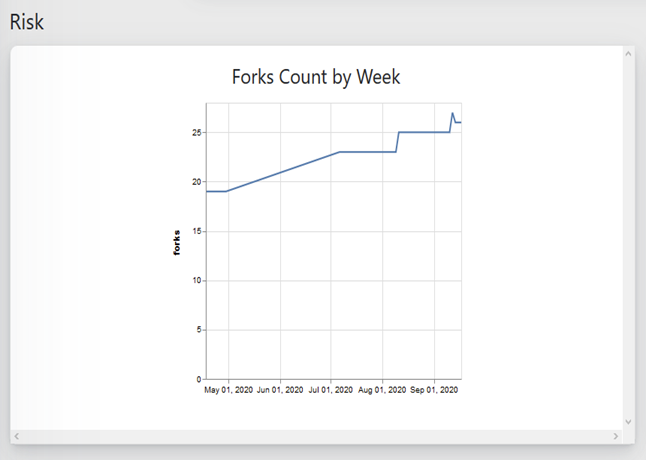
\includegraphics{images/technical-fork_augur-fork.png}

\textbf{GrimoireLab Implementation}\\
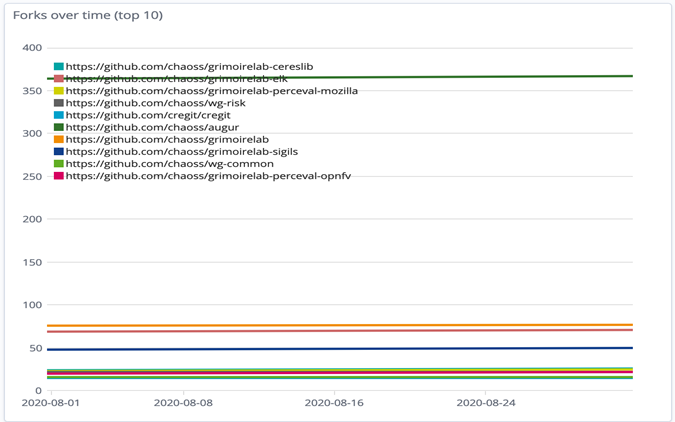
\includegraphics{images/technical-fork_grimoirelab-fork.png}

\hypertarget{tools-providing-the-metric}{%
\subparagraph{Tools Providing the
Metric}\label{tools-providing-the-metric}}

\begin{itemize}
\tightlist
\item
  Augur
\item
  GrimoireLab
\end{itemize}

\hypertarget{data-collection-strategies}{%
\subparagraph{Data Collection
Strategies}\label{data-collection-strategies}}

\textbf{Github API}\\
\url{https://developer.github.com/v3/repos/forks/\#list-forks}

\textbf{GitLab API}\\
\url{https://docs.gitlab.com/ee/api/projects.html\#list-forks-of-a-project}

\textbf{Bitbucket API}\\
\url{https://developer.atlassian.com/bitbucket/api/2/reference/resource/repositories/\%7Bworkspace\%7D/\%7Brepo_slug\%7D/forks}

\hypertarget{references}{%
\paragraph{References}\label{references}}

\url{https://help.github.com/en/enterprise/2.13/user/articles/fork-a-repo}
\url{https://opensource.com/article/17/12/fork-clone-difference}
 
\hypertarget{ux8d21ux732eux7c7bux578b}{%
\subsubsection{贡献类型}\label{ux8d21ux732eux7c7bux578b}}

问题:正在进行哪些类型的贡献?

\hypertarget{ux63cfux8ff0}{%
\paragraph{描述}\label{ux63cfux8ff0}}

多元化的贡献能够使开源项目健康发展。在很多项目中,有些社区成员并不编写代码,但他们同样做出了有价值的贡献,比如管理社区、区分错误、宣传项目、支持用户或以其他方式提供帮助。

\hypertarget{ux76eeux6807}{%
\paragraph{目标}\label{ux76eeux6807}}

多样的贡献类型表明项目是成熟全面的,包含足够的活动来支持项目的所有方面,并且提供多种贡献类型的晋升渠道,让拥有编码之外的不同专长的人员也能够发展到领导层。

\hypertarget{ux5b9eux73b0}{%
\paragraph{实现}\label{ux5b9eux73b0}}

如何对贡献进行定义、量化、跟踪和公布是一个具有挑战性的问题。
每个项目的答案可能都是独一无二的,以下建议仅作为抛砖引玉。作为一个通用指南,很难将不同的贡献类型相互比较,应单独考量。

\begin{itemize}
\tightlist
\item
  以下列表可以帮助确定贡献类型:

  \begin{itemize}
  \tightlist
  \item
    编写代码
  \item
    审查代码
  \item
    错误分类
  \item
    质量保证和测试
  \item
    安全相关活动
  \item
    本地化和翻译
  \item
    事件组织
  \item
    文档编写
  \item
    社区建设和管理
  \item
    教学和教程构建
  \item
    故障排除和支持
  \item
    创意作品和设计
  \item
    用户界面、用户体验和易用性
  \item
    社交媒体管理
  \item
    用户支持和问题解答
  \item
    撰写文章
  \item
    公共关系 - 技术媒体采访
  \item
    事件发言
  \item
    营销与活动宣传
  \item
    网站开发
  \item
    法律委员会
  \item
    财务管理
  \end{itemize}
\end{itemize}

\hypertarget{ux6570ux636eux6536ux96c6ux7b56ux7565}{%
\subparagraph{数据收集策略}\label{ux6570ux636eux6536ux96c6ux7b56ux7565}}

\begin{itemize}
\item
  **采访或调查:**让社区成员认可他人的贡献,找出过去没有考虑到的贡献类型。

  \begin{itemize}
  \tightlist
  \item
    您想表彰谁在项目中的贡献? 他们贡献了什么?
  \end{itemize}
\item
  **观察项目:**找出和认可项目不同部分的负责人。

  \begin{itemize}
  \tightlist
  \item
    在项目网站或代码仓库中列出了哪些负责人?
  \end{itemize}
\item
  **捕获非代码贡献:**通过问题跟踪器等专用系统跟踪贡献。

  \begin{itemize}
  \tightlist
  \item
    日志记录可以包含项目要了解的关于非代码贡献的定制化信息,用以识别工作量。
  \item
    通过沟通渠道活动的代理贡献。 例如,如果质量保证成员 (QA)
    拥有自己的邮件列表,就可以通过邮件列表活动来代理衡量围绕 QA
    贡献的活动。
  \end{itemize}
\item
  **收集跟踪数据:**通过协作工具日志数据衡量贡献。

  \begin{itemize}
  \tightlist
  \item
    例如,可以从源代码仓库计算代码贡献,可以从维基编辑历史记录计算维基贡献,可以从电子邮件归档计算电子邮件消息
  \end{itemize}
\item
  **自动分类:**训练人工智能 (AI) 机器人来检测贡献并对其分类。

  \begin{itemize}
  \tightlist
  \item
    AI
    机器人可以协助对贡献进行分类,例如,帮助请求与提供的支持,或功能请求与错误报告,尤其是以上均在同一个问题跟踪器中完成的情况。
  \end{itemize}
\end{itemize}

\emph{其他考量:}

\begin{itemize}
\tightlist
\item
  特别是对于自动报告,允许社区成员选择退出并不出现在贡献报告上。
\item
  承认对贡献类型的捕捉不完善,并明确说明收集了哪些类型的贡献。
\item
  随着项目发展,贡献类型的收集方法需要作出调整。
  例如,交换国际化库时,围绕本地化的项目活动可能会在变化前后产生不同的指标。
\item
  大规模挖掘贡献类型时,要考虑机器人的活动。
\end{itemize}

\hypertarget{ux53c2ux8003ux8d44ux6599}{%
\paragraph{参考资料}\label{ux53c2ux8003ux8d44ux6599}}

\begin{itemize}
\tightlist
\item
  \href{https://medium.com/@sunnydeveloper/revisiting-the-word-recognition-in-foss-and-the-dream-of-open-credentials-d15385d49447}{https://medium.com/@sunnydeveloper/revisiting-the-word-recognition-in-foss-and-the-dream-of-open-credentials-d15385d49447}
\item
  \href{https://24pullrequests.com/contributing}{https://24pullrequests.com/contributing}
\item
  \href{https://smartbear.com/blog/test-and-monitor/14-ways-to-contribute-to-open-source-without-being/}{https://smartbear.com/blog/test-and-monitor/14-ways-to-contribute-to-open-source-without-being/}
\item
  \href{https://wiki.openstack.org/wiki/AUCRecognition}{https://wiki.openstack.org/wiki/AUCRecognition}
\item
  \href{https://www.drupal.org/drupalorg/blog/a-guide-to-issue-credits-and-the-drupal.org-marketplace}{https://www.drupal.org/drupalorg/blog/a-guide-to-issue-credits-and-the-drupal.org-marketplace}
\end{itemize}
 
 

\subsection{Focus Area - When}
\textbf{Goal:} Understand when contributions from organizations and people are happening.
\begin{table}[ht!]
    \centering
    \begin{tabular}{|p{0.35\linewidth} | p{0.6\linewidth}|}
        \hline
        \hfil \textbf{Metric}  & \hfil \textbf{Question} \\
        \hline
		Activity Dates and Times & What are the dates and timestamps of when contributor activities occur? \\ 
		\hline
		Burstiness & How are short timeframes of intense activity, followed by a corresponding return to a typical pattern of activity, observed in a project? \\ 
		\hline
		Review Cycle Duration within a Change Request & What is the duration of a review cycle within a single change request? \\ 
		\hline
		Time to Close & How much time passes between creating and closing an operation such as an issue, change request, or support ticket? \\ 
		\hline
		Time to First Response & How much time passes between when an activity requiring attention is created and the first response? \\ 
		\hline
    \end{tabular}
\end{table}

\hypertarget{activity-dates-and-times}{%
\section{Activity Dates and Times}\label{activity-dates-and-times}}

Question: What are the dates and timestamps of when contributor
activities occur?

\hypertarget{description}{%
\subsection{Description}\label{description}}

Individuals engage in activities in open source projects at various
times of the day. This metric is aimed at determining the dates and
times of when individual activities were completed. The data can be used
to probabilistically estimate where on earth contributions come from in
cases where the time zone is not UTC.

\hypertarget{objectives}{%
\subsection{Objectives}\label{objectives}}

\begin{itemize}
\tightlist
\item
  Improve transparency for employers about when organizational employees
  are engaging with open source projects
\item
  Improve transparency for open source project and community managers as
  to when activity is occurring
\end{itemize}

\hypertarget{implementation}{%
\subsection{Implementation}\label{implementation}}

\hypertarget{filters}{%
\subsubsection{Filters}\label{filters}}

\begin{itemize}
\tightlist
\item
  Individual by Organization
\item
  Aggregation of time by UTC time

  \begin{itemize}
  \tightlist
  \item
    Can show what times across the globe contributions are made; when
    the project is most active.
  \end{itemize}
\item
  Aggregation of time by local time

  \begin{itemize}
  \tightlist
  \item
    Can show what times of day in their local times they contribute.
    Conclusions about the If contributions are more during working
    hours, or if contributions are more during evening hours.
  \end{itemize}
\item
  Repository ID
\item
  Segment of a community, (e.g., GrimoireLab has more EU time zones
  activity and Augur more US time zones activity)
\end{itemize}

\hypertarget{visualizations}{%
\subsubsection{Visualizations}\label{visualizations}}

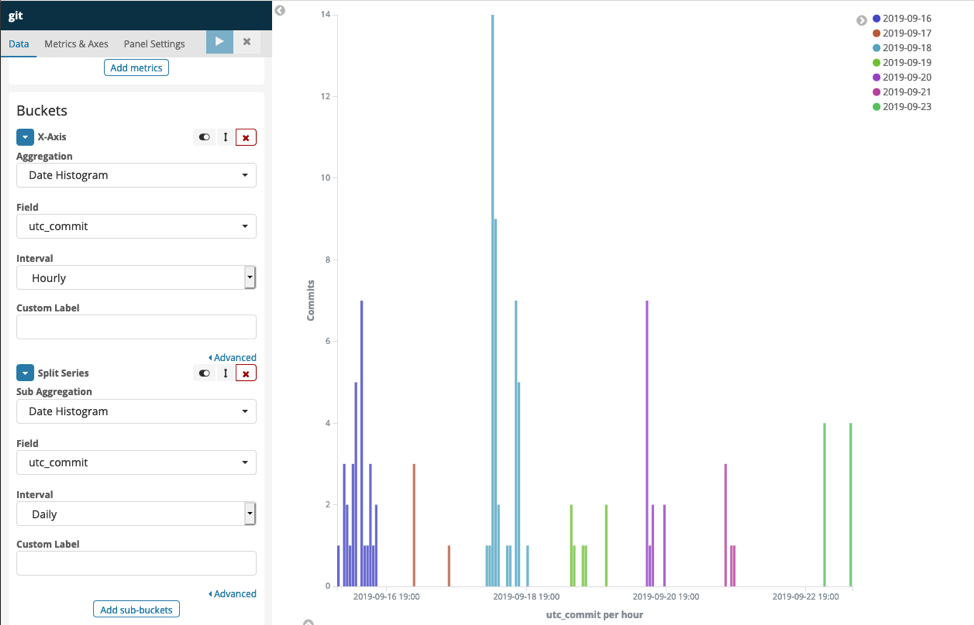
\includegraphics{images/activity-dates-and-times_1.png}
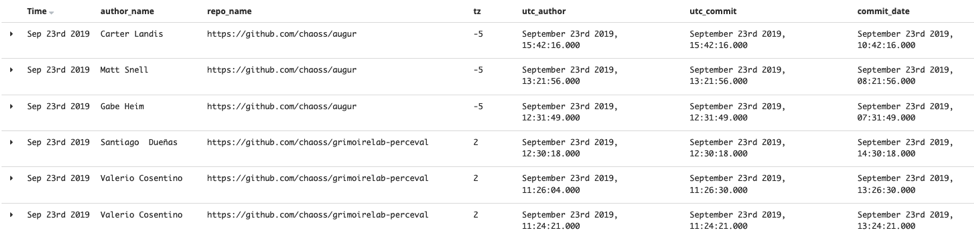
\includegraphics{images/activity-dates-and-times_2.png}
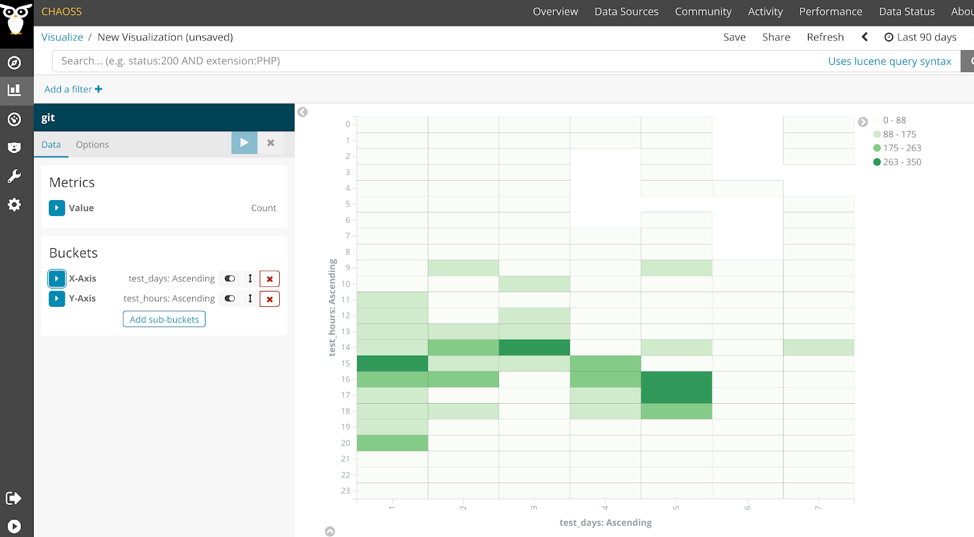
\includegraphics{images/activity-dates-and-times_3.png}
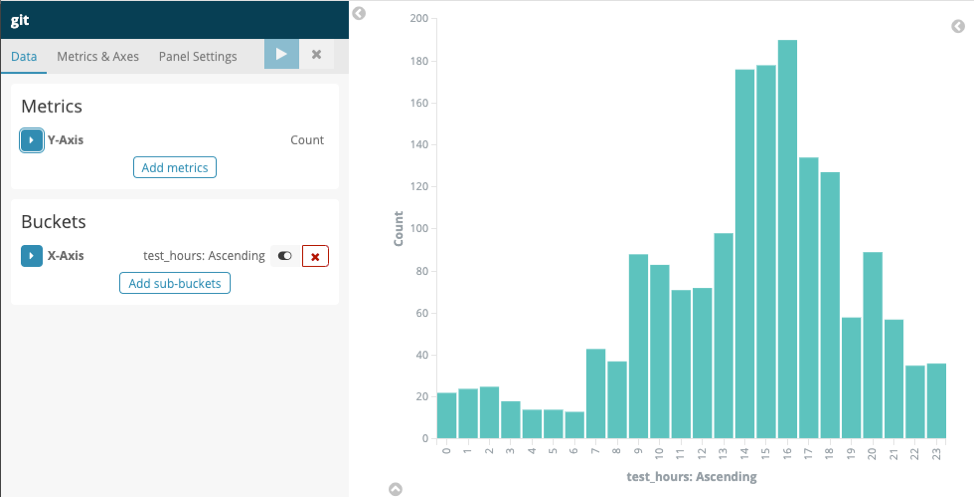
\includegraphics{images/activity-dates-and-times_4.png}

\hypertarget{tools-providing-metric}{%
\subsubsection{Tools Providing Metric}\label{tools-providing-metric}}

\href{https://chaoss.github.io/grimoirelab/}{GrimoireLab}

\href{https://docs.augur.net/\#dates-timestamps}{Augur Date/Timestamps}

\hypertarget{references}{%
\subsection{References}\label{references}}

\href{https://en.wikipedia.org/wiki/Coordinated_Universal_Time}{Coordinated
Universal Time}
 
\hypertarget{burstiness}{%
\section{Burstiness}\label{burstiness}}

Question: How are short timeframes of intense activity, followed by a
corresponding return to a typical pattern of activity, observed in a
project?

\hypertarget{description}{%
\subsection{Description}\label{description}}

There are a number of reasons that may prompt a sudden increase or
decrease in the amount of activity within a repository. These increases
and decreases appear both as a sudden change in activity against the
average amount of activity. Burstiness is a way of understanding the
cycle of activity in existing metrics, like issues, merge requests,
mailing lists, commits, or comments. Examples of root causes for bursts
in activity include:

\begin{itemize}
\tightlist
\item
  Release cycles
\item
  Global pandemics
\item
  Hackathon activities
\item
  Mentorship programs
\item
  Conferences, meetups, and other events where tools are presented
\item
  Conventional and social media announcements and mentions
\item
  Critical bugs as raising awareness and getting people's attention
\item
  Community design meetings or brainstorming meetings to address a
  particular issue
\item
  Community members show up from another community that is relying on
  your project (e.g., dependencies)
\end{itemize}

\hypertarget{objectives}{%
\subsection{Objectives}\label{objectives}}

\begin{itemize}
\tightlist
\item
  To identify impacts of root causes of a burst in activity
\item
  To provide awareness when project activity unknowingly goes up
\item
  To help capture the meaningfulness of increases or decreases in
  project activity
\item
  To help the community and maintainers prepare for future bursts that
  follow a pattern
\item
  To help measure the impact of influential external activities
\item
  To differentiate skewed activity versus normal activity
\end{itemize}

\hypertarget{implementation}{%
\subsection{Implementation}\label{implementation}}

\hypertarget{filters}{%
\subsubsection{Filters}\label{filters}}

\begin{itemize}
\tightlist
\item
  Stars
\item
  Forks
\item
  Issues or bug reports
\item
  Labels
\item
  Downloads
\item
  Release Tags
\item
  Change Requests
\item
  Mail List Traffic
\item
  Documentation additions or revisions
\item
  New Repositories
\item
  Feature Requests
\item
  Messaging Conversations
\item
  Conventional and Social Media Activity
\item
  Conference Attendance and Submissions
\end{itemize}

\hypertarget{visualizations}{%
\subsubsection{Visualizations}\label{visualizations}}

Augur:

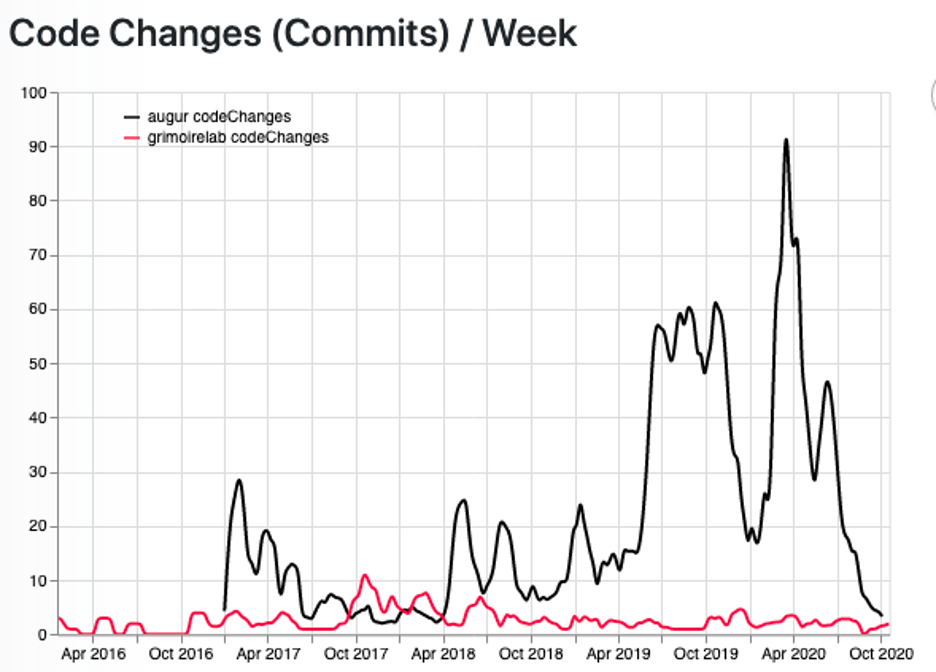
\includegraphics{images/burstiness_augur.png}

GrimoireLab:

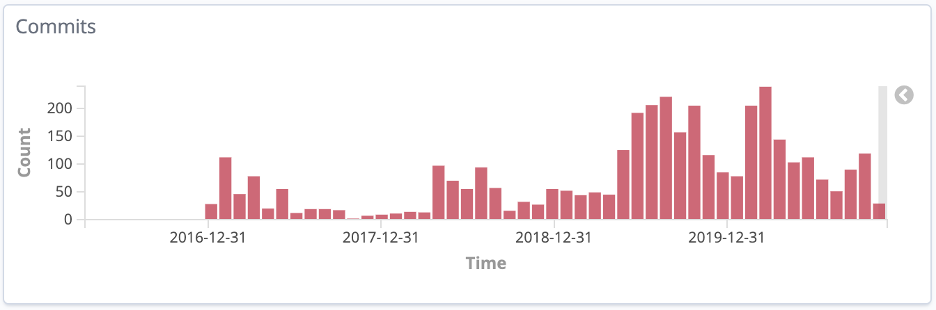
\includegraphics{images/burstiness_gl.png}

\hypertarget{tools-providing-the-metric}{%
\subsubsection{Tools Providing the
Metric}\label{tools-providing-the-metric}}

\begin{itemize}
\tightlist
\item
  Grimoire Lab
\item
  Augur
\end{itemize}

\hypertarget{data-collection-strategies}{%
\subsubsection{Data Collection
Strategies}\label{data-collection-strategies}}

\begin{itemize}
\item
  Quantitative

  \begin{itemize}
  \tightlist
  \item
    Time box activities identifying deviations away from some norm
  \item
    Outliers for certain thresholds, using statistics like Bollinger
    Bands to measure stability or volatility:
    \url{https://en.wikipedia.org/wiki/Bollinger_Bands}
  \end{itemize}
\item
  Qualitative Interview Questions

  \begin{itemize}
  \tightlist
  \item
    Why do you contribute more during a period of time?
  \item
    What do you believe to be the root cause for particular bursts?
  \item
    What impact do different events (e.g., hackathons, mentorship
    program, or conferences) have on project activity?
  \end{itemize}
\end{itemize}

\hypertarget{references}{%
\subsection{References}\label{references}}

This metric was inspired by the work of Goh and Barabasi (2008):
\url{https://arxiv.org/pdf/physics/0610233.pdf}
 
\hypertarget{review-cycle-duration-within-a-change-request}{%
\subsubsection{Review Cycle Duration within a Change
Request}\label{review-cycle-duration-within-a-change-request}}

Question: What is the duration of a review cycle within a single change
request?

\hypertarget{description}{%
\paragraph{Description}\label{description}}

A change request is based on one or more review cycles. Within a review
cycle, one or more reviewers can provide feedback on a proposed
contribution. The duration of a review cycle, or the time between each
new iteration of the contribution, is the basis of this metric.

\hypertarget{objectives}{%
\paragraph{Objectives}\label{objectives}}

This metric provides maintainers with insight on: Code review process
decay, as there are more iterations and review cycle durations increase.
Process bottlenecks resulting in long code review iterations. Abandoned
or semi-abandoned processes in the review cycles, where either the
maintainer or the submitter is slow in responding. Characteristics of
reviews that have different cyclic pattern lengths.

\hypertarget{implementation}{%
\paragraph{Implementation}\label{implementation}}

Review Cycle Duration is measured as the time length of one review cycle
within a single change request. The duration can be calculated between:
The moment when each review cycle begins, defined as the point in time
when a change request is submitted or updated. The moment when each
review cycle ends, either because the change request was updated and
needs a new review or because it was accepted or rejected.

\hypertarget{filter}{%
\subparagraph{Filter}\label{filter}}

Average or Median Duration, optionally filtered or grouped by: Number of
people involved in review Number of comments in review Edits made to a
change request Project or program Organization making the change request
Time the change request was submitted Developers who contributed to a
change request Change request Number of review cycle on a change request
(e.g., filter by first, second, \ldots{} round)

\hypertarget{visualizations}{%
\subparagraph{Visualizations}\label{visualizations}}

\hypertarget{tools-providing-the-metric}{%
\subparagraph{Tools Providing the
Metric}\label{tools-providing-the-metric}}

\hypertarget{references}{%
\paragraph{References}\label{references}}

Example of data that could be used to develop the metric:
\url{https://gerrit.wikimedia.org/r/c/mediawiki/core/+/194071}
 
\hypertarget{ux5173ux95edux65f6ux957f}{%
\subsubsection{关闭时长}\label{ux5173ux95edux65f6ux957f}}

问题:创建和关闭操作(如议题、更改请求或需要支持的问题单)之间需要多少时间?

\hypertarget{ux63cfux8ff0}{%
\paragraph{描述}\label{ux63cfux8ff0}}

关闭时长是指从创建到关闭操作(如议题、更改请求或需要支持的问题单)的总时长。
操作需要具有打开和关闭的状态,比如代码审查进程、问答论坛、问题跟踪系统中经常出现的情况。

相关指标:\href{https://chaoss.community/metric-issue-resolution-duration/}{问题解决时长}

\hypertarget{ux76eeux6807}{%
\paragraph{目标}\label{ux76eeux6807}}

\begin{enumerate}
\def\labelenumi{\arabic{enumi}.}
\tightlist
\item
  确定社区的响应程度,帮助增加包容性,吸引新贡献者并保留现有贡献者。
\item
  找出导致快速或缓慢关闭的操作特征(如寻找最佳实践、改进领域、评估效率)。
\item
  识别对不同社区成员及时响应的偏差。
\item
  检测社区活动的变化(例如,显示潜在的维护者倦怠、贡献多元化的减少)
\item
  了解关闭议题或更改请求的时间与合并成功或失败的关系
\end{enumerate}

\hypertarget{ux5b9eux73b0}{%
\paragraph{实现}\label{ux5b9eux73b0}}

\hypertarget{ux7b5bux9009ux6761ux4ef6}{%
\subparagraph{筛选条件}\label{ux7b5bux9009ux6761ux4ef6}}

\begin{itemize}
\tightlist
\item
  操作的创建者(例如,新贡献者相对于维护者)
\item
  最初关闭,最后关闭
\item
  标签(例如错误与新功能)
\item
  更改请求合并状态(例如,合并时间或没有合并的关闭时间)
\end{itemize}

\hypertarget{ux53efux89c6ux5316ux6548ux679c}{%
\subparagraph{可视化效果}\label{ux53efux89c6ux5316ux6548ux679c}}

\includegraphics{images/time-to-close_1.png}

\hypertarget{ux63d0ux4f9bux6307ux6807ux7684ux5de5ux5177}{%
\subparagraph{提供指标的工具}\label{ux63d0ux4f9bux6307ux6807ux7684ux5de5ux5177}}

Augur 实现:

\begin{itemize}
\tightlist
\item
  \href{http://augur.osshealth.io/api_docs/\#api-Evolution-Closed_Issue_Resolution_Duration(Repo)}{问题解决时长}
\item
  \href{http://augur.osshealth.io/api_docs/\#api-Evolution-issue-duration-repo}{问题持续时间}
\item
  \href{http://augur.osshealth.io/api_docs/\#api-Evolution-Issue_Response_Time(Repo)}{问题响应时间}
\end{itemize}

GrimoireLab 实现:

\begin{itemize}
\tightlist
\item
  \href{https://chaoss.github.io/grimoirelab-sigils/panels/github-pullrequests-efficiency/}{拉取请求效率}
\item
  \href{https://chaoss.github.io/grimoirelab-sigils/panels/github-issues-efficiency/}{问题效率}
\item
  \href{https://chaoss.github.io/grimoirelab-sigils/panels/efficiency-timing-overview/}{Efficiency:TimingOverview}
\end{itemize}

\hypertarget{ux6570ux636eux6536ux96c6ux7b56ux7565}{%
\subparagraph{数据收集策略}\label{ux6570ux636eux6536ux96c6ux7b56ux7565}}

关闭时长指标可根据项目活动和目标的具体情况而定。
例如,错误报告的关闭时长可能提供与新功能请求的关闭时长不同的信息。
数据收集策略应针对不同的项目目标。 可能影响这些进程的其他变量是:

\begin{itemize}
\tightlist
\item
  问题跟踪系统:如错误报告、蓝图 (OpenStack 专有命名)、用户故事(user
  story)、功能请求、epic等可能会影响事件关闭时长的议题类型。
  优先级或严重性等其他变量可能有助于推进这一事件的关闭速度。
\item
  变更请求流程:这取决于变更请求的平台架构,如 Gerrit、GitHub
  或邮件列表(如 Linux 内核中),并可能根据进程的复杂程度而有所不同。
  例如,新人和经验丰富的高级开发者将以不同的方式开展进程,所需时间或多或少。
\item
  问答论坛:这取决于回答的质量和提问者的意见。
  有效答案会被标记,提问者成功找到自己问题的正确答案后,进程随即关闭。
\end{itemize}

\hypertarget{ux53c2ux8003ux8d44ux6599}{%
\paragraph{参考资料}\label{ux53c2ux8003ux8d44ux6599}}

\begin{itemize}
\tightlist
\item
  ``Practice P.12: Respond to all submissions'',出自``Appendix to:
  Managing Episodic Volunteers in Free/Libre/Open Source Software
  Communities'',Ann Barcomb、Klaas-Jan Stol、Brian Fitzgerald 和 Dirk
  Riehle:\href{https://opus4.kobv.de/opus4-fau/frontdoor/index/index/docId/13519}{https://opus4.kobv.de/opus4-fau/frontdoor/index/index/docId/13519}
\end{itemize}
 
\hypertarget{time-to-first-response}{%
\subsubsection{Time to First Response}\label{time-to-first-response}}

Question: How much time passes between when an activity requiring
attention is created and the first response?

\hypertarget{description}{%
\paragraph{Description}\label{description}}

The first response to an activity can sometimes be the most important
response. The first response shows that a community is active and
engages in conversations. A long time to respond to an activity can be a
sign that a community is not responsive. A short time to respond to an
activity can help to engage more members into further discussions and
within the community.

\hypertarget{objectives}{%
\paragraph{Objectives}\label{objectives}}

Identify cadence of first response across a variety of activities,
including PRs, Issues, emails, IRC posts, etc. Time to first response is
an important consideration for new and long-time contributors to a
project along with overall project health.

\hypertarget{implementation}{%
\paragraph{Implementation}\label{implementation}}

Time to first response of an activity = time first response was posted
to the activity - time the activity was created.

\hypertarget{filters}{%
\subparagraph{Filters}\label{filters}}

\begin{itemize}
\tightlist
\item
  Role of responder, e.g., only count maintainer responses
\item
  Automated responses, e.g., only count replies from real people by
  filtering bots and other automated replies
\item
  Type of Activity, e.g., issues (see metric
  \href{https://github.com/chaoss/wg-evolution/blob/master/metrics/Issue_Response_Time.md}{Issue
  Response Time}), emails, chat, change requests
\end{itemize}

\hypertarget{visualizations}{%
\subparagraph{Visualizations}\label{visualizations}}

<<<<<<< HEAD
\includegraphics{images/time-to-first-response_efficiency-timing-overview.png}

\begin{center}\rule{0.5\linewidth}{0.5pt}\end{center}

\includegraphics{images/time-to-first-response_augur-ttc-1.png}

\begin{center}\rule{0.5\linewidth}{0.5pt}\end{center}
=======
\hypertarget{grimoirelab-panel-efficiency-timing-overview}{%
\subsection{\texorpdfstring{\protect\includegraphics{images/time-to-first-response_efficiency-timing-overview.png}}{GrimoireLab Panel: Efficiency Timing Overview}}\label{grimoirelab-panel-efficiency-timing-overview}}

\hypertarget{augur-visualization-time-to-first-response-heat-map-}{%
\subsection{\texorpdfstring{\protect\includegraphics{images/time-to-first-response_augur-ttc-1.png}}{Augur Visualization: Time to First Response Heat Map }}\label{augur-visualization-time-to-first-response-heat-map-}}
>>>>>>> main

\includegraphics{images/time-to-first-response_augur-ttc-2.png}

\hypertarget{tools-providing-the-metric}{%
\subparagraph{Tools Providing the
Metric}\label{tools-providing-the-metric}}

\begin{itemize}
\tightlist
\item
  GrimoireLab Panel:
  \href{https://chaoss.github.io/grimoirelab-sigils/panels/efficiency-timing-overview/}{Efficiency
  Timing Overview}
\item
  \href{https://katacontainers.biterg.io/app/kibana\#/dashboard/cbbdd920-288c-11e9-b662-975152e57997}{Kata
  Containers dashboard efficiency panel}
\end{itemize}

\hypertarget{references}{%
\paragraph{References}\label{references}}
 
 

\subsection{Focus Area - who}
\textbf{Goal:} Understand organizational and personal engagement with open source projects
\begin{table}[ht!]
    \centering
    \begin{tabular}{|p{0.35\linewidth} | p{0.6\linewidth}|}
        \hline
        \hfil \textbf{Metric}  & \hfil \textbf{Question} \\
        \hline
		Contributor Location & What is the location of contributors? \\ 
		\hline
		Contributors & Who are the contributors to a project? \\ 
		\hline
		Organizational Diversity & What is the organizational diversity of contributions? \\ 
		\hline
    \end{tabular}
\end{table}
 
 


    \section{Value WG}
    \begin{table}[ht!]
        \centering
        \begin{tabular}{|p{0.35\linewidth} | p{0.6\linewidth}|}
            \hline
            \hfil \textbf{关注领域}  & \hfil \textbf{目标} \\
            \hline
        		公共价值 & 确定项目(包括下游项目)是否对社区用户或者贡献者有价值。 \\ 
		\hline
		Placeholder & Placeholder \\ 
		\hline
		人力投资 & 从组织的角度看项目是否具有经济价值。 \\ 
		\hline
    \end{tabular}
    \end{table}
        
\clearpage

    \subsection{关注领域 - 公共价值}
    \textbf{目标:} 确定项目(包括下游项目)是否对社区用户或者贡献者有价值。
    \begin{table}[ht!]
        \centering
        \begin{tabular}{|p{0.35\linewidth} | p{0.6\linewidth}|}
            \hline
            \hfil \textbf{度量指标}  & \hfil \textbf{问题} \\
            \hline
        		项目发展速度 & 如何衡量组织的发展速度? \\ 
		\hline
    \end{tabular}
    \end{table}
        
\hypertarget{project-velocity}{%
\subsubsection{Project Velocity}\label{project-velocity}}

Question: What is the development speed for an organization?

\hypertarget{description}{%
\paragraph{Description}\label{description}}

Project velocity is the number of issues, the number of pull requests,
volume of commits, and number of contributors as an indicator of
'innovation'.

\hypertarget{objectives}{%
\paragraph{Objectives}\label{objectives}}

Gives an Open Source Program Office (OSPO) manager a way to compare the
project velocity across a portfolio of projects.

The OSPO manager can use the Project Velocity metric to:

\begin{itemize}
\tightlist
\item
  Report project velocity of open source projects vs in-house projects
\item
  Compare project velocity across a portfolio of projects
\item
  Identify which projects grow beyond internal contributors (when
  filtering internal vs. external contributors)
\item
  Identify promising areas in which to get involved
\item
  Highlight areas likely to be the successful platforms over the next
  several years
\end{itemize}

\href{https://www.cncf.io/blog/2017/06/05/30-highest-velocity-open-source-projects}{See
Example}

\hypertarget{implementation}{%
\paragraph{Implementation}\label{implementation}}

Base metrics include:

\begin{itemize}
\tightlist
\item
  \href{https://github.com/chaoss/wg-evolution/blob/master/metrics/Issues_Closed.md}{issues
  closed}
\item
  \href{https://github.com/chaoss/wg-evolution/blob/master/metrics/Reviews.md}{number
  of reviews}
\item
  \href{https://github.com/chaoss/wg-evolution/blob/master/metrics/Code_Changes.md}{\#
  of code changes}
\item
  \href{https://github.com/chaoss/wg-risk/blob/master/metrics/Committers.md}{\#
  of committers}
\end{itemize}

\hypertarget{filters}{%
\subparagraph{Filters}\label{filters}}

\begin{itemize}
\tightlist
\item
  Internal vs external contributors
\item
  Project sources (e.g., internal repositories, open-source
  repositories, and competitor open-source repositories)
\item
  Time
\end{itemize}

\hypertarget{visualizations}{%
\subparagraph{Visualizations}\label{visualizations}}

\begin{itemize}
\tightlist
\item
  X-Axis: Logarithmic scale for Code Changes
\item
  Y-Axis: Logarithmic scale of Sum of Number of Issues and Number of
  Reviews
\item
  Dot-size: Committers
\item
  Dots are projects
\end{itemize}

\includegraphics{images/project-velocity_visualization.png}

\href{https://www.cncf.io/blog/2017/06/05/30-highest-velocity-open-source-projects/}{From
CNCF}

\hypertarget{tools-providing-the-metric}{%
\subparagraph{Tools providing the
Metric}\label{tools-providing-the-metric}}

\begin{itemize}
\tightlist
\item
  CNCF -
  \href{https://github.com/cncf/velocity}{https://github.com/cncf/velocity}
\end{itemize}

\hypertarget{references}{%
\paragraph{References}\label{references}}

\begin{itemize}
\tightlist
\item
  \href{https://www.threefivetwo.com/blog/can-open-source-innovation-work-in-the-enterprise}{Can
  Open Source Innovation work in the Enterprise?}
\item
  \href{https://www.nearform.com/blog/want-a-high-performing-culture-make-way-for-open-innovation}{Open
  Innovation for a High Performance Culture}
\item
  \href{https://www.cio.com/article/3213146/open-source-is-powering-the-digital-enterprise.html}{Open
  Source for the Digital Enterprise}
\item
  \href{https://www.cncf.io/blog/2017/06/05/30-highest-velocity-open-source-projects}{Highest
  Velocity Open Source Projects}
\end{itemize}
 
 

\subsection{Focus Area - Individual-Value}
\textbf{Goal:} Identify if a project is valuable to me as an individual user or contributor.
\begin{table}[ht!]
    \centering
    \begin{tabular}{|p{0.35\linewidth} | p{0.6\linewidth}|}
        \hline
        \hfil \textbf{Metric}  & \hfil \textbf{Question} \\
        \hline
		Job Opportunities & How many job postings request skills with technologies from a project? \\ 
		\hline
		Organizational Project Skill Demand & How many organizations are using this project and could hire me if I become proficient? \\ 
		\hline
    \end{tabular}
\end{table}

\hypertarget{job-opportunities}{%
\section{Job Opportunities}\label{job-opportunities}}

Question: How many job postings request skills with technologies from a
project?

\hypertarget{description}{%
\subsection{Description}\label{description}}

A common way for open source contributors to earn a living wage is to be
employed by a company or be a self-employed or freelance developer.
Skills in a specific project may improve a job applicant's prospects of
getting a job. The most obvious indicator for demand related to a skill
learned in a specific open source project is when that project or its
technology is included in job postings.

\hypertarget{objectives}{%
\subsection{Objectives}\label{objectives}}

The metric gives contributors a sense of how much skills learned in a
specific open source project are valued by companies.

\hypertarget{implementation}{%
\subsection{Implementation}\label{implementation}}

To obtain this metric on a job search platform (e.g., LinkedIn, Indeed,
or Dice), go to the job search and type in the name of the open source
project. The number of returned job postings is the metric. Periodically
collecting the metric through an API of a job search platform and
storing the results allows to see trends.

\hypertarget{filters}{%
\subsubsection{Filters}\label{filters}}

\begin{itemize}
\tightlist
\item
  Age of job posting; postings get stale and may not be removed when
  filled
\end{itemize}

\hypertarget{visualizations}{%
\subsubsection{Visualizations}\label{visualizations}}

The metric can be extended by looking at:

\begin{itemize}
\tightlist
\item
  Salary ranges for jobs returned
\item
  Level of seniority for jobs returned
\item
  Availability of jobs like on-site or off-site
\item
  Location of job
\item
  Geography
\end{itemize}

\hypertarget{references}{%
\subsection{References}\label{references}}

\begin{itemize}
\tightlist
\item
  LinkedIn Job Search API:
  \url{https://developer.linkedin.com/docs/v1/jobs/job-search-api\#}
\item
  Indeed Job Search API:
  \url{https://opensource.indeedeng.io/api-documentation/docs/job-search/}
\item
  Dice.com Job Search API:
  \url{http://www.dice.com/external/content/documentation/api.html}
\item
  Monster Job Search API: \url{https://partner.monster.com/job-search}
\item
  Ziprecruiter API (Requires Partnership):
  \url{https://www.ziprecruiter.com/zipsearch}
\end{itemize}

\emph{Note:} This metric is limited to individual projects but
engagement in open source can be beneficial for other reasons. This
metric could be tweaked to look beyond a single project and instead use
related skills such as programming languages, processes, open source
experience, or frameworks as search parameters for jobs.
 
\hypertarget{organizational-project-skill-demand}{%
\section{Organizational Project Skill
Demand}\label{organizational-project-skill-demand}}

Question: How many organizations are using this project and could hire
me if I become proficient?

\hypertarget{description}{%
\subsection{Description}\label{description}}

Organizations engage with open source projects through use and
dependencies. This metric is aimed at determining downstream demand of
skills related to an open source project. This metric looks at
organizations that deploy a project as part of an IT infrastructure,
other open source projects with declared dependencies, and references to
the project through social media, conference mentions, blog posts, and
similar activities.

\hypertarget{objectives}{%
\subsection{Objectives}\label{objectives}}

As a developer, I'd like to invest my skills and time in a project that
has a likelihood of getting me a decent paying job in the future. People
can use the Downstream Organizational Impact of a Project Software
metric to discover which projects are used by organizations, and they
may, therefore, be able to pursue job opportunities with, possibly
requiring IT support services.

\hypertarget{implementation}{%
\subsection{Implementation}\label{implementation}}

Base metrics include:

\begin{itemize}
\tightlist
\item
  Number of organizations that created issues for a project
\item
  Number of organizations that created pull requests for a project
\item
  Number of organizations that blog or tweet about a project
\item
  Number of organizations that mention a project in open hiring requests
\item
  Number of organizations that are represented at meetups about this
  project
\item
  Number of other projects that are dependent on a project
\item
  Number of books about a project
\item
  Google search trends for a project
\end{itemize}

\hypertarget{visualizations}{%
\subsubsection{Visualizations}\label{visualizations}}

The following visualization demonstrates the number of downstream
projects dependendent on the project in question. While this
visualization does not capture the entirety of the Downstream
Organizational Impact of a Project Software metric, it provides a visual
for a portion.

\includegraphics{images/organizational-project-skill-demand_paper.png}

Other visualizations could include Google search trends (React vs.
Angular vs. Vue.js)

\includegraphics{images/organizational-project-skill-demand_google-trends.png}

ThoughtWorks publishes a series called 'Tech Radar' that shows the
popularity of technologies.

\includegraphics{images/organizational-project-skill-demand_tech-radar.png}

Tech Radar allows you to drill down on projects to see how the
assessment has changed over time.

\includegraphics{images/organizational-project-skill-demand_tech-react.png}

StackOverview publishes an annual developer's survey

\includegraphics{images/organizational-project-skill-demand_stack-overflow.png}

\hypertarget{tools-providing-the-metric}{%
\subsubsection{Tools Providing the
Metric}\label{tools-providing-the-metric}}

\begin{itemize}
\tightlist
\item
  Google Trends - for showing search interest over time
\item
  ThoughtWorks TechRadar - project assessments from a tech consultancy
\item
  StackOverflow Developer's Survey - annual project rankings
\item
  Augur; Examples are available for multiple repositories:

  \begin{itemize}
  \tightlist
  \item
    \href{http://augur.osshealth.io/repo/Rails\%20(wg-value)/rails/overview}{Rails}
  \item
    \href{http://augur.osshealth.io/repo/Zephyr-RTOS/zephyr/overview}{Zephyr}
  \item
    \href{http://augur.osshealth.io/repo/Apache\%20(wg-value)/cloudstack/overview}{CloudStack}
  \end{itemize}
\end{itemize}

\hypertarget{references}{%
\subsection{References}\label{references}}

\begin{itemize}
\tightlist
\item
  \href{https://opensource.org/sponsors}{Open Source Sponsors}
\item
  \href{https://opensource.com/article/19/1/fiscal-sponsors-open-source}{Fiscal
  Sponsors and Open Source}
\item
  \href{https://www.networkworld.com/article/2867020/big-names-like-google-dominate-open-source-funding.html}{Large
  Corporate OpenSource Sponsors}
\item
  \href{https://www.npmjs.com/package/google-trends-api}{Google Trends
  API}
\item
  \href{https://aisel.aisnet.org/cgi/viewcontent.cgi?article=1496\&context=amcis2018}{Measuring
  Open Source Software Impact}
\item
  \href{https://www.thoughtworks.com/radar}{ThoughtWorks Tech Radar}
\item
  \href{https://insights.stackoverflow.com/survey/2019\#technology}{Stack
  Overflow Developer's Survey}
\end{itemize}
 
 

\subsection{Focus Area - Organizational Value}
\textbf{Goal:} Identify if a project is monetarily valuable from an organization's perspective.
\begin{table}[ht!]
    \centering
    \begin{tabular}{|p{0.35\linewidth} | p{0.6\linewidth}|}
        \hline
        \hfil \textbf{Metric}  & \hfil \textbf{Question} \\
        \hline
    		Labor Investment & What was the cost of an organization for its employees to create the counted contributions (e.g., commits, issues, and pull requests)? \\ 
		\hline
    \end{tabular}
\end{table}
    
\hypertarget{ux4ebaux529bux6295ux8d44}{%
\subsubsection{人力投资}\label{ux4ebaux529bux6295ux8d44}}

问题:组织投入人力对社区所做的贡献(例如:代码提交,议题和更改请求)花费的成本是多少

\hypertarget{ux63cfux8ff0}{%
\paragraph{描述}\label{ux63cfux8ff0}}

开源项目通常由组织的人力投入来支撑。该指标跟踪组织对单个项目的经济投入(体现在人力成本)。

\hypertarget{ux76eeux6807}{%
\paragraph{目标}\label{ux76eeux6807}}

随着组织参与度对开源项目变得越来越重要,组织必须清楚了解其人力投资。该指标的目的是为从事开源项目的组织提高人力成本的透明度。该指标给开源项目办公室(OSPO)经理提供了一种通过项目投资组合比较人力成本的方法。比如:人力投资指标能用在确定投资的优先顺序或者确定投资回报。例如:

\begin{itemize}
\tightlist
\item
  以人力投资评估 OSPO 事务的优先级和证明预算合理性
\item
  以人力投资解释产品、项目管理事项的优先级
\item
  以人力投资论证继续投资 OSPO 的价值
\item
  以人力投资反应和比较开源贡献与内部工作的人力成本
\item
  以人力投资比较项目组合的项目效益
\end{itemize}

\hypertarget{ux5b9eux73b0}{%
\paragraph{实现}\label{ux5b9eux73b0}}

基础指标包括:

\begin{itemize}
\tightlist
\item
  贡献数量
\item
  按贡献者类型(内部/外部)划分的贡献数量
\item
  按贡献类型(如代码提交,议题和更改请求)划分的贡献数量
\end{itemize}

参数包括:

\begin{itemize}
\tightlist
\item
  每小时劳动率
\item
  创建贡献的平均劳动时间(按照贡献类型分类)
\end{itemize}

人力投资 = 每一种贡献类型的总和(贡献数量 * 创造贡献的平均工时 *
平均每小时劳动率)

\hypertarget{ux7b5bux9009ux6761ux4ef6}{%
\subparagraph{筛选条件}\label{ux7b5bux9009ux6761ux4ef6}}

\begin{itemize}
\tightlist
\item
  内部与外部贡献者
\item
  问题标签
\item
  项目来源(如内部、开源仓库、竞争对手的开源仓库)
\end{itemize}

\hypertarget{ux53efux89c6ux5316ux6548ux679c}{%
\subparagraph{可视化效果}\label{ux53efux89c6ux5316ux6548ux679c}}

\includegraphics{images/labor-investment_csv.png}

我们的第一个参数化指标的可视化效果依赖于可以用Augur导出的CSV。电子表格用于指标参数和计算公式。未来的实现可能会在
webapp 中直接添加参数操作的功能。

\hypertarget{ux53c2ux8003ux8d44ux6599}{%
\paragraph{参考资料}\label{ux53c2ux8003ux8d44ux6599}}

\begin{itemize}
\tightlist
\item
  \href{https://www.slideshare.net/caniszczyk/starting-an-open-source-program-office-ospo}{启动开源项目办公室}
\item
  \href{https://events19.linuxfoundation.org/wp-content/uploads/2018/07/OSLS_2019-untold-story-of-OSPO.pdf}{创办开源项目办公室}
\item
  \href{https://d1.awsstatic.com/Open\%20Source/enterprise-oss-book.pdf}{企业开源}
\end{itemize}
 
 
 

\end{document}